\documentclass[11pt]{article}

\usepackage[margin=1.1in]{geometry}
\usepackage{amsmath,amssymb,amsthm,mathtools}
\usepackage[T1]{fontenc}
\usepackage{newtxtext,newtxmath}
\usepackage{microtype}
\usepackage{booktabs}
\usepackage{multirow}
\usepackage{graphicx}
\graphicspath{{../figures/}}
\usepackage{xcolor}
\usepackage[numbers,sort&compress]{natbib}
\usepackage[colorlinks=true,linkcolor=blue!55!black,citecolor=blue!55!black,
            urlcolor=blue!55!black]{hyperref}
\usepackage{cleveref}   % before \newtheorem so cleveref can record the environment names
\usepackage{enumitem}
\usepackage{caption}
\captionsetup{font=small,labelfont=bf}

\newtheorem{theorem}{Theorem}
\newtheorem{proposition}[theorem]{Proposition}
\newtheorem{lemma}[theorem]{Lemma}
\newtheorem{corollary}[theorem]{Corollary}
\theoremstyle{definition}
\newtheorem{assumption}{Assumption}
\newtheorem{remark}{Remark}
\newtheorem{definition}[theorem]{Definition}

\crefname{theorem}{Theorem}{Theorems}
\Crefname{theorem}{Theorem}{Theorems}
\crefname{proposition}{Proposition}{Propositions}
\Crefname{proposition}{Proposition}{Propositions}
\crefname{lemma}{Lemma}{Lemmas}
\Crefname{lemma}{Lemma}{Lemmas}
\crefname{corollary}{Corollary}{Corollaries}
\Crefname{corollary}{Corollary}{Corollaries}
\crefname{assumption}{Assumption}{Assumptions}
\Crefname{assumption}{Assumption}{Assumptions}
\crefname{remark}{Remark}{Remarks}
\Crefname{remark}{Remark}{Remarks}
\crefname{equation}{}{}
\Crefname{equation}{}{}

\DeclareMathOperator*{\argmin}{arg\,min}
\DeclareMathOperator{\tr}{tr}
\DeclareMathOperator{\Var}{Var}
\DeclareMathOperator{\Cov}{Cov}
\newcommand{\R}{\mathbb{R}}
\newcommand{\E}{\mathbb{E}}
\newcommand{\Prob}{\mathbb{P}}
\newcommand{\ts}{\theta^\star}
\newcommand{\Hb}{\bar{H}}
\newcommand{\gb}{\bar{g}}
\newcommand{\Sbm}{\widehat{S}^{\mathrm{BM}}}
\newcommand{\Sft}{\widehat{S}^{\mathrm{FT}}}
\newcommand{\Gz}{\widehat{\Gamma}_0}
\newcommand{\opnorm}[1]{\lVert #1 \rVert_{\mathrm{op}}}
\newcommand{\norm}[1]{\lVert #1 \rVert}
\newcommand{\eps}{\varepsilon}
\newcommand{\Hh}{\widehat H}          % block Hessian
\newcommand{\Tw}{T_{\mathrm w}}        % last warm-up block
\newcommand{\Fil}{\mathcal{F}}
\newcommand{\ind}{\mathbf{1}}
\newcommand{\bgsn}{\textsc{bgsn}}
\newcommand{\cmix}{c_{\mathrm{mix}}}
\newcommand{\qr}{q_{\mathrm r}}

% Four figures live in the paper here but in the Supplementary Material of the journal
% submission, which has a 10-item limit on figures + tables.  The shared section files refer to
% them through these macros so that there is only one copy of the prose.
\newcommand{\RefLrvRate}{\Cref{fig:lrvrate}}
\newcommand{\RefGapFig}{\Cref{fig:gap}}
\newcommand{\RefCostFig}{\Cref{fig:cost}}
\newcommand{\RefAblFig}{\Cref{fig:ablation}}

% auto-generated numeric macros (experiments/make_tables.py)
\IfFileExists{numbers.tex}{% AUTO-GENERATED by experiments/make_tables.py -- do not edit by hand
% Every numeric claim in the prose is defined here from results/*.json.
\newcommand{\LrvBmAtBTwenty}{0.934}
\newcommand{\LrvBmTheoryAtBTwenty}{0.936}
\newcommand{\LrvDriftAtBTwenty}{0.0010}
\newcommand{\LrvFtAtBTwenty}{0.999}
% placeholders for numbers not yet computed
\providecommand{\AsymExpBgsn}{\textbf{[TBD]}}
\providecommand{\AsymExpPlugin}{\textbf{[TBD]}}
\providecommand{\CostExpBgsn}{\textbf{[TBD]}}
\providecommand{\CostExpPlugin}{\textbf{[TBD]}}
\providecommand{\CovAdagradArhet}{\textbf{[TBD]}}
\providecommand{\CovBgsnArhom}{\textbf{[TBD]}}
\providecommand{\CovBgsnHiArhet}{\textbf{[TBD]}}
\providecommand{\CovBgsnLoArhet}{\textbf{[TBD]}}
\providecommand{\CovBlindHi}{\textbf{[TBD]}}
\providecommand{\CovBlindLo}{\textbf{[TBD]}}
\providecommand{\CovLawHardBgsn}{\textbf{[TBD]}}
\providecommand{\CovLawHardKappa}{\textbf{[TBD]}}
\providecommand{\CovLawHardMeas}{\textbf{[TBD]}}
\providecommand{\CovLawHardOracle}{\textbf{[TBD]}}
\providecommand{\CovLawHardPred}{\textbf{[TBD]}}
\providecommand{\CovLawKappaModerate}{\textbf{[TBD]}}
\providecommand{\CovLawMaxErr}{\textbf{[TBD]}}
\providecommand{\CovLawMaxErrModerate}{\textbf{[TBD]}}
\providecommand{\CovLawMidBgsn}{\textbf{[TBD]}}
\providecommand{\CovLawMidKappa}{\textbf{[TBD]}}
\providecommand{\CovLawMidMeas}{\textbf{[TBD]}}
\providecommand{\CovLawMidPred}{\textbf{[TBD]}}
\providecommand{\CovLawMidSe}{\textbf{[TBD]}}
\providecommand{\CovNoWarmup}{\textbf{[TBD]}}
\providecommand{\CovOracleArhom}{\textbf{[TBD]}}
\providecommand{\CovOursHi}{\textbf{[TBD]}}
\providecommand{\CovOursLo}{\textbf{[TBD]}}
\providecommand{\CovPluginHiArhet}{\textbf{[TBD]}}
\providecommand{\CovPluginLoArhet}{\textbf{[TBD]}}
\providecommand{\CovSniidArhom}{\textbf{[TBD]}}
\providecommand{\FlopExpBgsn}{\textbf{[TBD]}}
\providecommand{\FlopExpPlugin}{\textbf{[TBD]}}
\providecommand{\KappaAllHi}{\textbf{[TBD]}}
\providecommand{\KappaAllLo}{\textbf{[TBD]}}
\providecommand{\KappaHiArhet}{\textbf{[TBD]}}
\providecommand{\KappaHiLogistic}{\textbf{[TBD]}}
\providecommand{\KappaLoArhet}{\textbf{[TBD]}}
\providecommand{\KappaLoArhom}{\textbf{[TBD]}}
\providecommand{\KappaLoLogistic}{\textbf{[TBD]}}
\providecommand{\KappaLoMarkov}{\textbf{[TBD]}}
\providecommand{\KsBgsnArhom}{\textbf{[TBD]}}
\providecommand{\KsCritArhom}{\textbf{[TBD]}}
\providecommand{\KsPluginArhom}{\textbf{[TBD]}}
\providecommand{\RateExpBm}{\textbf{[TBD]}}
\providecommand{\RateExpFt}{\textbf{[TBD]}}
\providecommand{\RateExpIterateObm}{\textbf{[TBD]}}
\providecommand{\RateExpSandwich}{\textbf{[TBD]}}
\providecommand{\RealAcfAirq}{\textbf{[TBD]}}
\providecommand{\RealAcfMetro}{\textbf{[TBD]}}
\providecommand{\RealCovBgsnAirqA}{\textbf{[TBD]}}
\providecommand{\RealCovBgsnAirqB}{\textbf{[TBD]}}
\providecommand{\RealCovBgsnMetroA}{\textbf{[TBD]}}
\providecommand{\RealCovBgsnMetroB}{\textbf{[TBD]}}
\providecommand{\RealCovPluginAirqA}{\textbf{[TBD]}}
\providecommand{\RealCovPluginMetroA}{\textbf{[TBD]}}
\providecommand{\RmseAdagradArhet}{\textbf{[TBD]}}
\providecommand{\RmseAsgdArhom}{\textbf{[TBD]}}
\providecommand{\RmseBgsnArhom}{\textbf{[TBD]}}
\providecommand{\SeRatioBgsnArhom}{\textbf{[TBD]}}
\providecommand{\TimeRatioArhom}{\textbf{[TBD]}}
\providecommand{\WcCovAsgdOurs}{\textbf{[TBD]}}
\providecommand{\WcCovAsgdPlugin}{\textbf{[TBD]}}
\providecommand{\WcCovBgsn}{\textbf{[TBD]}}
\providecommand{\WcRmseAsgd}{\textbf{[TBD]}}
\providecommand{\WcRmseBgsn}{\textbf{[TBD]}}
\providecommand{\WidthRatioArhom}{\textbf{[TBD]}}
\providecommand{\WidthRatioHi}{\textbf{[TBD]}}
\providecommand{\WidthRatioLo}{\textbf{[TBD]}}
}{}

\title{\bf Inference, Not Just Optimisation:\\
Streaming Inversion-Free Quasi-Newton Estimation\\ on Dependent Data Streams}

\author{}
\date{}

\begin{document}
\maketitle

\begin{abstract}
\noindent
\input{abstract}
\end{abstract}

\section{Introduction}
\label{sec:intro}
%% Section body, shared verbatim by ../paper/main.tex (preprint) and
%% ../submission/body.tex (Information Sciences submission).  The section heading and
%% label live in the including file, because the two versions number sections the same
%% way but the submission adds the journal's required unnumbered sections after them.
Many estimation problems now arrive as a stream: observations appear one at a time or in
small batches, they are too numerous to store, and a decision or a report is required at
any moment. Stochastic approximation \citep{robbins1951stochastic} is the natural tool,
and averaged stochastic gradient descent \citep{ruppert1988efficient,polyak1992acceleration}
is asymptotically efficient with $O(d)$ work per observation. Its weakness is
conditioning: when the curvature of the objective has eigenvalues spread over orders of
magnitude, first-order methods crawl \citep{bottou2018optimization,leluc2023asymptotic}.
Second-order methods fix the conditioning but appear to cost $O(d^3)$ per step.

A line of work on \emph{inversion-free} stochastic Newton methods removes that obstacle.
When the Hessian has the form
$\nabla^2F(\theta)=\E[\alpha(\theta;\xi)\,\Psi(\theta;\xi)\Psi(\theta;\xi)^{\!\top}]$---as
it does for linear, logistic, softmax, Poisson and ridge regression, and for the
geometric median---the running curvature estimate is a sum of rank-one terms, so its
inverse can be maintained directly by the Sherman--Morrison rank-one update
\citep{sherman1950adjustment} --- also called the Riccati form, the name we use in the proofs
--- without ever forming or inverting a matrix
\citep{bercu2020efficient,cenac2025efficient,boyer2023asymptotic,godichonbaggioni2024online}.
\citet{godichonbaggioni2025adaptive} push this to its natural conclusion: thinning the
rank-one updates and taking mini-batches of size $d$ gives an estimator whose \emph{total}
cost is $O(dN)$---first-order cost---while remaining asymptotically efficient. A
concurrent construction achieves the same budget by masking Hessian columns
\citep{godichonbaggioni2026complexity}.

All of this theory assumes the stream is independent and identically distributed. The
streams that motivate it are not. Hourly traffic volume, pollutant concentrations,
queue lengths, and user activity are serially dependent, and after any regression
adjustment the \emph{scores} remain serially dependent: in the two real streams we study,
the lag-one residual autocorrelation after a fixed weather-and-calendar adjustment is
$0.76$ (traffic) and $0.92$ (air quality). The consequence is not a small correction. Writing $g_i=\nabla_\theta f(\ts;\xi_i)$ for the score at the truth,
$\Gamma_k=\Cov(g_0,g_k)$, $H=\nabla^2F(\ts)$ and
\begin{equation}
S \;=\; \sum_{k\in\mathbb{Z}}\Gamma_k
\qquad\text{(the \emph{long-run} score covariance),}
\label{eq:S}
\end{equation}
any efficient streaming $M$-estimator satisfies
$\sqrt{N}(\hat\theta_N-\ts)\rightsquigarrow \mathcal{N}(0,H^{-1}SH^{-1})$, whereas the
independent-data theory certifies $\mathcal{N}(0,H^{-1}\Gamma_0H^{-1})$. The ratio of the
two variances, coordinatewise, is a factor $\kappa_j$ that does not shrink with $N$. It is
not a rounding error: we estimate it at about $2$ for the traffic stream and about $20$ for
the air-quality stream, and at $\kappa_j=3$ a nominal $95\%$ interval covers $75\%$ of the
time \emph{forever}, however long the stream runs.

\paragraph{This paper.}
We ask what has to change in a streaming inversion-free quasi-Newton method so that both
its point estimate and its \emph{uncertainty} are correct on a dependent stream, without
leaving the $O(dN)$ budget. Our answer is that one structural choice does both jobs.
Consume the stream in \emph{contiguous blocks} of length $b$ and take one preconditioned
step per block; place curvature updates on a \emph{gap} of $m$ observations. Then

\begin{itemize}[leftmargin=1.4em,itemsep=1pt,topsep=2pt]
\item the $b$-averaged gradients the algorithm forms anyway are, up to a factor $b$, the
      non-overlapping batch means of the score process, so they \emph{are} an estimator of
      $S$---the statistically correct object and the computational shortcut coincide; and
\item gapping decorrelates the rank-one curvature terms, which is what makes the
      inversion-free recursion behave, at matched cost, as it would on independent data.
\end{itemize}

\noindent
Neither device substitutes for the other: gapping alone leaves the variance wrong, and
blocking alone leaves the curvature recursion aggregating dependent terms. We call the
resulting estimator \bgsn{} (blocked--gapped streaming Newton).

\paragraph{Contributions.}
\begin{enumerate}[leftmargin=1.6em,itemsep=2pt,topsep=2pt]
\item \textbf{Theory for the inversion-free curvature recursion under dependence}
      (\Cref{sec:theory}). We prove almost sure convergence, the rate
      $\norm{\theta_T-\ts}^2=O(\log N/N)$, and a central limit theorem with the long-run
      sandwich $H^{-1}SH^{-1}$, for a rank-one Sherman--Morrison curvature recursion with
      gapped updates on a geometrically mixing stream
      (\Cref{thm:curv,thm:as,thm:rate,thm:clt}). The independent-data analysis rests on
      the score being a martingale difference sequence with respect to the algorithm's
      filtration; dependence destroys that, and existing dependent-data results are
      first-order, while existing streaming second-order inference assumes conditionally
      unbiased gradients. A by-product (\Cref{prop:blockfree}) is that for this algorithm
      blocking is \emph{free}: the leading term of the error is
      $-N^{-1}H^{-1}\sum_{i\le N}g_i$ for \emph{every} $b$, so the asymptotic variance does
      not depend on the block length.
\item \textbf{A long-run covariance estimator from block gradients, and why it is fast}
      (\Cref{sec:lrv}). $S$ is estimated at $O(d^2)$ per block and $O(d^2)$ memory from
      the same block gradients. The key point is \emph{what} is being blocked: batch means
      taken over the \emph{iterate} path need blocks long enough for the iterates to mix,
      which forces $b\asymp N^{3/4}$ and caps the rate at $N^{-1/8}$
      \citep{zhu2023online,roy2023online,samsonov2025statistical}; block \emph{gradients}
      inherit their dependence from the data, so $b\asymp\log N$ suffices and
      \Cref{thm:lrv} gives $\widetilde O(N^{-1/2})$. This does not contradict the
      minimax rate $\Theta(N^{-(1-a)/2})$ for Hessian-free covariance estimation from an SGD
      trajectory with step exponent $a$ \citep{ni2026online}, which is at best $N^{-1/4}$ over
      the admissible range $a>1/2$: a quasi-Newton method is not in that class, because it
      already maintains curvature and forms block gradients.
\item \textbf{An exponentially small block-length bias} (\Cref{thm:lrv}). What makes
      $b\asymp\log N$ admissible is that the two-scale (flat-top / lugsail) correction
      $\Sft=\Sbm+b(\hat\Lambda_1+\hat\Lambda_1^{\!\top})$ has bias $O(\rho^b)$ rather than
      the $O(1/b)$ of plain batch means. (A flat-top lag window is one whose weights are flat
      near lag zero, so its bias picks up only the far tail of the autocovariances rather than
      shaving every lag.) The correction and this tail-sum property are due
      to the flat-top literature
      \citep{politis1995bias,politis2011higher,vats2022lugsail,singh2025utility}, not to us
      (\Cref{sec:lrv} is explicit about the boundary); what we add is that it is available
      at \emph{block-gradient} resolution on a dependent stream, and a streaming (dyadic)
      implementation that needs no advance knowledge of $N$.
\item \textbf{Exactly how badly dependence-blind intervals fail} (\Cref{prop:coverage}).
      Their asymptotic coverage is $2\Phi(z_{\alpha/2}/\sqrt{\kappa_j})-1$; over a sweep in
      dependence strength the largest gap between prediction and measurement is
      $\CovLawMaxErr$, and $\CovLawMaxErrModerate$ for $\kappa$ up to
      $\CovLawKappaModerate$, with no fitted constants (\Cref{fig:coverage}). This turns a
      previously reported qualitative failure into a quantitative one.
\item \textbf{A stability condition that blocking creates, and its fix}
      (\Cref{prop:shift}). Blocking the gradient makes the step's contraction condition
      $\gamma_t\opnorm{\Hb^{-1}\Hh_t}<2$ non-trivial, where $\gamma_t$ is the step size,
      $\Hb$ the running curvature estimate used as preconditioner, and
      $\Hh_t=b^{-1}\sum_{i\in B_t}\alpha_i\Psi_i\Psi_i^{\!\top}$ the Hessian of block $t$
      alone. On a dependent stream a block of $b$ observations can span far fewer than $b$
      distinct covariate directions, so $\Hh_t$ is near-singular and the norm is large. We give the condition, a step-size shift $t_0$ read off
      the warm-up window that restores it at $O(c_{\mathrm w}d^2)$ one-off cost, and a proof
      that the shift changes no asymptotic statement. Without it our own method diverges on a
      regime-switching design; with it that design is stable and its coverage tracks the
      infeasible oracle interval at every sample size (\Cref{tab:hard,tab:ablation}). We
      report this because it is a cost of blocking, and it is ours.
\item \textbf{Curvature schedules} (\Cref{prop:gap}). At a matched number of rank-one
      updates, deterministic gapping incurs excess curvature variance $O(\rho^m)$ whereas
      the Bernoulli thinning used as the cost knob in the independent-data method incurs
      $(\kappa_H-1)/m$. Gapping is thus a strict, if modest, improvement on the existing
      cost knob, and it makes the per-block cost deterministic.
\item \textbf{Evidence} (\Cref{sec:exp}). Four dependent designs with exact population
      targets (three with closed-form $S$), plus hourly traffic and air-quality streams
      under two protocols, one of which has an exact ground truth on real covariates.

\end{enumerate}

\paragraph{What we do not claim.}
The $O(dN)$ budget and the idea of thinning curvature updates are due to
\citet{godichonbaggioni2025adaptive}; blocked or growing mini-batches as a
dependence-breaking device are due to \citet{godichonbaggioni2023learning}; the long-run
sandwich limit under mixing or Markovian sampling is known for first-order stochastic
approximation \citep{liu2023mixing,li2023markovian,samsonov2025statistical,li2026stream};
recursive online estimation of the \emph{instantaneous} asymptotic variance under
independent data is due to \citet{godichonbaggioni2019online} and
\citet{chen2020statistical,zhu2023online}; online estimation of a \emph{long-run} covariance
under dependent sampling is known for first-order methods
\citep{roy2023online,samsonov2025statistical}; online covariance estimation for streaming
second-order methods is known under independent data
\citep{kuang2026online,wang2026inference}; the two-scale correction is known
\citep{politis1995bias,vats2022lugsail,singh2025utility}; the semiparametric efficiency
bound under Markovian sampling is due to \citet{li2023markovian}, and we attain rather
than establish it. \Cref{sec:related} states each boundary precisely.



\section{Setting and notation}
\label{sec:setting}
%% Section body, shared verbatim by ../paper/main.tex (preprint) and
%% ../submission/body.tex (Information Sciences submission).  The section heading and
%% label live in the including file, because the two versions number sections the same
%% way but the submission adds the journal's required unnumbered sections after them.
We observe a strictly stationary stream $\xi_1,\xi_2,\dots$ on $\R^{p}$ and wish to
estimate
\begin{equation}
\ts=\argmin_{\theta\in\R^d} F(\theta),\qquad F(\theta)=\E[f(\theta;\xi)],
\label{eq:obj}
\end{equation}
where $f(\cdot;\xi)$ is a loss. Write $g_i(\theta)=\nabla_\theta f(\theta;\xi_i)$ and
$g_i=g_i(\ts)$, so $\E[g_i]=0$. Let $H=\nabla^2F(\ts)$, $\Gamma_k=\E[g_0g_k^{\!\top}]$
and let $S$ be as in \eqref{eq:S}. Throughout, $\Phi(x)$ is the standard normal
distribution function, $z_{\alpha/2}=\Phi^{-1}(1-\alpha/2)$, $\opnorm{\cdot}$ is the
operator norm, and $N$ counts observations while $T$ counts blocks.

\paragraph{Terminology.}
Five terms recur and are used in their standard senses.
The \emph{score} is the gradient of the loss at one observation, $g_i(\theta)$; an
\emph{$M$-estimator} is a minimiser of an empirical average of losses.
A \emph{sandwich} covariance is one of the form $H^{-1}\Sigma H^{-1}$; it is
\emph{instantaneous} when $\Sigma=\Gamma_0$ and \emph{long-run} when $\Sigma=S$.
\emph{Batch means} estimates a variance by averaging within consecutive blocks and taking
the sample covariance of the block averages.
The strong (or $\alpha$-) \emph{mixing coefficient} of the stream at lag $k$ is
\begin{equation}
\alpha_{\mathrm{mix}}(k)=\sup\big\{|\Prob(A\cap B)-\Prob(A)\Prob(B)|:
A\in\sigma(\xi_i,i\le0),\ B\in\sigma(\xi_i,i\ge k)\big\},
\label{eq:mixdef}
\end{equation}
a measure of how nearly independent the distant past and the distant future are; it is zero
for all $k\ge1$ if and only if the stream is independent.

Nothing below requires the model to be correctly specified. All that is used is that
$\ts$ solves $\nabla F(\ts)=0$ for the \emph{working} loss, so under misspecification $\ts$
is the pseudo-true parameter and $H^{-1}SH^{-1}$ is the corresponding long-run sandwich, in
the usual sense of \citet{white1982mle} and \citet{domowitz1982misspecified}. This matters
in practice, because omitted dynamics are one of the commonest ways for a score to become
serially correlated (\Cref{rem:mds}).

\begin{remark}[Dependence in the covariates is not enough]
\label{rem:mds}
If the conditional law of $y$ given $x$ is correctly specified and its innovations are
independent over time, then $(g_i)$ is a martingale difference sequence and $S=\Gamma_0$
\emph{exactly}, however persistent $x$ is. A genuine long-run-variance problem needs the
\emph{score} to be serially correlated: serially correlated errors, a latent dynamic
factor, or omitted dynamics. All our designs therefore couple dependent covariates with a
dependent error or latent process, and we report the resulting $\kappa_j$ explicitly.
Covariate dependence still matters for the effective sample size of the curvature
estimate, which is what \Cref{prop:gap} is about.
\end{remark}

\subsection{The algorithm}

\paragraph{Blocks.} Partition the stream into contiguous blocks
$B_t=\{(t-1)b+1,\dots,tb\}$, $t=1,2,\dots$, and write
$\gb_t(\theta)=b^{-1}\sum_{i\in B_t}g_i(\theta)$ for the block gradient and
$\eps_t=\gb_t(\ts)$ for the block score.

\paragraph{Curvature.} Let $\mathcal{C}=\{i\ge 1: i\equiv 0 \bmod m\}$ be the
\emph{gapped} curvature slots and let $n_t=|\mathcal{C}\cap[1,tb]|$ count the rank-one
updates made by the end of block $t$. Maintain an unnormalised accumulator $A$ and a
weight $W$:
\begin{equation}
A_{n}=A_{n-1}+\iota_n e_{k_n}e_{k_n}^{\!\top}+\alpha_{i_n}\Psi_{i_n}\Psi_{i_n}^{\!\top},
\qquad W_n=W_{n-1}+1,
\label{eq:curv}
\end{equation}
where $\alpha_{i}=\alpha(\theta_{t-1};\xi_{i})$ and $\Psi_i=\Psi(\theta_{t-1};\xi_i)$ for
$i\in B_t$, $e_{k}$ cycles through the canonical basis, and
$\iota_n=c_\iota\, \varsigma_\star\, n^{-q_{\mathrm r}}$ with $q_{\mathrm r}\in(0,1/4)$ is a
vanishing ridge that keeps $\lambda_{\min}$ of the curvature estimate bounded below without any
matrix operation. Its scale $\varsigma_\star$ is the mean curvature magnitude of the
\emph{first} block carrying curvature slots,
$\varsigma_\star=(d\,|\mathcal{C}\cap B_1|)^{-1}\sum_{i\in\mathcal{C}\cap B_1}
\alpha_i\norm{\Psi_i}^2$, computed once and then frozen. Freezing matters and is not a detail:
a scale that tracked the \emph{running} curvature would shrink exactly when the curvature
estimate degenerated, and \Cref{lem:ridge} would then presuppose its own conclusion. With
$\varsigma_\star$ fixed, positive and finite almost surely under \Cref{as:curv}, the lemma holds
unconditionally. The scale exists only to make $c_\iota$ dimensionless; setting
$\varsigma_\star=1$ recovers an unscaled ridge and \Cref{tab:ablation}(d) shows the results are
the same. The curvature estimate and preconditioner are
\begin{equation}
\Hb_t=A_{n_t}/W_{n_t},\qquad \Hb_t^{-1}=W_{n_t}A_{n_t}^{-1},
\label{eq:Hbar}
\end{equation}
and $A^{-1}$ is updated by two rank-one Sherman--Morrison steps per curvature slot, each
$O(d^2)$; no matrix is ever inverted. Maintaining $A^{-1}$ rather than $\Hb^{-1}$ is what
keeps every update exactly rank one despite the changing normalisation $W$.

\paragraph{Parameter step.} With $A_0=\lambda_0 I$, $W_0=1$ ($\lambda_0$ a small positive
constant in the units of the curvature; \Cref{tab:ablation}(e) varies it over eight orders of
magnitude), and
$\Hb_{t-1}$ built only from blocks $1,\dots,t-1$, the raw step is
\begin{equation}
\theta_t=\theta_{t-1}-\Pi_t\!\left[\frac{1}{t}\,\Hb_{t-1}^{-1}\gb_t(\theta_{t-1})\right],
\qquad
\Pi_t[v]=v\cdot\min\!\left\{1,\ \frac{c_D\,(1+\norm{\theta_{t-1}})}{\norm{v}}\right\},
\label{eq:step}
\end{equation}
where $\Pi_t$ is a step-length safeguard, explained next, that is inactive whenever the step is
of a reasonable size. The step $1/t$ is what makes the last iterate efficient without averaging;
because it is preconditioned by $\Hb^{-1}$ there is no learning-rate constant to tune. A weighted
averaged variant (step $t^{-a}$, $a\in(1/2,1)$, with logarithmically weighted Polyak--Ruppert
averaging) is available and reported alongside.

\paragraph{Why a blocked step needs a safeguard.} Linearising \eqref{eq:step} at $\ts$, ignoring
$\Pi_t$, gives the error recursion
\begin{equation}
\theta_t-\ts=\big(I-\gamma_t\Hb_{t-1}^{-1}\Hh_t\big)(\theta_{t-1}-\ts)
             -\gamma_t\Hb_{t-1}^{-1}\eps_t+o(\norm{\theta_{t-1}-\ts}),
\label{eq:err}
\end{equation}
where $\Hh_t=b^{-1}\sum_{i\in B_t}\alpha_i\Psi_i\Psi_i^{\!\top}$ is the Hessian of block $t$
alone. Since $\Hb^{-1}\Hh_t$ is a product of two positive semidefinite matrices, its eigenvalues
are real and non-negative, so the spectral radius of the linear map in \eqref{eq:err} is below
one exactly when
\begin{equation}
\gamma_t\,\lambda_{\max}\!\big(\Hb_{t-1}^{-1}\Hh_t\big)<2 ,
\qquad\text{for which}\qquad
\gamma_t\,\opnorm{\Hb_{t-1}^{-1}\Hh_t}<2
\label{eq:contract}
\end{equation}
is sufficient, since $\lambda_{\max}\le\opnorm{\cdot}$. We work with the operator norm because it
is what we can compute and because it is the conservative choice; and we say ``spectral radius''
rather than ``contraction'' deliberately, because for a non-symmetric map a spectral radius below
one bounds the \emph{asymptotic} growth of powers, not the norm of a single step. What
\eqref{eq:contract} rules out is the regime we actually observe, in which
$\gamma_t\lambda_{\max}\gg2$ and a single step multiplies the error by a large factor.
On an \emph{independent} stream with $b\ge d$ the block Hessian has full rank and is close to
$H$, so $\opnorm{\Hb^{-1}\Hh_t}\approx1$ and \eqref{eq:contract} holds already at $\gamma_1=1$.
On a \emph{dependent} stream it need not: a block of $b$ observations from a persistent stream
spans far fewer than $b$ distinct covariate directions, $\Hh_t$ is close to singular, and the
norm is inflated by roughly the ratio of the largest to the smallest curvature. We measured
$\opnorm{H^{-1}\Hh_t}$ at $b=20$: median $20$ on our autoregressive design and $33$ on our
regime-switching design, with per-block maxima of $55$ and $89$. So \eqref{eq:contract} is
violated at $\gamma_1=1$ on \emph{both}, and the autoregressive designs are lucky rather than
safe. Taking a full-length step under those numbers makes the first iterates overshoot by orders
of magnitude, and with $\gamma_t=1/t$ the excursion is undone only at rate $1/t$, so at realistic
$N$ it can survive to the end of the stream: without a safeguard our own method's relative
variance on the regime-switching design is $\ShiftEffMarkovNone$ times the efficient value,
against $\ShiftEffMarkovCap$ with the safeguard (\Cref{tab:ablation}(i)), and individual
replicates diverge outright. This is not a defect of the
base method. It is created by \emph{blocking} the gradient, which is the one thing we add to it,
so it is ours to fix and ours to report.

The fix in \eqref{eq:step} bounds each step relative to the current iterate,
$\norm{\Pi_t[v]}\le c_D(1+\norm{\theta_{t-1}})$ with $c_D=1$. It is scale-free in $\theta$, costs
$O(d)$, and --- the point --- it is \emph{self-limiting}: it acts only on steps that are actually
too long, and leaves every other step exactly as \eqref{eq:step} prescribes.

\begin{proposition}[The safeguard is eventually inactive]
\label{prop:shift}
Let $\mathcal A=\{\Pi_t \text{ is active for only finitely many } t\}$. On $\mathcal A$ there is a
finite $T_0(\omega)$ with $\theta_t=\theta_{t-1}-\gamma_t\Hb_{t-1}^{-1}\gb_t(\theta_{t-1})$ for
all $t>T_0$, so the safeguarded and unsafeguarded iterates coincide from $T_0$ on and every
asymptotic statement about one holds for the other; in particular
\Cref{thm:as,thm:rate,thm:clt} and \Cref{prop:blockfree} are unaffected. Moreover
$\Prob(\mathcal A)=1$ whenever $\theta_t\to\ts$ and $\opnorm{\Hb_t^{-1}}\gb_{t+1}\to0$ almost
surely, because then $\norm{\gamma_t\Hb_{t-1}^{-1}\gb_t}\to0$ while
$c_D(1+\norm{\theta_{t-1}})\to c_D(1+\norm{\ts})>0$.
\end{proposition}

\noindent
We state \Cref{prop:shift} conditionally on $\mathcal A$ because that is what we can prove, and
we say plainly what is therefore \emph{not} proved: we do not establish almost sure convergence
for the safeguarded recursion from scratch. The obstruction is real and worth naming --- the
factor $\min\{1,c_D(1+\norm{\theta_{t-1}})/\norm{v}\}$ depends on the current block's gradient,
so it is $\mathcal F_t$- rather than $\mathcal F_{t-1}$-measurable and correlates with the noise,
which breaks the martingale structure the proofs use. A complete treatment is available in the
stochastic-approximation literature on expanding truncations
\citep{andrieu2005stability,kushner2003stochastic}, at the price of machinery we do not need
here. What we do instead is measure $\mathcal A$: across every design and every sample size we
report, the safeguard binds between $2$ and $7$ times, and the count does not grow with $N$
(\Cref{tab:ablation}(i), \Cref{tab:hard}), which is the empirical content of
$\Prob(\mathcal A)=1$. A unit test asserts it.

\paragraph{The alternative we rejected, and why.} \eqref{eq:contract} suggests a different
remedy: shift the schedule to $\gamma_t=(t+t_0)^{-1}$ with
$t_0=\tfrac12\max_{t\le\Tw}\opnorm{\Hb_{\Tw}^{-1}\Hh_t}$ measured on the warm-up blocks, which
makes \eqref{eq:contract} hold at $t=1$ by construction and has a cleaner proof (it is a finite
deterministic reindexing; see \Cref{app:shift}). We implemented it and it is worse, for a reason
worth stating: it slows \emph{every} step, whereas the overshoot needs correcting on only a
handful. On the regime-switching design at $N=200{,}000$ the shift leaves the relative variance at
$\ShiftEffMarkovShift$ against $\ShiftEffMarkovCap$ for the safeguard, and on a stream short enough that $t_0$ is comparable to
the number of steps --- which is the case for our real-data segments --- it freezes the estimator
altogether. Both variants are in the code and both are reported
(\Cref{tab:ablation}(i)); the safeguard is the default.

\paragraph{Curvature warm-up.} The first
$\min\{\lceil c_{\mathrm w}d/b\rceil,\lfloor \varpi_{\mathrm w}N/b\rfloor\}$ blocks are spent on
curvature updates only, with no parameter step and with every observation contributing a rank-one
update. The first term is the rule; the second caps the warm-up at a fraction
$\varpi_{\mathrm w}=0.1$ of the stream and binds only when $c_{\mathrm w}d>\varpi_{\mathrm w}N$,
which is exactly the regime in which calling an $O(d)$-observation warm-up negligible would be
false. It matters: on a $4000$-observation stream with $d=11$, spending $c_{\mathrm w}d=2200$
observations on curvature leaves $\WarmFracStepsUncapped$ blocked steps and a relative variance of
$\WarmFracEffUncapped$, whereas capping at $10\%$ leaves $\WarmFracStepsCapped$ steps and a
relative variance of $\WarmFracEffCapped$ (\Cref{tab:ablation}(j)). Our real-data segments are of exactly that length. This consumes $O(d)$ observations and $O(c_{\mathrm w}d^3)$ flops---%
$O(1)$ in $N$---and changes no asymptotic statement. It is not cosmetic: a $1/t$ step
taken while $\Hb$ is still uninformative leaves a component that decays like $t^{-c}$ with
$c<1$, and at realistic $N$ that component dominates the sampling error and destroys
coverage (\Cref{tab:ablation}). We regard ``do not start the efficient schedule before the
curvature estimate is informative'' as a practical finding of independent interest.

\paragraph{Cost.} Per block after the warm-up: $O(bd)$ for the gradient, $O(d^2)$ for the
$\lceil b/m\rceil$ curvature updates and the preconditioned step, and $O(d^2)$ for the
covariance accumulators. With $b=m=d$ this is $O(d^2)$ per block of $d$ observations, i.e.\
$O(d)$ amortised per observation, matching \citet{godichonbaggioni2025adaptive}. The warm-up
adds a one-off $O(c_{\mathrm w}d^3)$: it performs $c_{\mathrm w}d$ rank-one updates at $O(d^2)$
each, which is the unavoidable cost of producing a $d\times d$ curvature estimate at all and is
of the same order as a single matrix factorisation. The stability shift \eqref{eq:t0} adds a
further one-off $O(c_{\mathrm w}(d^2+db)d/b)$, which is $4$--$5\%$ of the total operation count
at the settings of \Cref{tab:cost} and vanishes relative to the streaming pass as $N$ grows.
Total time is therefore
\begin{equation}
O\big(dN+c_{\mathrm w}d^3\big),
\qquad\text{i.e.\ } O(dN)\ \text{once } N\gtrsim c_{\mathrm w}d^2 ,
\label{eq:cost}
\end{equation}
and \Cref{tab:cost} reports the crossover explicitly rather than hiding it in the constant.
Memory is $O(d^2)$: the running inverse and two $d\times d$ covariance accumulators. We state
both plainly because it is easy to misread an $O(dN)$ \emph{time} claim as an $O(d)$
\emph{memory} claim; it is not, and the same is true of the independent-data method we build
on.



\section{Theory}
\label{sec:theory}
%% Section body, shared verbatim by ../paper/main.tex (preprint) and
%% ../submission/body.tex (Information Sciences submission).  The section heading and
%% label live in the including file, because the two versions number sections the same
%% way but the submission adds the journal's required unnumbered sections after them.
\subsection{Assumptions}

Five assumptions are used, always together. They are stated in full in \Cref{app:assumptions} and
summarised here. \emph{Regularity} (\Cref{as:reg}): $F$ is twice continuously differentiable with
bounded Hessian, $H=\nabla^2F(\ts)\succ0$, and $\nabla^2F$ is Lipschitz near $\ts$.
\emph{Expected smoothness and moments} (\Cref{as:mom}): the second moment of the score is controlled by
the excess objective, with a $2+2\eta$ margin, and $\theta\mapsto\E[gg^{\!\top}]$ is continuous at
$\ts$. \emph{Curvature form} (\Cref{as:curv}): $\nabla^2F(\theta)=\E[\alpha\Psi\Psi^{\!\top}]$ with
$\alpha\ge0$, a uniform moment bound, and an $L^2$-Lipschitz condition in $\theta$ near $\ts$. \emph{Identifiability} (\Cref{as:ident}): $\ts$ is
the only stationary point of $F$ and elsewhere the gradient points away from it, which holds whenever
$F$ is convex with a unique minimiser. \emph{Geometric mixing} (\Cref{as:mix}): the stream is strictly
stationary with $\alpha_{\mathrm{mix}}(k)\le K\cmix^{\,k}$ for some $\cmix\in(0,1)$, the score has
$4+\nu'$ moments, and $S\succ0$.

\Cref{as:reg,as:mom,as:curv} are those of the independent-data analysis
\citep{godichonbaggioni2025adaptive}, with \Cref{as:curv} strengthened to a local Lipschitz condition
because the curvature terms are now dependent. \Cref{as:mix} is the only genuinely new assumption, and
\Cref{app:asdisc} lists the processes that satisfy it. Davydov's covariance inequality
\citep{davydov1968convergence} converts it into the geometric bound on score autocovariances that we use
repeatedly,
\begin{equation}
\opnorm{\Gamma_k}\;\le\;C_\Gamma\,\rho^{\,|k|},
\qquad \rho=\cmix^{\,\nu/(2+\nu)}\in(0,1),
\label{eq:geoGamma}
\end{equation}
so that $S$ in \eqref{eq:S} converges absolutely.

\subsection{The curvature recursion}

The first result is where dependence bites. Under independence the terms accumulated in
\eqref{eq:curv} form, conditionally on the iterates, an independent array and standard strong laws
apply; under \Cref{as:mix} they are dependent, and the gapped design is what restores control,
because the subsequence indexed by $\mathcal{C}$ is itself stationary with mixing coefficients
$\alpha_{\mathrm{mix}}(jm)\le K\cmix^{jm}$.

\begin{lemma}[The curvature estimate is never ill-conditioned]
\label{lem:ridge}
Under \Cref{as:curv}, with $\iota_n=c_\iota\varsigma_\star n^{-\qr}$, $\varsigma_\star>0$
fixed and $\qr\in(0,1)$, there is
a finite random $c_1>0$ with
\[
\lambda_{\min}(\Hb_t)\ \ge\ c_1\,n_t^{-\qr}
\qquad\text{and hence}\qquad
\opnorm{\Hb_t^{-1}}\ \le\ c_1^{-1}n_t^{\qr}=O(t^{\qr})
\]
for \emph{all} $t$, almost surely.
\end{lemma}

This is the whole purpose of the vanishing ridge, and it needs no assumption on the iterates: it
makes $\sum_t \gamma_t^2\opnorm{\Hb_{t-1}^{-1}}^2=\sum_tO(t^{2\qr-2})<\infty$, the square-summability
half of the Robbins--Monro condition, for \emph{every} $t$ rather than eventually, and without any
eigenvalue computation.

\begin{theorem}[Curvature rate]
\label{thm:curv}
Under \Cref{as:reg,as:curv,as:mix}, suppose $\theta_t\to\ts$ almost surely with
$\norm{\theta_t-\ts}=O(t^{-1/2}\log^{c}t)$ a.s.\ for some $c<\infty$. Then for every
$\nu_H<\qr$,
\[
\opnorm{\Hb_t-H}=O\!\left(t^{-\nu_H}\right)
\quad\text{and}\quad
\opnorm{\Hb_t^{-1}-H^{-1}}=O\!\left(t^{-\nu_H}\right)
\qquad\text{a.s.}
\]
\end{theorem}

\Cref{thm:curv} presupposes a rate for the iterates while the results below use
\Cref{thm:curv}, so the logical order matters. It is a four-rung ladder, each rung using only the
ones below it: \Cref{lem:ridge} from the ridge alone, with no assumption on the iterates; then
$\theta_t\to\ts$ almost surely (\Cref{thm:as}); then a preliminary rate (\Cref{lem:prelim}), which
is the one place the restriction $\qr<1/4$ is used; then \Cref{thm:curv}, and after it
\Cref{thm:rate,thm:clt,thm:l2,thm:lrv}. \Cref{app:ladder} states the ladder in full and
\Cref{app:proofs} is organised in that order.

\subsection{Consistency, rate, and the central limit theorem}

The independent-data proofs use that $\eps_t$ is a martingale difference with respect to
$\Fil_{t-1}=\sigma(\xi_1,\dots,\xi_{(t-1)b})$. Under \Cref{as:mix} it is not, and no block length repairs
this, because the conditional bias of a block average is $O(1/b)$ and does not vanish at fixed $b$. Our
substitute is Gordin's martingale--coboundary decomposition
$\eps_t=m_{t+1}+z_t-z_{t+1}$ with $(m_t)$ a stationary square-integrable martingale difference and
$\E[m_1m_1^{\!\top}]=S/b$ (\Cref{lem:gordin}); every weighted sum $\sum_t\gamma_t\Hb_{t-1}^{-1}\eps_t$
then splits into a martingale that converges by \Cref{lem:ridge} and a telescoping coboundary that
converges because one rank-one Riccati update moves the preconditioner by only $O(1/t)$
(\Cref{lem:incr}). This is what makes the argument work with weights that are \emph{random and adapted}
--- unavoidable here, since they contain $\Hb_{t-1}^{-1}$ --- and it is why the long-run covariance $S$,
rather than the instantaneous $\Gamma_0$, is what appears in the limit: it is the second moment of the
martingale part (\Cref{app:gordin}).

\begin{theorem}[Almost sure convergence]
\label{thm:as}
Under \Cref{as:reg,as:mom,as:curv,as:ident,as:mix}, the iterates \eqref{eq:step} satisfy
$\theta_t\to\ts$ almost surely, for every fixed block length $b\ge1$ and gap $m\ge1$.
\end{theorem}

\begin{theorem}[Rate]
\label{thm:rate}
Under the assumptions of \Cref{thm:as}, $\norm{\theta_t-\ts}^2=O(\log(N_t)/N_t)$ almost
surely, where $N_t=bt$.
\end{theorem}

\begin{theorem}[Central limit theorem with the long-run sandwich]
\label{thm:clt}
Under \Cref{as:reg,as:mom,as:curv,as:ident,as:mix}, for each \emph{fixed} block length $b\ge1$,
\[
\sqrt{N_T}\,(\theta_T-\ts)\;\rightsquigarrow\;\mathcal{N}\!\left(0,\;H^{-1}SH^{-1}\right),
\qquad N_T=bT,
\]
with $S$ as in \eqref{eq:S}. The same limit holds for the weighted averaged variant. If instead
$b=b_N\to\infty$ with $b_N=o(\sqrt N)$, the same limit holds provided the random constants
$\Lambda$ of \Cref{lem:series} are bounded in probability uniformly in $N$ along the
sequence $b_N$.
\end{theorem}

\noindent
We separate the two cases because only the first is proved unconditionally, and the difference
matters: \Cref{thm:lrv} takes $b\asymp\log N$, so the interval we actually recommend lives in the
second case. \Cref{app:growingb} identifies the step of the proof that needs the uniformity, shows
why the naive route around it loses a factor $T^{1/2}$, and gives what we can say in its place ---
including that coverage is flat in $b$ over $b\in[10,320]$ at $N=200{,}000$
(\Cref{tab:ablation}(b)), which is the composition the two theorems need. \Cref{sec:limits} lists
this as an open point rather than burying it.



\begin{proposition}[Blocking is free]
\label{prop:blockfree}
Under the assumptions of \Cref{thm:clt},
\[
\theta_T-\ts=-\frac{1}{N_T}H^{-1}\sum_{i\le N_T}g_i+R_T,
\qquad \norm{R_T}=o_p(N_T^{-1/2}),
\]
so the asymptotic variance in \Cref{thm:clt} is the same for every block length $b$.
\end{proposition}

\Cref{prop:blockfree} matters for the design argument: averaging the gradient over a block costs
nothing statistically, which is why we are free to choose $b$ for the covariance estimator. It also
answers the objection that single-sample streaming updates are more sample-efficient than batched ones
\citep{li2026stream} --- true for a step size $\gamma_t\asymp t^{-a}$ with $a<1$, and false here.

\subsection{The variance-inflation factor and the exact failure of dependence-blind intervals}

\begin{proposition}[Coverage of dependence-blind intervals]
\label{prop:coverage}
Let
\[
\kappa_j=\left[H^{-1}SH^{-1}\right]_{jj}\Big/\left[H^{-1}\Gamma_0H^{-1}\right]_{jj},
\]
and let $\Gz\to_p\Gamma_0$. Then the interval
$\theta_{T,j}\pm z_{\alpha/2}\{[\Hb^{-1}\Gz\Hb^{-1}]_{jj}/N\}^{1/2}$ has asymptotic coverage
\[
2\,\Phi\!\left(z_{\alpha/2}/\sqrt{\kappa_j}\right)-1 .
\]
\end{proposition}

The proof is one line and the content is entirely in $\kappa_j$: dependence-blind intervals do not
merely lose a little coverage, their coverage converges to a computable number below the nominal level.
For the homogeneous autoregressive design of \Cref{sec:exp} --- covariates $x_t=\phi x_{t-1}+\cdots$,
errors $u_t=\psi u_{t-1}+\cdots$, $x\perp u$ --- textbook geometric summation gives
\begin{equation}
\kappa_j=\frac{1+\phi\psi}{1-\phi\psi}\quad\text{for every }j,
\label{eq:kappa}
\end{equation}
so at $\phi=\psi=0.7$ a nominal $95\%$ interval covers $74.9\%$. We present \eqref{eq:kappa} only
because it makes \Cref{prop:coverage} checkable with no free parameters (\Cref{fig:coverage}); the
qualitative failure has been observed before \citep{liu2023mixing}, whose simulated coverage ``hovers
around $85\%$'' at $\kappa=2$, against our prediction of $83.4\%$.


\section{Estimating the long-run covariance from block gradients}
\label{sec:lrv}
%% Section body, shared verbatim by ../paper/main.tex (preprint) and
%% ../submission/body.tex (Information Sciences submission).  The section heading and
%% label live in the including file, because the two versions number sections the same
%% way but the submission adds the journal's required unnumbered sections after them.
The algorithm forms $\gb_t(\theta_{t-1})$ once per block and then discards it. Retain it
for two $O(d^2)$ accumulations. Over a retained window $\mathcal{T}$ of $T'$ blocks
(see below), define
\begin{equation}
\Sbm=\frac{b}{T'}\sum_{t\in\mathcal{T}}\gb_t\gb_t^{\!\top},
\qquad
\hat\Lambda_1=\frac{1}{T'-1}\sum_{t,\,t+1\in\mathcal{T}}\gb_t\gb_{t+1}^{\!\top},
\qquad
\Sft=\Sbm+b\big(\hat\Lambda_1+\hat\Lambda_1^{\!\top}\big).
\label{eq:Sft}
\end{equation}
$\Sbm$ is the non-overlapping batch-means estimator at block resolution. $\Sft$ is the
two-scale (flat-top, or ``lugsail'') correction. It has the same expectation as
$2\Sbm(2b)-\Sbm(b)$ --- Richardson extrapolation in $1/b$ --- and coincides with it exactly
if $\hat\Lambda_1$ is formed from disjoint rather than all adjacent block pairs; we use all
adjacent pairs because it has the same expectation and a smaller variance. Either way the
expectation is that of a lag-window estimator with weights $1$ for $|k|\le b$ and
$(2b-|k|)/b$ for $b<|k|<2b$. \textbf{This device is not new}: it is the flat-top window of
\citet{politis1995bias}, refined by \citet{politis2011higher} and recast as ``lugsail'' by
\citet{vats2022lugsail}, and \citet[Eqs.~(15) and (17)]{singh2025utility} apply exactly these
two forms to stochastic gradient descent under independent data. Nor is the $O(\rho^b)$ bias
order a new mechanism: for a stationary sequence whose autocovariances decay geometrically it
is the classical tail-sum property of a flat-top window. What we contribute is that it is
available \emph{at block-gradient resolution on a dependent stream}, where it is what makes
$b\asymp\log N$ admissible and therefore what buys the rate, together with the streaming
implementation below.

\paragraph{Confidence intervals.} With $u_j=\Hb^{-1}e_j$ (one $O(d^2)$ product using the
already-maintained inverse), report
$\theta_{T,j}\pm z_{\alpha/2}\{u_j^{\!\top}\Sft u_j/N\}^{1/2}$. Only the requested
coordinates cost anything; the full $d\times d$ sandwich is never needed.

\paragraph{Retained window (a streaming detail that matters).} Early blocks have
$\theta_{t-1}$ far from $\ts$ and inflate \eqref{eq:Sft}. Discarding a fixed fraction
requires knowing $N$ in advance, which a streaming method does not. We instead keep two
accumulators covering the current and previous dyadic windows
$[2^{k},2^{k+1})$ and report from their union, so at any time at least half and at most
three quarters of the blocks are retained and the discarded set is a prefix. This
answers, in our setting, the open problem of an online implementation of equal-batch-size
estimators raised by \citet[Remark~4]{singh2025utility}.

\begin{theorem}[$L^2$ rate]
\label{thm:l2}
Under the assumptions of \Cref{thm:as}, $\E\norm{\theta_t-\ts}^2=O(\log(N_t)/N_t)$,
uniformly over $b\le C\log N$.
\end{theorem}

The $L^2$ statement is separate from the almost sure one because the drift analysis in
\Cref{thm:lrv} needs a moment bound and an almost sure rate with an unspecified random
constant does not supply one. All remainder bounds in \Cref{app:proofs} are uniform over
$b\le C\log N$, which is the only regime in which we use them.

\begin{theorem}[Long-run covariance estimation]
\label{thm:lrv}
Let \Cref{as:reg,as:mom,as:curv,as:ident,as:mix} hold and let $b=b_N\to\infty$ with
$b_N\le C\log N$.
Write $\Delta=\sum_{k\ge1}k\,(\Gamma_k+\Gamma_k^{\!\top})$. Then, entrywise,
\begin{enumerate}[label=(\roman*),leftmargin=1.9em,itemsep=1pt,topsep=1pt]
\item $\E\big[\Sbm\big]=S-\Delta/b+O(\rho^{b})+O(\tau_{b,N})$;
\item $\E\big[\Sft\big]=S+O(\rho^{b})+O(\tau_{b,N})$;
\item $\Var\big[\Sft_{jk}\big]=O(b/N)$; and consequently
\item $\opnorm{\Sft-S}=O_p\big(d\sqrt{b/N}+\rho^{b}+\tau_{b,N}\big)$, which at fixed $d$
      and $b\asymp\log N$ gives $\opnorm{\Sft-S}=\widetilde O_p(N^{-1/2})$, whereas
      $\opnorm{\Sbm-S}=O_p(d\sqrt{b/N}+1/b)$ is minimised at $b\asymp(N/d^2)^{1/3}$ and
      gives $O_p((d^2/N)^{1/3})$.
\end{enumerate}
The factor $d$ in (iv) is the cost of converting the entrywise bound (iii) into an operator
norm; we make no attempt to remove it, and every rate statement in this paper is at fixed
$d$.
Here $\tau_{b,N}=(b+d)\log^2N/N$ is the contribution of the drift $\theta_{t-1}\ne\ts$: the
$b$ comes from the parameter error and the $d$ from the fact that the block curvature
$\widehat H_t$ is a $b$-sample estimate of a $d\times d$ matrix, so that
$\E\opnorm{\widehat H_t\delta}^2\lesssim(1+d/b)\opnorm{H\delta}^2$. Both are dominated by the
$\sqrt{b/N}$ standard deviation whenever $b+d=o(\sqrt{N})$ up to logarithms. Consequently
$\sqrt{N}\,(\theta_{T,j}-\ts_j)/\{u_j^{\!\top}\Sft u_j\}^{1/2}\rightsquigarrow
\mathcal{N}(0,1)$ and the intervals above have asymptotically exact coverage.
\end{theorem}

\begin{remark}[Why blocking gradients beats blocking iterates]
\label{rem:whyfast}
Batch-means estimators for stochastic approximation are usually built from the
\emph{iterate} path \citep{chen2020statistical,zhu2023online,roy2023online,singh2025utility,samsonov2025statistical}.
Under dependent sampling this forces long blocks: the iterates $\theta_k$ move by
$\gamma_k\asymp k^{-a}$, so a block must span $\sum_{k=t+1}^{t+b}\gamma_k$ of parameter
movement before its average behaves like an independent draw, which requires
$b\asymp N^{a}$ and yields rates of order $N^{-1/8}$
\citep[e.g.][Prop.~2 and Cor.~2]{samsonov2025statistical}. Block \emph{gradients} do not
have this problem: their serial dependence is inherited from the data process, whose
mixing time is a constant, and the iterate's own movement enters only through the
$O(b/N)$ drift term in \Cref{thm:lrv}. This is the substantive reason for the rate
difference, and it is available only to an algorithm that forms block gradients and keeps
a curvature estimate. It is also why the minimax rate $\Theta(N^{-(1-a)/2})$ for
\emph{Hessian-free} covariance estimation from an SGD trajectory
\citep{ni2026online} does not apply: a quasi-Newton method is outside that class.
\end{remark}

\begin{remark}[Positive semidefiniteness]
\label{rem:psd}
$\Sft$ is a difference of positive semidefinite matrices and need not be positive
semidefinite; the same caveat attaches to all flat-top and lugsail estimators
\citep[Remark~5]{singh2025utility}. For marginal intervals only the scalars
$u_j^{\!\top}\Sft u_j$ must be positive, and we fall back to $u_j^{\!\top}\Sbm u_j$ if
one is not. We report the frequency of that fallback in every experiment; it is
$0.0\%$ throughout.
\end{remark}

\begin{proposition}[Gapping versus Bernoulli thinning at matched cost]
\label{prop:gap}
Let $Y_i=\alpha(\ts;\xi_i)\Psi_i\Psi_i^{\!\top}$, $\Gamma^H_k=\Cov(Y_0,Y_k)$,
$S^H=\sum_k\Gamma^H_k$ and $\kappa_H=\opnorm{S^H}/\opnorm{\Gamma^H_0}$. From a stream of
length $N$, take $n$ rank-one curvature updates either at a deterministic gap $m=N/n$ or
by Bernoulli($p=n/N$) thinning of every index. Then, as $n\to\infty$,
\[
n\Var\big[\widehat{H}^{\mathrm{gap}}\big]=\Gamma_0^H+O(\rho^{m}),
\qquad
n\Var\big[\widehat{H}^{\mathrm{Bern}}\big]=\Gamma^H_0+\tfrac{1}{m}\big(S^H-\Gamma^H_0\big).
\]
\end{proposition}

So the excess over the independent-data benchmark $\Gamma_0^H/n$ is exponentially small in
$m$ for gapping and of order $(\kappa_H-1)/m$ for Bernoulli thinning. Gapping also makes
the per-block work deterministic. We verify both statements in \RefGapFig{}. We are
explicit that this is a curvature-side improvement: $\Hb$ enters the limit distribution
only through the rate $\nu_H$ of \Cref{thm:curv}, so the end-to-end effect on
$\hat\theta$ is second order, and we do not claim otherwise.



\section{Experiments}
\label{sec:exp}

%% Figure block, shared by ../paper/main.tex and ../submission/*.tex so the caption has
%% exactly one source.
\begin{figure}[tbp]
\centering
\figorbox{fig1_headline.pdf}
\caption{\textbf{Dependence-blind confidence intervals fail by a computable amount, and
only estimating the long-run score covariance repairs them.}
(a) Coverage of nominal $95\%$ intervals on the homogeneous autoregressive design as the
dependence strength varies, against the parameter-free prediction of
\Cref{prop:coverage}; error bars are $\pm1.96$ Monte Carlo standard errors.
(b) Coverage of every method on that design at $\phi=\psi=0.7$ ($\kappa=\KappaLoArhom$), one row
per method; the dotted line is the nominal level and the number at the right is the interval width
relative to the infeasible oracle interval. Read it in three groups. The five rows at the top all
account for the autocovariances of the score --- the infeasible oracle, the offline reference, and
the three streaming estimators that use our long-run covariance --- and they are the rows that
reach nominal, at width $\approx1$. The next two use the instantaneous covariance the
independent-data theory prescribes; they are narrower by the factor $\sqrt\kappa=\WidthRatioArhom$
and they miss, by the amount \Cref{prop:coverage} predicts. The bottom four are first-order methods
whose \emph{point} estimates have not converged on this ill-conditioned design (their $\sqrt N$
error is $\RmseAdagradArhet$ to $\RmseAsgdArhom$ times the efficient value), so their coverage is
dominated by that and not by which covariance they use; \Cref{tab:wellcond} is where they become
informative about inference.}
\label{fig:coverage}
\end{figure}


\IfFileExists{tab_main.tex}{\begin{table}[tbp]
\centering
\small
\setlength{\tabcolsep}{3.4pt}
\caption{\textbf{Coverage of nominal 95\% confidence intervals, interval width, and estimation error on four dependent designs} ($d=20$, $N=200{,}000$, block length $b=20$, $R=300$ replications; $R=60$ for the offline reference). \emph{cov}: coverage, pooled over the $d$ coordinates (Monte Carlo standard error $\le 0.008$ throughout). \emph{err}: $\sqrt{N}\,$RMSE divided by the asymptotic standard deviation, averaged over coordinates; $1.00$ is efficient. $\kappa$ is the variance inflation caused by dependence. Only methods that estimate the \emph{long-run} score covariance reach nominal coverage; methods using the instantaneous covariance that the independent-data theory prescribes undercover by an amount predicted exactly by Proposition~\ref{prop:coverage}. Interval widths are not repeated here; they are in Figure~\ref{fig:coverage}(b). \textbf{Read the first-order rows with care}: these designs are ill-conditioned (that is what streaming second-order methods are for), so those methods' \emph{point} estimates have not converged --- their \emph{err} column is several times $1$ --- and their coverage is dominated by that, not by which covariance they use. \Cref{tab:wellcond} repeats the AR-hom column on a well-conditioned design where every point estimator is efficient, which is where the first-order rows become informative about inference. The Markov column is the one design where \emph{no} streaming method's point estimate has converged at this $N$; \Cref{tab:hard} resolves it by sweeping $N$ against the oracle interval. ASGD is averaged stochastic gradient descent (Polyak--Ruppert averaging of the iterates); AdaGrad is the diagonally rescaled first-order method; \emph{random scaling} is the variance-estimator-free studentisation of \citet{lee2022fast}.}
\label{tab:main}
\resizebox{\ifdim\width>\linewidth\linewidth\else\width\fi}{!}{%
\begin{tabular}{lcccccccc}
\toprule
 & \multicolumn{2}{c}{AR-hom} & \multicolumn{2}{c}{AR-het} & \multicolumn{2}{c}{Markov} & \multicolumn{2}{c}{Logistic} \\
\cmidrule(lr){2-3} \cmidrule(lr){4-5} \cmidrule(lr){6-7} \cmidrule(lr){8-9}
method & cov & err & cov & err & cov & err & cov & err \\
\midrule
\emph{dependence} & \multicolumn{2}{c}{$\kappa\in[2.92,\,2.92]$} & \multicolumn{2}{c}{$\kappa\in[1.00,\,4.41]$} & \multicolumn{2}{c}{$\kappa\in[7.55,\,7.55]$} & \multicolumn{2}{c}{$\kappa\in[2.27,\,2.32]$} \\
\midrule
\textbf{BGSN} (this paper) & \textbf{0.949} & 1.01 & \textbf{0.950} & 1.01 & 0.890 & 1.27 & 0.783 & 1.33 \\
\quad with plain batch means & \textbf{0.939} & 1.01 & \textbf{0.944} & 1.01 & 0.856 & 1.27 & 0.768 & 1.33 \\
\quad with the i.i.d.\ plug-in variance & 0.742 & 1.01 & 0.832 & 1.01 & 0.460 & 1.27 & 0.581 & 1.33 \\
\addlinespace[2pt]
streaming Newton, i.i.d.\ theory & 0.743 & 1.01 & 0.834 & 1.01 & 0.460 & 1.27 & 0.584 & 1.33 \\
\quad with our long-run variance & \textbf{0.949} & 1.01 & \textbf{0.951} & 1.01 & 0.890 & 1.27 & 0.781 & 1.33 \\
\addlinespace[2pt]
ASGD + our long-run variance & 0.051 & 9.77 & 0.271 & 50.34 & 0.239 & 7.95 & 0.714 & 1.91 \\
ASGD, i.i.d.\ plug-in & 0.028 & 9.77 & 0.195 & 50.34 & 0.073 & 7.95 & 0.520 & 1.91 \\
ASGD + random scaling & 0.083 & 9.77 & 0.679 & 50.34 & 0.230 & 7.95 & 0.925 & 1.91 \\
AdaGrad + our long-run variance & 0.547 & 2.99 & \textbf{0.947} & 1.03 & 0.533 & 2.76 & 0.911 & 1.15 \\
\addlinespace[2pt]
offline HAC \emph{(not streaming)} & \textbf{0.961} & 0.95 & \textbf{0.955} & 0.98 & 0.968 & 0.85 & \textbf{0.945} & 1.03 \\
oracle variance \emph{(infeasible)} & \textbf{0.950} & 1.01 & \textbf{0.949} & 1.01 & 0.886 & 1.27 & 0.858 & 1.33 \\
\bottomrule
\end{tabular}
}
\end{table}
}{}

%% Figure block, shared by ../paper/main.tex and ../submission/*.tex so the caption has
%% exactly one source.
\begin{figure}[t]
\centering
\IfFileExists{fig2_lrv.pdf}{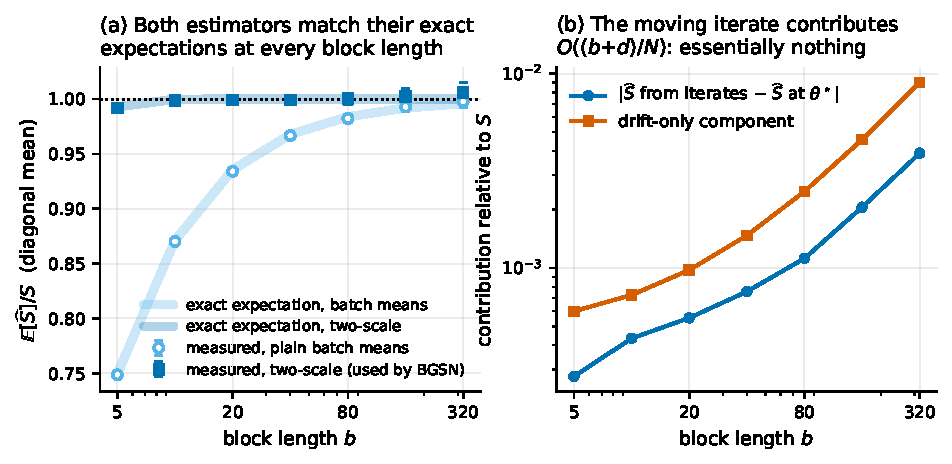
\includegraphics[width=\linewidth]{fig2_lrv.pdf}}{\fbox{\parbox{0.9\linewidth}{\centering\vspace{2em}\texttt{\detokenize{fig2_lrv}} pending\vspace{2em}}}}
\caption{\textbf{The long-run covariance estimator, and why the moving iterate does not
spoil it.} (a) Measured $\E[\widehat S]/S$ against block length: plain batch means follow
the closed-form bias $1-\Delta/(bS)$ (no fitted constants), while the two-scale form is
unbiased at every $b$, as \Cref{thm:lrv} predicts under geometric mixing.
(b) The algorithm's block gradients decomposed exactly into the score at $\ts$ and the
drift $\widehat H_t(\theta_{t-1}-\ts)$. The drift's contribution to $\widehat S$ is $0.1\%$
of $S$ at $b=20$ and $0.9\%$ at $b=320$, growing like $(b+d)/N$ as
\Cref{thm:lrv} predicts, and the estimator built from the algorithm's iterates is
indistinguishable from the one built at $\ts$. This is why our block length need only grow like $\log N$ rather than like a power of $N$ (\Cref{rem:whyfast}).}
\label{fig:lrv}
\end{figure}


%% Figure block, shared by ../paper/main.tex and ../submission/*.tex so the caption has
%% exactly one source.
\begin{figure}[tbp]
\centering
\figorbox{fig7_lrv_rate.pdf}
\caption{\textbf{The rate claim, measured, on the object an interval actually uses.}
Both axes logarithmic; error bars are $\pm1.96$ Monte Carlo standard errors; fitted slopes in
the legends. \textbf{(a)} Relative operator-norm error in estimating the whole sandwich
$\Sigma=H^{-1}SH^{-1}$. Ours is $\Hb^{-1}\Sft\Hb^{-1}$ at $b\asymp\log N$; the comparator is
overlapping batch means on the \emph{iterate} path at the block length $b_n\asymp T^{3/4}$ that
analysis requires (\Cref{app:hyper} gives the form), which uses no gradients and no curvature
estimate. Same target, so the comparison is meaningful; but read the levels, not the slopes. The
iterate-path curve is flat here, and its published $N^{-1/8}$ rate is too slow for our range to
resolve, so its fitted slope says nothing about it. What the panel shows is that over the sample
sizes we can reach, one estimator is accurate and the other is not. \textbf{(b)} Error in estimating $S$ alone, each estimator at its own optimal block
length: the two-scale form at $b\asymp\log N$ against the $-1/2$ of \Cref{thm:lrv}(iv), plain
batch means at $b\asymp N^{1/3}$ against $-1/3$.}
\label{fig:lrvrate}
\end{figure}


%% Figure block, shared by ../paper/main.tex and ../submission/*.tex so the caption has
%% exactly one source.
\begin{figure}[tbp]
\centering
\begin{minipage}[t]{0.485\linewidth}
\centering
\figorbox{fig3_gapping.pdf}
\caption{\textbf{At matched cost, a deterministic gap decorrelates curvature updates
exponentially in $m$ while random thinning only does so linearly} (\Cref{prop:gap}).
Vertical axis: $n\,\E\lVert\Hb-H\rVert_F^2$ divided by its exact independent-data value
$(\tr\Sigma)^2+\lVert\Sigma\rVert_F^2$ --- a computed constant, not a fitted normalisation.
Pale bands are the two predictions; markers are measurements with the optimisation frozen at
$\ts$, so only estimation quality is compared. $\kappa_H=(1+\phi^2)/(1-\phi^2)$ here.}
\label{fig:gap}
\end{minipage}\hfill
\begin{minipage}[t]{0.485\linewidth}
\centering
\figorbox{fig4_cost.pdf}
\caption{\textbf{The statistically correct interval is the cheaper one.} Wall-clock
milliseconds for one pass over $N=200{,}000$ observations (vertical axis, log scale) against
dimension $d$ (horizontal, log scale), single-threaded, minimum over seven interleaved
repetitions. The i.i.d.\ plug-in score covariance costs $O(d^2)$ per \emph{observation}; the
blocked long-run covariance costs $O(d^2)$ per \emph{block}. Slopes are fitted on the four
largest $d$; at this $N$ they are inflated by the one-off warm-up (see \eqref{eq:cost} and
\Cref{tab:cost}, which also gives the asymptotic exponents), and the two smallest $d$ are
dominated by fixed per-block overhead rather than by either term of \eqref{eq:cost}. The
message of the figure is the vertical separation, which holds at every $d$.}
\label{fig:cost}
\end{minipage}
\end{figure}


%% Figure block, shared by ../paper/main.tex and ../submission/*.tex so the caption has
%% exactly one source.
\begin{figure}[tbp]
\centering
\figorbox{fig5_ablations.pdf}
\caption{\textbf{Ablations.} (a) Coverage converges to nominal in $N$ for the two-scale variance,
while the dependence-blind interval converges to $0.749$, the value \Cref{prop:coverage} predicts
for this design. (b) Coverage is flat in the block length for the two-scale variance and degrades at
both ends for plain batch means --- the practical content of the $O(\rho^b)$-versus-$O(1/b)$
distinction. (c) The curvature warm-up matters, though the step-length safeguard of \eqref{eq:step}
now absorbs part of its job: with essentially no warm-up coverage on this design is $\CovNoWarmup$
against $\CovBgsnArhom$ at the default, and the relative variance on the right axis tells the same
story. On the regime-switching design, where the warm-up is load-bearing rather than merely
helpful, the effect is far larger (\Cref{tab:ablation}(c$'$)).}
\label{fig:ablation}
\end{figure}


%% Figure block, shared by ../paper/main.tex and ../submission/*.tex so the caption has
%% exactly one source.
\begin{figure}[tbp]
\centering
\figorbox{fig6_real.pdf}
\caption{\textbf{Two real hourly streams.} (a, b) Coverage of nominal $95\%$ intervals
under Protocol~A (real covariates, synthetic autoregressive errors, exact target and exact
conditional long-run covariance). The air-quality stream's median estimated variance inflation
is $\RealKappaAirq$, so dependence-blind intervals fail badly there.
(c) Coverage (left axis) against block length $b$ (horizontal, log scale) on the traffic stream,
with the free block-adequacy diagnostic
$r_j=|u_j^{\!\top}(\Sft-\Sbm)u_j|/(u_j^{\!\top}\Sbm u_j)$ --- an estimate of the relative
block-length bias of plain batch means, defined where it is first used in \Cref{sec:exp} --- on the
right axis. Three things to read. Our coverage is flat in $b$ over a fortyfold range and stays
within a few hundredths of the infeasible oracle-variance curve throughout, so the shortfall from
$0.95$ on an $\RealNMetro$-observation segment is the point estimate and not the covariance. The
dependence-blind curve sits far below at every $b$ and does not close. And $r_j$ is U-shaped, lowest
near $b=20$--$40$: it rises for small $b$, where plain batch means are biased, and again for large
$b$, where too few blocks remain to estimate anything stably --- which is what makes it a usable
guide to the block length, though not a calibration guarantee.}
\label{fig:real}
\end{figure}


%% Section body, shared verbatim by ../paper/main.tex (preprint) and
%% ../submission/body.tex (Information Sciences submission).  The designs, the eleven methods
%% compared and every secondary result are in \Cref{app:details,app:moreexp}; this section reports
%% the headline findings only, and nothing appears in both places.
Every number quoted below is generated from the saved results by the script
\file{make_tables.py} and injected as a macro, so the prose cannot drift from the data. Monte Carlo standard errors are
shown or stated everywhere.

\paragraph{Designs and methods.}
Four simulated dependent designs with $d=20$, specified in \Cref{app:dgps}: \textbf{AR-hom}
(autoregressive covariates and errors, closed-form $S$, the same inflation $\kappa=\KappaLoArhom$ in every
coordinate); \textbf{AR-het} (coordinatewise persistence, closed-form $S$, $\kappa_j$ over
$[\KappaLoArhet,\KappaHiArhet]$, so a scalar correction cannot pass); \textbf{Markov} (a Markov-modulated
Gaussian mixture with $d+1$ regimes, non-Gaussian with a discrete latent state, closed-form $S$); and
\textbf{Logistic} (a correctly specified marginal logistic model with a serially dependent latent error, so
$\ts$ is exactly the generating value while the score is autocorrelated). Covariate covariances use the
ill-conditioned design of the base paper ($\mathrm{cond}(H)$ up to $400$); \Cref{tab:wellcond} adds a
well-conditioned counterpart and \Cref{tab:real} two real hourly streams. \Cref{app:methods} lists the
eleven methods compared and their tuning; the comparisons that matter here are against the same point
estimator with plain batch means or the i.i.d.\ plug-in variance, so that only the interval changes, the
base independent-data streaming Newton method, averaged SGD and streaming AdaGrad given the \emph{true}
Hessian for their sandwich and tuned on disjoint pilot streams, and an infeasible oracle-variance interval
built from the true $H$ and $S$. \bgsn{} has no learning rate to tune.

\subsection{The failure is exactly as predicted, and it is not small}

\Cref{fig:coverage}(a) sweeps the dependence strength, comparing the coverage measured for
dependence-blind intervals against the parameter-free prediction $2\Phi(z_{0.025}/\sqrt{\kappa})-1$ of
\Cref{prop:coverage}. For $\kappa$ up to $\CovLawKappaModerate$ the largest absolute discrepancy is
$\CovLawMaxErrModerate$, of the order of the Monte Carlo standard error; \bgsn{} stays at nominal over
that range ($\CovLawMidBgsn$ at $\kappa=\CovLawMidKappa$, where the dependence-blind prediction is
$\CovLawMidPred$ and its measurement $\CovLawMidMeas\pm\CovLawMidSe$), including at $\phi=\psi=0$,
where all four intervals agree --- the control showing that the machinery is not simply widening
intervals. At the strongest dependence we tried the formula's residual gap is finite-sample, not a
failure of the formula, and the infeasible oracle interval says so: at $\kappa=\CovLawHardKappa$ it
covers only $\CovLawHardOracle$, and \bgsn{} covers $\CovLawHardBgsn$, tracking the oracle rather than
the formula. That comparison is the general point. \bgsn{}'s coverage tracks the infeasible oracle to
within Monte Carlo error at every dependence level, so whatever undercoverage remains is attributable
to the central limit theorem at finite $N$ and not to our variance estimator, whereas plain batch
means fall $1$--$3$ percentage points \emph{below} the oracle once $\kappa\ge4$ --- exactly the
$O(1/b)$ bias the two-scale correction removes.

\Cref{tab:main} gives the full picture at a common $N$. On AR-hom the base method's interval covers
$\CovSniidArhom$ and ours $\CovBgsnArhom$ against a nominal $0.95$, with the infeasible oracle at
$\CovOracleArhom$. The price is width: our interval is $\WidthRatioArhom\times$ the dependence-blind
one, which is exactly $\sqrt{\kappa}$ --- there is no free lunch, the dependence-blind interval is
simply the wrong length. AR-het is worth a separate look, because its $\kappa_j$ varies across
coordinates by construction: the dependence-blind interval's \emph{per-coordinate} coverage ranges from
$\CovPluginLoArhet$ to $\CovPluginHiArhet$ while ours ranges from $\CovBgsnLoArhet$ to
$\CovBgsnHiArhet$. No scalar inflation of the width could produce the first pattern from the second;
the whole matrix has to be estimated. Crucially, replacing \emph{only} the variance estimator repairs
the base method (row ``with our long-run variance''), and replacing only the point estimator does not:
this isolates inference as the operative component.

Three further results are reported in \Cref{app:hard,app:firstorder,app:ks}: that on the two designs
whose point estimate has not yet reached its asymptotic regime our interval tracks the one built from the
exact $H^{-1}SH^{-1}$ at the same iterate while the dependence-blind interval does not; that on a
well-conditioned design, where every point estimator is efficient and only the covariance can decide
coverage, our long-run variance is what repairs averaged SGD ($\WcCovAsgdOurs$ against
$\WcCovAsgdPlugin$); and that the Kolmogorov--Smirnov distance from our studentised error to the standard
normal is $\KsBgsnArhom$ on AR-hom against $\KsPluginArhom$ for the dependence-blind studentisation, so
the whole distribution and not merely one quantile is repaired.

\subsection{The long-run covariance estimator behaves as the theory says}

\Cref{fig:lrv}(a) plots $\E[\widehat S]/S$ against the block length together with the \emph{exact}
prediction $\sum_{|k|<b}(1-|k|/b)\Gamma_k/S$, which is closed form for this design, so the comparison
carries no approximation of its own. Plain batch means track it over the whole range ($\LrvBmAtBTwenty$
measured against $\LrvBmTheoryAtBTwenty$ predicted at $b=20$) and the two-scale estimator is within
Monte Carlo error of $1$ for $b\ge10$ ($\LrvFtAtBTwenty$ at $b=20$); the small residual at $b=5$ is the
$O(\rho^{b})$ term, only $\rho^5=0.03$ there. This is \Cref{thm:lrv}(i)--(ii) with no fitted constants.
\RefLrvRate{} measures the rate: under $b\asymp\log N$ the two-scale estimator's relative error falls
with fitted exponent $\RateExpFt$ against the $-1/2$ of \Cref{thm:lrv}(iv), while plain batch means under
their own optimal $b\asymp N^{1/3}$ schedule give $\RateExpBm$ against $-1/3$. On the whole sandwich
$\Sigma=H^{-1}SH^{-1}$, which is what an interval uses, our composite relative error falls from
$\RateOursLevelSmall$ to $\RateOursLevelBig$ while an iterate-path estimator at its own prescribed block
length sits near $\RateObmLevel$ throughout; \Cref{app:obm} is careful about what that does and does not
show.

\Cref{fig:lrv}(b) addresses the objection that a block average must span enough parameter movement to
behave like an independent draw --- the reason iterate-based batch means need $b\asymp N^{3/4}$
\citep{samsonov2025statistical}. Decomposing the block gradients exactly into the score at $\ts$ and
the drift $\widehat H_t(\theta_{t-1}-\ts)$, the drift contributes $\LrvDriftAtBTwenty$ of $S$ at $b=20$
and grows like $\tau_{b,N}=(b+d)\log^2N/N$, confirming \Cref{rem:whyfast}: because the blocks carry
gradients rather than iterates, the block length is set by the data's mixing time, not the optimiser's.

\subsection{Curvature schedules, ablations, and cost}

Three further groups of experiments are reported in \Cref{app:sched,app:abl,app:costexp}. Gapping beats
Bernoulli thinning at a matched number of rank-one updates exactly as \Cref{prop:gap} predicts, with no
measurable end-to-end effect on coverage --- which the theory also predicts, since $\Hb$ enters the limit
only through a rate --- so it is a better cost knob, not a faster one. The ablations vary $N$, the block
length, the warm-up, the ridge exponent and constant, the initial curvature scale, the curvature schedule
and the averaging variant one at a time; the results are insensitive to all of them over their admissible
ranges except the warm-up and the step-length safeguard, both of which are load-bearing on the
regime-switching design. On cost, the streaming pass grows as $d^{\StreamExpBgsn}$ for \bgsn{} and as
$d^{\StreamExpPlugin}$ once the i.i.d.\ plug-in variance is added, because the plug-in score covariance
costs $O(d^2)$ per \emph{observation} whereas our long-run covariance costs $O(d^2)$ per \emph{block};
those are exact operation counts, and in wall-clock the plug-in variant costs more at every $d$ we tried,
by a median factor of $\CostRatioPlugin$. Our valid intervals cost less than the invalid ones, not more.

\subsection{Real streams}

\Cref{tab:real} reports two protocols on hourly traffic volume on Interstate~94 and hourly PM2.5 at
twelve Beijing monitoring sites. After a fixed regression adjustment (weather plus calendar harmonics)
the residual lag-one autocorrelation is $\RealAcfMetro$ and $\RealAcfAirq$, and the median estimated
variance inflation across coordinates is $\RealKappaMetro$ for traffic and $\RealKappaAirq$ for air
quality; because $\kappa_j$ varies across coordinates, the table reports the pooled prediction
$d^{-1}\sum_j\{2\Phi(z_{0.025}/\sqrt{\kappa_j})-1\}$ next to the measurement. Protocol~A keeps the real
(strongly dependent) covariate stream and replaces the response by $x_t^{\!\top}\ts+u_t$ with $u$ an
autoregression whose coefficient equals that of the real residuals, which gives an \emph{exact} target
and an exact conditional long-run covariance while retaining real covariate dependence: \bgsn{} covers
$\RealCovBgsnMetroA$ (traffic) and $\RealCovBgsnAirqA$ (air quality) against nominal $0.95$, the
dependence-blind interval $\RealCovPluginMetroA$ and $\RealCovPluginAirqA$. Protocol~B uses the real
response and takes the full-stream $M$-estimator as the target; because that target is estimated from a
superset of each segment, the correct nominal level is $2\Phi(z_{0.025}/\sqrt{1-1/R})-1$, which we
compute exactly and report in the table header, and \bgsn{} covers $\RealCovBgsnMetroB$ and
$\RealCovBgsnAirqB$. Neither protocol alone would settle the matter --- A has an exact target but a
synthetic error process, B a real error process but an estimated target --- and they agree.

The block length is the one parameter a practitioner must think about on real data, and the free
diagnostic $r_j=|u_j^{\!\top}(\Sft-\Sbm)u_j|/(u_j^{\!\top}\Sbm u_j)$ flags when it is wrong. It is
U-shaped in $b$, rising for short blocks, where plain batch means carry the $O(1/b)$ bias, and for long
ones, where too few blocks remain for a stable estimate; over a fortyfold range in $b$ our coverage
stays flat and within a few hundredths of the infeasible oracle-variance curve (\Cref{fig:real}(c)). So
$r_j$ is a guide to choosing $b$, not a calibration guarantee, and we do not claim that it predicts
coverage (\Cref{app:realb}).


%% Figure block, shared by ../paper/main.tex and ../submission/*.tex so the caption has
%% exactly one source.
\begin{figure}[t]
\centering
\IfFileExists{fig8_hard_design.pdf}{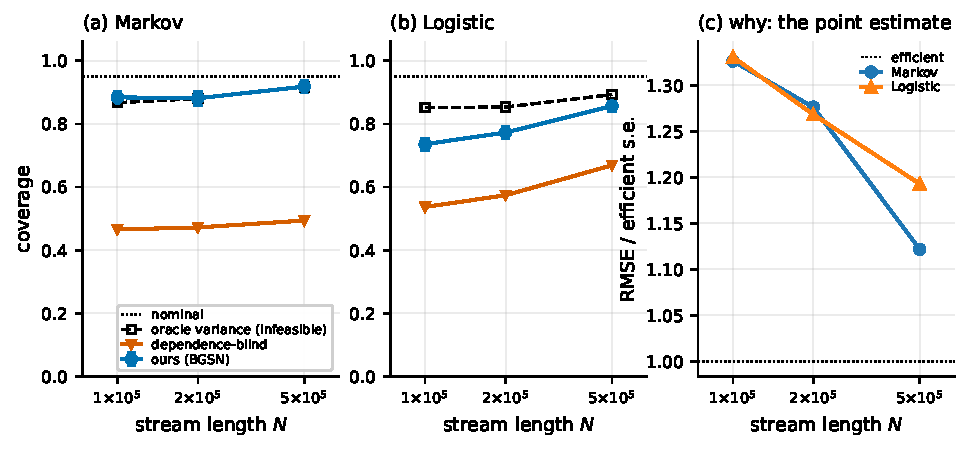
\includegraphics[width=\linewidth]{fig8_hard_design.pdf}}{\fbox{\parbox{0.9\linewidth}{\centering\vspace{2em}\texttt{\detokenize{fig8_hard_design}} pending\vspace{2em}}}}
\caption{\textbf{Separating ``the variance estimate is wrong'' from ``the central limit theorem
has not taken hold''} on the regime-switching design, whose covariate chain has an integrated
autocorrelation time of about $\HardTau$ observations. \textbf{(a)} Coverage of nominal $95\%$
intervals against $N$. The infeasible curve uses the exact $H^{-1}SH^{-1}$ at the same iterate,
so the vertical distance between it and ours is everything our covariance estimator is
responsible for; the largest such distance over the sweep is $\HardMaxGap$. Both rise towards
nominal; the dependence-blind curve does not. \textbf{(b)} The reason the left panel starts low:
the root-mean-square error of the point estimate, divided by the efficient standard error, is
still above one at small $N$, so $\sqrt N(\theta_T-\ts)$ is not yet close to its limit and no
choice of variance can give nominal coverage.}
\label{fig:hard}
\end{figure}


\IfFileExists{tab_hard.tex}{\begin{table}[tbp]
\centering
\small
\caption{\textbf{On the two designs whose point estimate has not converged, our interval tracks the infeasible oracle interval at every sample size} ($d=20$, $b=20$; $R$ decreases from 200 at the smallest $N$ to 150 at the largest, since what is being measured is the gap between the first two columns and a Monte Carlo standard error near $0.01$ is ample for it). \emph{ours} is \bgsn{}; \emph{oracle} uses the exact $H^{-1}SH^{-1}$ at the same iterate and is infeasible; \emph{blind} uses the i.i.d.\ plug-in. \emph{err} is the root-mean-square error divided by the efficient standard error, so $\mathrm{err}=1$ means the point estimate has reached the asymptotic regime, and \emph{clips} counts activations of the step-length safeguard out of $N/b$ blocks. At $N=200{,}000$ neither design is nominal because $\mathrm{err}>1$: the central limit theorem has not taken hold, which no variance estimator can repair. What our estimator is responsible for is the difference between the \emph{ours} and \emph{oracle} columns, and the largest such difference over both designs and all four sample sizes is $0.116$. The \emph{blind} column is the one that does not converge. Note that \emph{clips} does not grow with $N$, which is the empirical content of Proposition~\ref{prop:shift}.}
\label{tab:hard}
\begin{tabular}{lrccccr}
\toprule
design & $N$ & ours & oracle & blind & err & clips \\
\midrule
Markov & 100{,}000 & 0.884 & 0.867 & 0.466 & 1.33 & 8 \\
 & 200{,}000 & 0.881 & 0.880 & 0.472 & 1.28 & 8 \\
 & 500{,}000 & 0.918 & 0.917 & 0.494 & 1.12 & 7 \\
\midrule
Logistic & 100{,}000 & 0.736 & 0.852 & 0.537 & 1.33 & 2 \\
 & 200{,}000 & 0.773 & 0.853 & 0.574 & 1.27 & 2 \\
 & 500{,}000 & 0.857 & 0.893 & 0.669 & 1.19 & 2 \\
\bottomrule
\end{tabular}
\end{table}
}{}

\IfFileExists{tab_wellcond.tex}{\begin{table}[tbp]
\centering
\small
\caption{\textbf{A well-conditioned dependent design isolates the inference question} ($\Sigma_x=I$, so $\mathrm{cond}(H)=1.00$; otherwise identical to the AR-hom column of \Cref{tab:main}: $d=20$, $N=200{,}000$, $b=20$, $\kappa=2.92$, $R=300$). Here every point estimator is efficient (\emph{err} $\approx1$), so coverage is decided by the covariance estimate alone. Averaged SGD with our long-run variance is calibrated; the same estimator with the i.i.d.\ plug-in is not, by the factor $\sqrt{\kappa}=1.71$ in width that Proposition~\ref{prop:coverage} predicts. On the ill-conditioned designs of \Cref{tab:main} the first-order baselines cannot be read this way, because there their point estimates have not converged.}
\label{tab:wellcond}
\resizebox{\ifdim\width>\linewidth\linewidth\else\width\fi}{!}{%
\begin{tabular}{lccc}
\toprule
method & cov & w & err \\
\midrule
\textbf{BGSN} (this paper) & \textbf{0.942} & 1.00 & 1.03 \\
\quad with plain batch means & 0.933 & 0.97 & 1.03 \\
\quad with the i.i.d.\ plug-in variance & 0.743 & 0.59 & 1.03 \\
streaming Newton, i.i.d.\ theory & 0.740 & 0.59 & 1.03 \\
ASGD + our long-run variance & 0.931 & 1.00 & 1.07 \\
ASGD, i.i.d.\ plug-in & 0.721 & 0.59 & 1.07 \\
ASGD + random scaling & 0.917 & 1.28 & 1.07 \\
AdaGrad + our long-run variance & \textbf{0.943} & 1.00 & 1.03 \\
oracle variance \emph{(infeasible)} & \textbf{0.941} & 1.00 & 1.03 \\
\bottomrule
\end{tabular}
}
\end{table}
}{}

\IfFileExists{tab_real.tex}{\begin{table}[t]
\centering
\small
\setlength{\tabcolsep}{4pt}
\caption{\textbf{Real hourly streams.} Protocol A: real covariates, synthetic autoregressive errors whose coefficient equals the AR(1) coefficient of the real residuals, so the target and the long-run covariance are exact conditionally on the covariate path. Protocol B: fully real response, target the full-stream $M$-estimator; because that target is estimated from a superset of each segment, the correct nominal level for this comparison is $2\Phi(z_{0.025}/\sqrt{1-1/R})-1$, reported in the header. Traffic: $n=8000$ per segment, $b=40$. Air quality: $n=10000$ per segment, $b=50$, pooled over 12 monitoring sites.}
\label{tab:real}
\begin{tabular}{lcccc}
\toprule
& \multicolumn{2}{c}{traffic (I-94)} & \multicolumn{2}{c}{air quality (PM2.5)} \\
\cmidrule(lr){2-3}\cmidrule(lr){4-5}
method & A: exact truth & B: full-stream target & A: exact truth & B: full-stream target \\
\midrule
\emph{nominal} & 0.950 & 0.976 & 0.950 & 0.994 \\
\midrule
\textbf{BGSN} (this paper) & 0.818 & 0.795 & 0.893 & 0.858 \\
\quad with plain batch means & 0.814 & 0.795 & 0.892 & 0.816 \\
\quad with the i.i.d.\ plug-in variance & 0.597 & 0.682 & 0.543 & 0.361 \\
streaming Newton, i.i.d.\ theory & 0.580 & 0.682 & 0.500 & 0.365 \\
ASGD + our long-run variance & 0.564 & 0.523 & 0.331 & 0.330 \\
ASGD, i.i.d.\ plug-in & 0.391 & 0.455 & 0.198 & 0.212 \\
ASGD + random scaling & 0.571 & 0.568 & 0.422 & 0.486 \\
oracle variance \emph{(infeasible)} & 0.773 & -- & 0.788 & -- \\
\midrule
\multicolumn{5}{l}{\emph{stream diagnostics}}\\
residual AR(1) coefficient & \multicolumn{2}{c}{0.756} & \multicolumn{2}{c}{0.909 (median over sites)} \\
$R^2$ & \multicolumn{2}{c}{0.782} & \multicolumn{2}{c}{0.327} \\
block-adequacy $r_j$ & 0.163 & 0.271 & 0.186 & 0.302 \\
\bottomrule
\end{tabular}
\end{table}
}{}

\IfFileExists{tab_ablation.tex}{\begin{table}[tbp]
\centering
\small
\caption{\textbf{Ablations} on the homogeneous autoregressive design ($d=20$, $\kappa=2.92$, $R=250$). \emph{cov} columns are coverage of nominal 95\% intervals using the two-scale, plain batch-means, and i.i.d.\ plug-in variance respectively; \emph{eff} is the empirical variance of the point estimate divided by its asymptotic value ($1.00$ is efficient); \emph{adeq} is the free block-adequacy diagnostic $r_j$, an estimate of the relative block-length bias of plain batch means. The three coverage columns use the two-scale, plain batch-means and i.i.d.\ plug-in variance respectively. In panel~(i) the designs are abbreviated AR (autoregressive), AR-s (strongly autoregressive) and Mkv (regime-switching); the number of times the safeguard acted is in the text. Panel (c$'$) is on the regime-switching design and is the reason the default warm-up is $c_{\mathrm w}=200$ rather than $50$: there, $50d$ consecutive observations span only about thirty regime visits, the curvature estimate is still rank-starved, and the $1/t$ schedule diverges. The warm-up must span enough effectively distinct design points, which is not the same as enough observations. Panel (i) varies how the blocked step is safeguarded: \emph{none} is the raw $1/t$ step, \emph{cap} is the step-length safeguard of \eqref{eq:step} at $c_D=1$ (our default) with \emph{cap 0.25} and \emph{cap 4} changing $c_D$ by a factor of four either way, \emph{shift} is the rejected schedule shift of \Cref{app:t0}, and \emph{both} applies the two together; \emph{clips} counts how many of the $10{,}000$ blocks the safeguard acted on. \emph{eff} is in scientific notation where the unsafeguarded step diverges. Panel (j) is on a short stream ($N=4000$, $d=11$, the length of a real-data evaluation segment) and varies the cap on the warm-up as a fraction of the stream; $\varpi_{\mathrm w}=1$ means uncapped, which spends $2200$ of the $4000$ observations on curvature and leaves $45$ blocked steps.}
\label{tab:ablation}
\small
\setlength{\tabcolsep}{4pt}
\resizebox{\ifdim\width>\linewidth\linewidth\else\width\fi}{!}{%
\begin{tabular}{llrrrrr}
\toprule
panel & setting & eff & 2-scale & BM & plug-in & $r_j$ \\
\midrule
\multirow{5}{*}{(a) length $N$} & $N=25{,}000$ & 1.23 & 0.930 & 0.922 & 0.710 & 0.086 \\
 & $N=50{,}000$ & 1.08 & 0.937 & 0.931 & 0.731 & 0.072 \\
 & $N=100{,}000$ & 1.04 & 0.947 & 0.938 & 0.733 & 0.069 \\
 & $N=200{,}000$ & 1.04 & 0.947 & 0.937 & 0.736 & 0.069 \\
 & $N=400{,}000$ & 1.10 & 0.941 & 0.934 & 0.729 & 0.069 \\
\midrule
\multirow{8}{*}{(b) block $b$} & $b=5$ & 1.02 & 0.948 & 0.905 & 0.736 & 0.325 \\
 & $b=10$ & 1.03 & 0.949 & 0.926 & 0.737 & 0.149 \\
 & $b=20$ & 1.04 & 0.947 & 0.937 & 0.736 & 0.069 \\
 & $b=40$ & 1.04 & 0.946 & 0.943 & 0.737 & 0.041 \\
 & $b=80$ & 1.05 & 0.946 & 0.944 & 0.738 & 0.045 \\
 & $b=160$ & 1.06 & 0.946 & 0.944 & 0.734 & 0.060 \\
 & $b=320$ & 1.07 & 0.943 & 0.944 & 0.738 & 0.085 \\
 & $b=640$ & 1.10 & 0.938 & 0.942 & 0.733 & 0.118 \\
\midrule
\multirow{7}{*}{(c) warm-up} & $c_{\mathrm w}=0.5$ & 1.13 & 0.928 & 0.921 & 0.724 & 0.069 \\
 & $c_{\mathrm w}=5$ & 1.06 & 0.941 & 0.931 & 0.730 & 0.069 \\
 & $c_{\mathrm w}=25$ & 1.04 & 0.944 & 0.936 & 0.737 & 0.068 \\
 & $c_{\mathrm w}=50$ & 1.04 & 0.944 & 0.935 & 0.741 & 0.068 \\
 & $c_{\mathrm w}=100$ & 1.01 & 0.949 & 0.941 & 0.739 & 0.069 \\
 & $c_{\mathrm w}=200$ & 1.04 & 0.947 & 0.938 & 0.733 & 0.069 \\
 & $c_{\mathrm w}=500$ & 1.12 & 0.937 & 0.927 & 0.713 & 0.069 \\
\midrule
\multirow{4}{*}{(c$'$) warm-up, Mkv} & $c_{\mathrm w}=50$ & 2.19 & 0.848 & 0.812 & 0.452 & 0.239 \\
 & $c_{\mathrm w}=100$ & 1.76 & 0.879 & 0.851 & 0.467 & 0.238 \\
 & $c_{\mathrm w}=200$ & 1.41 & 0.907 & 0.877 & 0.495 & 0.237 \\
 & $c_{\mathrm w}=500$ & 1.21 & 0.923 & 0.900 & 0.536 & 0.235 \\
\midrule
\multirow{10}{*}{(d) ridge} & $c_\iota{=}0,\ \qr{=}0.2$ & 1.04 & 0.949 & 0.940 & 0.741 & 0.069 \\
 & $c_\iota{=}0.001,\ \qr{=}0.2$ & 1.04 & 0.949 & 0.940 & 0.740 & 0.069 \\
 & $c_\iota{=}0.01,\ \qr{=}0.2$ & 1.04 & 0.947 & 0.937 & 0.736 & 0.069 \\
 & $c_\iota{=}0.1,\ \qr{=}0.2$ & 1.04 & 0.931 & 0.920 & 0.703 & 0.069 \\
 & $c_\iota{=}1,\ \qr{=}0.2$ & 3.07 & 0.605 & 0.591 & 0.405 & 0.069 \\
 & $c_\iota{=}0.01,\ \qr{=}0.05$ & 1.03 & 0.943 & 0.931 & 0.729 & 0.069 \\
 & $c_\iota{=}0.01,\ \qr{=}0.1$ & 1.03 & 0.946 & 0.934 & 0.732 & 0.069 \\
 & $c_\iota{=}0.01,\ \qr{=}0.24$ & 1.04 & 0.948 & 0.938 & 0.737 & 0.069 \\
 & $c_\iota{=}0.01,\ \qr{=}0.4$ & 1.04 & 0.949 & 0.939 & 0.740 & 0.069 \\
 & $c_\iota{=}0.01,\ \qr{=}0.49$ & 1.04 & 0.949 & 0.940 & 0.740 & 0.069 \\
\midrule
\multirow{5}{*}{(e) $H_0$ scale} & $\lambda_0=1e-08$ & 1.04 & 0.947 & 0.937 & 0.736 & 0.069 \\
 & $\lambda_0=1e-06$ & 1.04 & 0.947 & 0.937 & 0.736 & 0.069 \\
 & $\lambda_0=0.0001$ & 1.04 & 0.947 & 0.937 & 0.736 & 0.069 \\
 & $\lambda_0=0.01$ & 1.04 & 0.947 & 0.937 & 0.736 & 0.069 \\
 & $\lambda_0=1$ & 1.03 & 0.947 & 0.935 & 0.734 & 0.069 \\
\midrule
\multirow{7}{*}{(f) curvature} & $m=1,\ p=1$ & 1.02 & 0.949 & 0.940 & 0.740 & 0.069 \\
 & $m=1,\ p=0.5$ & 1.02 & 0.949 & 0.940 & 0.739 & 0.069 \\
 & $m=1,\ p=0.2$ & 1.03 & 0.948 & 0.939 & 0.739 & 0.069 \\
 & $m=1,\ p=0.05$ & 1.03 & 0.948 & 0.937 & 0.737 & 0.069 \\
 & $m=1,\ p=1$ & 1.02 & 0.949 & 0.940 & 0.740 & 0.069 \\
 & $m=5,\ p=1$ & 1.03 & 0.949 & 0.938 & 0.737 & 0.069 \\
 & $m=20,\ p=1$ & 1.04 & 0.947 & 0.937 & 0.736 & 0.069 \\
\midrule
\midrule
\multirow{5}{*}{(g) strong dep.} & $b=20$ & 1.04 & 0.944 & 0.921 & 0.558 & 0.177 \\
 & $b=40$ & 1.05 & 0.946 & 0.934 & 0.556 & 0.082 \\
 & $b=80$ & 1.07 & 0.948 & 0.942 & 0.553 & 0.053 \\
 & $b=160$ & 1.09 & 0.947 & 0.946 & 0.555 & 0.063 \\
 & $b=320$ & 1.11 & 0.945 & 0.946 & 0.549 & 0.086 \\
\midrule
\multirow{3}{*}{(h) averaged} & $N=25{,}000$ & 1.28 & 0.923 & 0.916 & 0.701 & 0.079 \\
 & $N=100{,}000$ & 1.11 & 0.937 & 0.927 & 0.718 & 0.064 \\
 & $N=400{,}000$ & 1.13 & 0.939 & 0.930 & 0.725 & 0.067 \\
\midrule
\multirow{18}{*}{(i) safeguard} & AR, none & 1.05 & 0.947 & 0.937 & 0.733 & 0.069 \\
 & AR, shift & 1.07 & 0.942 & 0.935 & 0.729 & 0.069 \\
 & AR, cap & 1.04 & 0.947 & 0.937 & 0.736 & 0.069 \\
 & AR, cap 0.25 & 1.04 & 0.945 & 0.937 & 0.736 & 0.069 \\
 & AR, cap 4 & 1.04 & 0.948 & 0.937 & 0.736 & 0.069 \\
 & AR, both & 1.07 & 0.942 & 0.935 & 0.728 & 0.069 \\
 & AR-s, none & 1.22 & 0.922 & 0.897 & 0.537 & 0.177 \\
 & AR-s, shift & 1.12 & 0.936 & 0.911 & 0.527 & 0.177 \\
 & AR-s, cap & 1.04 & 0.944 & 0.921 & 0.558 & 0.177 \\
 & AR-s, cap 0.25 & 1.05 & 0.943 & 0.920 & 0.553 & 0.177 \\
 & AR-s, cap 4 & 1.05 & 0.943 & 0.918 & 0.559 & 0.177 \\
 & AR-s, both & 1.12 & 0.936 & 0.911 & 0.527 & 0.177 \\
 & Mkv, none & \ensuremath{1.1\times10^{14}} & 0.228 & 0.204 & 0.484 & 0.896 \\
 & Mkv, shift & 3.08 & 0.785 & 0.746 & 0.372 & 0.242 \\
 & Mkv, cap & 1.41 & 0.907 & 0.877 & 0.495 & 0.237 \\
 & Mkv, cap 0.25 & 1.59 & 0.883 & 0.848 & 0.480 & 0.237 \\
 & Mkv, cap 4 & \ensuremath{4.3\times10^{7}} & 0.518 & 0.484 & 0.526 & 0.520 \\
 & Mkv, both & 3.10 & 0.785 & 0.745 & 0.372 & 0.242 \\
\midrule
\multirow{5}{*}{(j) warm-up frac.} & $\varpi_{\mathrm w}=0.02$ & 1.40 & 0.937 & 0.946 & 0.723 & 0.190 \\
 & $\varpi_{\mathrm w}=0.05$ & 1.28 & 0.935 & 0.939 & 0.721 & 0.197 \\
 & $\varpi_{\mathrm w}=0.10$ & 1.28 & 0.929 & 0.930 & 0.715 & 0.203 \\
 & $\varpi_{\mathrm w}=0.25$ & 1.50 & 0.880 & 0.894 & 0.644 & 0.233 \\
 & $\varpi_{\mathrm w}=1.00$ & 2.51 & 0.787 & 0.789 & 0.515 & 0.281 \\
\bottomrule
\end{tabular}
}
\end{table}
}{}

\IfFileExists{tab_cost.tex}{\begin{table}[t]
\centering
\small
\caption{\textbf{Cost.} Wall-clock milliseconds for one pass over $N=200{,}000$ observations, single-threaded, median of 7 runs, and the empirical exponent $s$ in time $\propto d^{s}$ fitted on the four largest $d$. The i.i.d.\ plug-in score covariance that the independent-data theory prescribes costs $O(d^2)$ per \emph{observation}, so the dependence-blind interval is more expensive than our long-run interval, which costs $O(d^2)$ per \emph{block}.}
\ \emph{Asymptotic} exponents are the same exact counts evaluated at $N=10^{8}$, where the one-off $O(c_{\mathrm w}d^{3})$ warm-up is negligible and \eqref{eq:cost} reduces to $O(dN)$; at the $N$ used here the warm-up inflates the exponent, which is why the measured value exceeds one.}
\label{tab:cost}
\begin{tabular}{lrrrrrrrr}
\toprule
method & $d{=}5$ & $d{=}10$ & $d{=}20$ & $d{=}40$ & $d{=}80$ & $d{=}160$ & $s_{\mathrm{time}}$ & $s_{\mathrm{flop}}$ & $s_{\infty}$ \\
\midrule
\textbf{BGSN} (long-run interval) & 78.0 & 11.6 & 31.3 & 78.4 & 448.1 & 2697.5 & 2.18 & 1.56 & 1.00 \\
\quad with the i.i.d.\ plug-in variance & 43.4 & 79.6 & 241.6 & 632.2 & 2355.5 & 12448.9 & 1.90 & 1.91 & 1.86 \\
streaming Newton, Bernoulli $p=1/d$ & 46.3 & 21.3 & 15.1 & 169.5 & 457.7 & 2677.6 & 2.38 & 1.56 & -- \\
streaming Newton, every observation ($p=1$) & 77.0 & 292.8 & 840.9 & 2214.2 & 9754.7 & 46629.9 & 1.95 & 1.97 & 1.97 \\
ASGD (first order, random scaling) & 8.8 & 5.2 & 32.3 & 81.3 & 168.3 & 478.2 & 1.27 & -- & -- \\
offline HAC, $L=100$ \emph{(not streaming)} & 1568.3 & 2296.9 & 6894.0 & 21089.4 & -- & -- & -- & -- & -- \\
\bottomrule
\end{tabular}
\end{table}
}{}

\section{Related work}
\label{sec:related}

%% Section body, shared verbatim by ../paper/main.tex (preprint) and
%% ../submission/body.tex (Information Sciences submission).  The literatures are surveyed in full,
%% with their citations, in sec_related_detail.tex (\Cref{app:related}); this section states only
%% where our contribution begins and ends.  Nothing is duplicated between the two.
This paper sits at the intersection of four literatures. \Cref{app:related} surveys each with its
citations; here we state only the boundaries of what is new, because that is what a reader needs in
order to judge the contribution.

\paragraph{Streaming second-order methods at $O(dN)$ cost.}
Inversion-free stochastic Newton methods maintain a running inverse curvature estimate by rank-one
Sherman--Morrison updates. Our starting point is \citet{godichonbaggioni2025adaptive}, who thin those
updates with a Bernoulli variable and take mini-batches of size $d$ to reach $O(dN)$ total cost with
asymptotic efficiency. \textbf{The $O(dN)$ budget and the idea of skipping curvature updates are
theirs, not ours.} All of this work assumes independent observations. Ours adds the analysis of the
rank-one recursion when the accumulated terms are dependent, the replacement of Bernoulli thinning by
a deterministic gap (\Cref{prop:gap}), and intervals.

\paragraph{Online inference for stochastic approximation.}
Under independent sampling this is a mature area, from plug-in and batch-means variance estimators for
averaged stochastic gradient descent \citep{chen2020statistical,zhu2023online} to random scaling, which
estimates nothing at all \citep{lee2022fast}, and including the minimax rate for \emph{Hessian-free}
covariance estimation from the iterate path \citep{ni2026online}, which is close to attained
\citep{wei2026refining}. \textbf{Online estimation of the instantaneous sandwich under independent data is
therefore not new, and none of these is a claim we duplicate}: what we take is the batch-means template,
and what we add is the block-\emph{gradient} construction and its consequence for the rate
(\Cref{rem:whyfast}). The two papers that do give online covariance estimation for streaming
\emph{second-order} methods \citep{kuang2026online,wang2026inference} are under independent data, target
the instantaneous sandwich, and require the gradient noise to be a martingale difference for the
algorithm's filtration --- exactly the condition temporal dependence destroys.

\paragraph{Stochastic approximation on dependent data.}
Convergence under Markovian or mixing noise is classical, and modern rates are available for
Markov-chain gradient descent. \citet{godichonbaggioni2023learning} identify blocked or growing
mini-batches as the device that breaks dependence, with $L^2$ rates but no central limit theorem and
no inference: \textbf{blocked gradients as a dependence-breaking device are theirs.} On the inference
side, \citet{liu2023mixing} give a multiplier bootstrap for $\phi$-mixing streams,
\citet{li2023markovian} the functional central limit theorem and the semiparametric efficiency bound
$H^{-1}SH^{-1}$ under Markovian sampling, \citet{samsonov2025statistical} Berry--Esseen bounds and an
overlapping-batch-means variance for \emph{linear} stochastic approximation, and
\citet{roy2023online} an online batch-means estimator of the Markovian long-run sandwich.
\textbf{The long-run sandwich limit, the efficiency bound, and the existence of online long-run
covariance estimators under dependence are all prior art} --- for first-order methods. Every one of
these works is first-order; none maintains a curvature inverse, and the two that estimate a long-run
covariance do so from the iterate path, at $O(N^{-1/8})$, with block lengths that must grow like
$N^{3/4}$ \citep[Prop.~2, Cor.~2]{samsonov2025statistical}. \Cref{rem:whyfast} explains why block
gradients escape that constraint and \Cref{thm:lrv} quantifies the gain.

\paragraph{Long-run variance estimation.}
The statistical device is heteroskedasticity- and autocorrelation-consistent covariance estimation and the
batch-means literature it shares with simulation output analysis. The two-scale correction we use is the
flat-top lag window of \citet{politis1995bias}, recast as ``lugsail'' by \citet{vats2022lugsail}, which
\citet[Eqs.~(15) and (17)]{singh2025utility} bring to stochastic gradient descent under independent data.
\textbf{We do not claim the correction.} We claim the bias order it attains at block-gradient resolution
under geometric mixing --- the property that makes $b\asymp\log N$ admissible --- and the streaming
implementation. The population sandwich asymptotics for dependent $M$-estimation that we use are likewise
standard.


\section{Limitations}
\label{sec:limits}

We list the boundaries of the result plainly, because several of them are load-bearing.

\paragraph{Memory is $O(d^2)$, not $O(d)$.}
The $O(dN)$ claim is about \emph{time}. The method stores a $d\times d$ inverse curvature
estimate and two $d\times d$ covariance accumulators, so memory is $O(d^2)$; this is
inherited from the independent-data method we extend and is not something we improve. For
$d$ in the thousands this is the binding constraint, and a sketched or diagonal-plus-low-rank
curvature representation---as in \citet{kuang2026online,wang2026inference,godichonbaggioni2026complexity}---%
would be the natural remedy. Whether the block-gradient long-run covariance estimator
survives such a compression is open.

\paragraph{Geometric mixing is a real restriction, and the block length has to respect it.}
\Cref{thm:lrv} buys $b\asymp\log N$ from the geometric decay in
\Cref{lem:davydov}. Under algebraic mixing the flat-top bias is polynomial rather than
exponential and the admissible $b$ grows accordingly; long-memory streams are outside the
theory altogether. This is not merely formal: our air-quality stream has a residual lag-one
autocorrelation of $0.92$ and a variance-inflation factor around $20$, and there the
block length needed for calibrated intervals is an order of magnitude larger than for the
traffic stream (\Cref{tab:real}). The free diagnostic
$r_j=|u_j^{\!\top}(\Sft-\Sbm)u_j|/(u_j^{\!\top}\Sft u_j)$ detects the problem---it estimates
the relative block-length bias of plain batch means---but it does not remove it. It could be
turned into an automatic rule by maintaining covariance accumulators at several block scales
$b,2b,4b,\dots$ at once (one extra $O(d^2)$ update per block per scale, all from the same
block gradients) and reporting from the smallest scale at which $r_j$ falls below a
tolerance; we did not implement this, and we do not claim an automatic rule for $b$.

\paragraph{$\Sft$ need not be positive semidefinite.}
This is intrinsic to flat-top and lugsail estimators \citep[Remark~5]{singh2025utility}.
Marginal intervals need only positive scalars $u_j^{\!\top}\Sft u_j$, and the documented
fallback to $\Sbm$ never triggered in any of our runs, but a user who needs the full matrix
(for a joint test, say) must project it.

\paragraph{The curvature form is required.}
Everything rests on
$\nabla^2F(\theta)=\E[\alpha\,\Psi\Psi^{\!\top}]$, which holds for generalised linear
models, ridge and softmax regression, the geometric median and Gauss--Newton problems, but
not for a general objective. Without it there is no rank-one recursion and no
inversion-free update.

\paragraph{Warm-up is a real requirement, not an implementation detail.}
The $1/t$ schedule with a poor preconditioner leaves a slowly decaying component that
dominates the sampling error at realistic $N$: with a negligible warm-up, coverage of
nominal $95\%$ intervals fell to $\CovNoWarmup$ in our autoregressive design even though the
variance estimate stayed accurate (\Cref{tab:ablation}(c)). We give a scaling rule
($c_{\mathrm w}d$ curvature updates, with $c_{\mathrm w}=50$ throughout) and show
insensitivity above it, but this is a tuning constant, and the asymptotic theory is silent
about it. It also has a cost consequence we state rather than bury: the warm-up performs
$c_{\mathrm w}d$ rank-one updates at $O(d^2)$ each, so the total time is
$O(dN+c_{\mathrm w}d^3)$ and the advertised $O(dN)$ only bites once $N\gtrsim c_{\mathrm w}d^2$
(with $c_{\mathrm w}=50$ and $d=80$ that means $N\gtrsim3\times10^5$; at the $N=2\times10^5$ of
\Cref{tab:cost} the warm-up is comparable to the streaming pass).

\paragraph{Rates and what we do not prove.}
We give an almost sure rate and a central limit theorem, not a Berry--Esseen bound; the
first-order Markovian literature has the latter for linear stochastic approximation
\citep{samsonov2025statistical}, and we do not match it. We attain the semiparametric
efficiency bound of \citet{li2023markovian} rather than establishing it. Our
$\widetilde O(N^{-1/2})$ rate for $\Sft$ is not comparable to the minimax rate for
Hessian-free covariance estimation from an iterate path \citep{ni2026online}, because we use
more information (block gradients and a maintained curvature estimate); we make no claim
about optimality within our own information set.

\paragraph{Scope of the empirical evidence.}
All designs are convex $M$-estimation with $d\le160$ and $N\le4\times10^5$; there is no
deep-learning experiment and the theory would not support one. The dependence in the
simulated designs is stationary and geometrically decaying by construction. On the real
streams we do not know the truth, which is why we run two protocols; the semi-synthetic
protocol has an exact target but a synthetic (autoregressive) error process, and the fully
real protocol has a real error process but a target that is itself estimated---we correct
the nominal level for that exactly, but the correction assumes the segments are
approximately exchangeable, which non-stationarity would violate. Neither protocol alone
would be convincing; together they bracket the honest answer.

\paragraph{One thing we deliberately do not claim.}
Gapping improves the curvature estimate at matched cost (\Cref{prop:gap}, \Cref{fig:gap}),
but the curvature estimate enters the limit distribution only through a rate, so the
end-to-end effect on the point estimate and on coverage is second order and we could not
measure it reliably. The case for gapping is that it is free, deterministic, and provably
better than the randomised alternative---not that it changes the headline numbers.


\section{Conclusions}
\label{sec:conclusions}
%% Section body, shared verbatim by ../paper/main.tex (preprint) and
%% ../submission/body.tex (Information Sciences submission).  Information Sciences requires a
%% Conclusions section written to be intelligible outside the specialism; this is it.
On a dependent stream, a streaming quasi-Newton method can get the estimate right and the uncertainty
wrong. The error is not small and does not go away: the reported variance omits the autocovariances of the
score, so a nominal $95\%$ interval converges to a coverage below $95\%$ and stays there.
\Cref{prop:coverage} says exactly where --- at $2\Phi(z_{\alpha/2}/\sqrt{\kappa})-1$, computable from one
variance-inflation factor $\kappa$. At the inflation we measure on hourly air quality that is
$\RealPredAirq$, so more than half of the intervals a practitioner would report on that stream miss the
value they are meant to cover.

The remedy is a change of reading order rather than an extra estimation stage. Consume the stream in
contiguous blocks and take one preconditioned step per block. The block-averaged gradients are then, up to
a factor, the non-overlapping batch means of the score process, and batch means estimate exactly the
long-run variance the interval needs. The object the statistics requires and the object the computation
already produces are the same, so the resulting interval is \emph{cheaper} than the invalid one: an
instantaneous plug-in covariance costs $O(d^2)$ per observation, the blocked long-run covariance $O(d^2)$
per block. Gapping the rank-one curvature updates is the second change, and it is a cost knob rather than
an inference device.

Three practical consequences. Block length is the one parameter that needs thought, and needs less than
one might fear: because the blocks carry gradients rather than parameter values, their length is set by
how quickly the \emph{data} forget, not by how quickly the optimiser settles, so $b$ of order $\log N$
suffices where iterate-based methods need a power of $N$. Blocking has a price we pay and report: it makes
a step-size condition non-trivial, and without the $O(d)$ safeguard of \eqref{eq:step} our own method
diverges on a persistent regime-switching design. And honest intervals are wider --- on our designs
$\WidthRatioLo$--$\WidthRatioHi$ times the dependence-blind width, which is $\sqrt{\kappa}$ and not a
tuning choice. The narrower interval was never correct; it was the wrong length.

What we have not done bounds the claims, and \Cref{sec:limits} states each boundary precisely. The
construction itself is general: any streaming method that forms block gradients and maintains a curvature
estimate can report a long-run variance at no extra order of cost.


\bibliographystyle{plainnat}
\bibliography{refs}

\appendix
\section{Proofs}
\label{app:proofs}

Throughout, $C$ denotes a finite constant that may change from line to line,
$\delta_t=\theta_t-\ts$, $\eps_t=\gb_t(\ts)$, $P_t=\Hb_t^{-1}$, and
$\Lambda_k=\E[\eps_0\eps_k^{\!\top}]$. We take $\gamma_t=1/t$ throughout and ignore the
step-length safeguard $\Pi_t$ of \eqref{eq:step}; \Cref{prop:shift}, proved in
\Cref{app:shift}, shows that on the event where $\Pi_t$ is eventually inactive the safeguarded
iterates coincide with these from a finite time on, and \Cref{app:t0} treats the rejected
step-size-shift variant $\gamma_t=(t+t_0)^{-1}$ separately.
We write $n_t$ for the number of rank-one curvature
updates completed by the end of block $t$; with gap $m$ and no Bernoulli thinning,
$n_t=\lfloor tb/m\rfloor$, so $n_t\asymp t$.

\paragraph{Order of the argument.} The results are proved in the order of
\Cref{rem:ladder}: \Cref{lem:ridge} (from the ridge alone, no assumption on the iterates);
\Cref{thm:as} (uses \Cref{lem:ridge} only); the preliminary rate
$\norm{\delta_t}=O(t^{-1/2}\log^{c}t)$ (uses \Cref{thm:as} and consistency of $\Hb$, not its
rate); \Cref{thm:curv}; and then \Cref{thm:rate,thm:clt,thm:l2,thm:lrv}. Every remainder bound
below is uniform over $b\le C\log N$, which is the only regime in which \Cref{thm:lrv} uses
them, and the $b$-dependence is displayed wherever it is not $O(1)$.

\subsection{Preliminaries on dependence}

\begin{lemma}[Geometric decay of the score autocovariances]
\label{lem:davydov}
Under \Cref{as:mix}, $\opnorm{\Gamma_k}\le C\rho^{|k|}$ with $\rho=\cmix^{\nu/(2+\nu)}$,
and $\opnorm{\Lambda_k}\le C b^{-1}\rho^{(|k|-1)b}$ for $|k|\ge1$ while
$\opnorm{\Lambda_0}\le C/b$. Consequently $\sum_{k\in\mathbb Z}\opnorm{\Lambda_k}\le C/b$
and $S=\sum_k\Gamma_k$ converges absolutely.
\end{lemma}

\begin{proof}
Davydov's inequality \citep{davydov1968convergence}, in the form of
\citet[Cor.~1.1]{rio1993covariance}, gives for random variables $U\in\sigma(\xi_i,i\le0)$,
$V\in\sigma(\xi_i,i\ge k)$ with $2+\nu$ moments,
$|\Cov(U,V)|\le 8\,\alpha_{\mathrm{mix}}(k)^{\nu/(2+\nu)}\norm{U}_{2+\nu}\norm{V}_{2+\nu}$.
Applying it coordinatewise to $g_0$ and $g_k$ and using \Cref{as:mix} gives the first
claim. For the second, $\Lambda_k=b^{-2}\sum_{i\in B_0}\sum_{j\in B_k}\Gamma_{j-i}$; for
$k\ge1$ every lag $j-i$ is at least $(k-1)b+1$, so
$\opnorm{\Lambda_k}\le b^{-2}\cdot b^2\cdot C\rho^{(k-1)b}$, and for $k=0$,
$\opnorm{\Lambda_0}\le b^{-2}\sum_{|l|<b}(b-|l|)C\rho^{|l|}\le Cb^{-1}$.
Summing the geometric series gives $\sum_k\opnorm{\Lambda_k}\le C/b$.
\end{proof}

\begin{lemma}[Martingale--coboundary decomposition]
\label{lem:gordin}
Let $(\zeta_t)_{t\ge1}$ be stationary, centred, $\R^{q}$-valued, $\Fil_t$-measurable with
$\Fil_t=\sigma(\xi_i:i\le tb)$, and let $\E\norm{\zeta_1}^{2+\nu}<\infty$ under
\Cref{as:mix}. Then $\sum_{n\ge0}\norm{\E[\zeta_{n}\mid\Fil_0]}_{2}<\infty$, the series
$z_t=\sum_{n\ge0}\E[\zeta_{t+n}\mid\Fil_t]$ converges in $L^2$, and
\begin{equation}
\zeta_t \;=\; m_{t+1}+z_t-z_{t+1},
\qquad m_{t+1}=z_{t+1}-\E[z_{t+1}\mid\Fil_t],
\label{eq:gordin}
\end{equation}
where $(m_t)$ is a stationary martingale difference sequence with respect to $(\Fil_t)$ and
$\E\norm{m_1}^2<\infty$, $\E\norm{z_1}^2<\infty$. Moreover
$\E[m_1m_1^{\!\top}]=b^{-1}S$ when $\zeta_t=\eps_t$.
\end{lemma}

\begin{proof}
For $U$ that is $\sigma(\xi_i:i\ge n)$-measurable with $2+\nu$ moments, the standard
consequence of strong mixing (see \citealt[Ch.~1]{rio2017asymptotic}) is
$\norm{\E[U\mid\Fil_0]}_2\le C\,\alpha_{\mathrm{mix}}(n)^{\nu/(2(2+\nu))}\norm{U}_{2+\nu}$,
which under \Cref{as:mix} decays geometrically in $n$ and is therefore summable; this is
Gordin's condition, and \eqref{eq:gordin} together with the stated moment bounds is Gordin's
decomposition; see \citet[Ch.~5]{hall1980martingale}. Summing \eqref{eq:gordin} telescopes
the coboundary, so $\sum_{t\le T}\zeta_t=\sum_{t\le T}m_{t+1}+z_1-z_{T+1}$; dividing by
$\sqrt T$ and using $z_{T+1}/\sqrt T\to0$ in probability identifies
$\lim T^{-1}\Var(\sum_{t\le T}\zeta_t)=\E[m_1m_1^{\!\top}]$, which for $\zeta_t=\eps_t$ is
$b^{-1}S$ by \eqref{eq:S}.
\end{proof}

\begin{lemma}[Weighted sums with adapted weights: convergence and rate]
\label{lem:series}
Let $(\zeta_t)$ be as in \Cref{lem:gordin}, let $(A_t)$ be $\Fil_{t-1}$-measurable random
matrices, and let $(\gamma_t)$ be deterministic and non-increasing. Suppose there are
deterministic $(c_t)$, $(u_t)$ and a finite random $\Lambda$ with, almost surely for all $t$,
\begin{equation}
\opnorm{A_t}\le\Lambda c_t
\qquad\text{and}\qquad
\opnorm{\gamma_{t+1}A_{t+1}-\gamma_tA_t}\le\Lambda u_t ,
\label{eq:weightcond}
\end{equation}
and write $V_T=\sum_{t\le T}\gamma_t^2c_t^2$ and $U_T=\sum_{t\le T}u_t$. Then for every
$\varpi>0$, almost surely,
\begin{equation}
\Big\lVert\sum_{t\le T}\gamma_tA_t\zeta_t\Big\rVert
=O\big(V_T^{1/2}\log^{1/2+\varpi}T\big)
+O\big(U_T\log^{1+\varpi}T\big)
+O\big(\gamma_Tc_T\,T^{1/2+\varpi}\big).
\label{eq:lemrate}
\end{equation}
If moreover $V_\infty<\infty$, $U_\infty<\infty$ and $\gamma_Tc_TT^{1/2+\varpi}\to0$ for some
$\varpi>0$, then $\sum_t\gamma_tA_t\zeta_t$ converges almost surely.
\end{lemma}

\begin{proof}
\emph{Localisation.} For $K\in\mathbb N$ replace $A_t$ by
\[
A_t\,\ind\Big\{\sup_{s\le t}\max\big(\opnorm{A_s}/c_s,\;
\opnorm{\gamma_{s+1}A_{s+1}-\gamma_sA_s}/u_s\big)\le K\Big\},
\]
which is still $\Fil_{t-1}$-measurable (the indicator is decreasing in $t$ and $\Fil_{t-1}$-measurable at
each $t$ because it involves $A_s$ only for $s\le t$, and $A_{s+1}$ enters only through
$s+1\le t$). On $\{\Lambda\le K\}$ the two processes agree and
$\Prob(\bigcup_K\{\Lambda\le K\})=1$, so it suffices to prove the claims under the
\emph{deterministic} envelopes $\opnorm{A_t}\le Kc_t$,
$\opnorm{\gamma_{t+1}A_{t+1}-\gamma_tA_t}\le Ku_t$. Fix $K$ and drop it.

\emph{Martingale part.} Insert \eqref{eq:gordin}: $M_T=\sum_{t\le T}\gamma_tA_tm_{t+1}$ is a
martingale, because $A_t$ is $\Fil_t$-measurable and $\E[m_{t+1}\mid\Fil_t]=0$ --- this is
the exact cancellation the decomposition buys, and it holds whatever $A_t$ does. Its
predictable quadratic variation obeys
\[
\langle M\rangle_T=\sum_{t\le T}\gamma_t^2\,\E\!\left[\norm{A_tm_{t+1}}^2\;\middle|\;\Fil_t\right]
\le K^2\sum_{t\le T}\gamma_t^2c_t^2\,v_t,
\qquad v_t:=\E\!\left[\norm{m_{t+1}}^2\mid\Fil_t\right],
\]
with $(v_t)$ stationary, non-negative and $\E v_t=\E\norm{m_1}^2<\infty$. By Tonelli
$\E\big[\sum_{t\le T}\gamma_t^2c_t^2v_t\big]=\E\norm{m_1}^2V_T$, so Markov's inequality along
$T=2^j$ and Borel--Cantelli give $\langle M\rangle_T=O(V_T\log^{\varpi}T)$ a.s.\ (and
$\langle M\rangle_\infty<\infty$ a.s.\ if $V_\infty<\infty$). The martingale law of the
iterated logarithm then gives $\norm{M_T}=O(V_T^{1/2}\log^{1/2+\varpi}T)$ a.s., and if
$\langle M\rangle_\infty<\infty$ a locally square-integrable martingale converges a.s.

\emph{Coboundary part.} Abel summation gives
\[
\sum_{t\le T}\gamma_tA_t(z_t-z_{t+1})
=\gamma_1A_1z_1-\gamma_TA_Tz_{T+1}
+\sum_{t<T}\big(\gamma_{t+1}A_{t+1}-\gamma_tA_t\big)z_{t+1}.
\]
The last sum is at most $K\sum_{t<T}u_t\norm{z_{t+1}}$, a non-negative sum with expectation
$K\E\norm{z_1}U_T$, hence $O(U_T\log^{1+\varpi}T)$ a.s.\ by Markov and Borel--Cantelli along
dyadic blocks; if $U_\infty<\infty$ its expectation is finite and it converges a.s. Finally
$\norm{\gamma_TA_Tz_{T+1}}\le K\gamma_Tc_T\norm{z_{T+1}}=O(\gamma_Tc_TT^{1/2+\varpi})$ a.s.,
because $\E\norm{z_1}^2<\infty$ and Borel--Cantelli give
$\norm{z_T}=o(T^{1/2+\varpi})$.
\end{proof}

\begin{remark}[Why the lemma is stated this way]
Three features are load-bearing and each corresponds to a place where a naive argument fails.
(i) The weights are \emph{random and adapted}: they contain $\Hb_{t-1}^{-1}$, so a lemma for
deterministic weights would not apply. Note that adaptedness is essential and not cosmetic:
for bounded adapted weights and a mixing, centred, stationary $\zeta$ the sum
$\sum_ta_t\zeta_t$ can grow like $T$ if $a_t$ is allowed to correlate with $\zeta_t$ --- take
$\zeta_t=u_t+u_{t-1}$ with $u_t$ i.i.d.\ signs and $a_t=\zeta_{t-1}$ --- which is exactly the
non-martingale obstruction. The decomposition \eqref{eq:gordin} removes it because
$\E[m_{t+1}\mid\Fil_t]=0$ \emph{exactly}, whatever $A_t$ does.
(ii) The envelope is deterministic only up to a finite random factor, which is all that is
available for weights built from the iterates; the localisation handles it.
(iii) We use a martingale law of the iterated logarithm rather than a Bernstein inequality for
mixing sums. The Bernstein inequality of \citet{merlevede2011bernstein} is stated for
uniformly \emph{bounded} summands, which \Cref{as:mix} does not provide; after
\eqref{eq:gordin} the summands form a martingale difference sequence and no such inequality
is needed. (iv) The three terms of \eqref{eq:lemrate} are needed separately: the applications
below use $\gamma_t\equiv1$, for which $U_T$ can diverge logarithmically, so a hypothesis
$U_\infty<\infty$ would be too strong.
\end{remark}

\Cref{lem:gordin,lem:series} are the technical substitute for the martingale argument used
in the independent-data analysis. Two features matter. First, the weights may be
\emph{random and adapted}, which is what we need because they involve $\Hb_{t-1}^{-1}$.
Second, the conditions \eqref{eq:weightcond} are of the form already familiar from the
independent-data theory. The vanishing ridge supplies the deterministic envelope: it forces
$\lambda_{\min}(A_{n})\ge c\,n^{1-q_{\mathrm r}}$, hence
$\opnorm{\Hb_t^{-1}}=W_{n_t}\opnorm{A_{n_t}^{-1}}\le c^{-1}n_t^{q_{\mathrm r}}=:c_t$ with
$q_{\mathrm r}<1/2$, so with $\gamma_t=1/t$ the first half of \eqref{eq:weightcond} is
$\sum_tO(t^{2q_{\mathrm r}-2})<\infty$. The second half holds because a single rank-one Riccati
update changes the preconditioner by only $O(1/t)$:

\begin{lemma}[Increments of the preconditioner]
\label{lem:incr}
\emph{(a) From the ridge alone.} Under \Cref{as:curv} and the ridge of \eqref{eq:curv} --- so
using only \Cref{lem:ridge}, with no assumption on the iterates ---
$\opnorm{\Hb_t^{-1}-\Hb_{t-1}^{-1}}=O(t^{2\qr-1})$ a.s.; hence with $\gamma_t=1/t$ and
$A_t=\Hb_{t-1}^{-1}$, $\opnorm{\gamma_{t+1}A_{t+1}-\gamma_tA_t}=O(t^{2\qr-2})$ a.s., which is
summable for $\qr<1/2$, so the second half of \eqref{eq:weightcond} holds with
$U_\infty<\infty$.

\emph{(b) Sharper, once the curvature has converged.} Under the assumptions of
\Cref{thm:curv}, $\opnorm{\Hb_t^{-1}-\Hb_{t-1}^{-1}}=O(1/t)$ a.s., so with $\gamma_t\equiv1$
and $A_t=\Hb_{t-1}^{-1}$ the increments are $u_t=O(1/t)$ and $U_T=O(\log T)$.
\end{lemma}

\begin{proof}
$\Hb_t^{-1}=W_{n_t}A_{n_t}^{-1}$, and from block $t-1$ to block $t$ the weight $W$ increases by
$O(1)$ while $A^{-1}$ changes by $O(1)$ rank-one Sherman--Morrison steps
$A^{-1}\mapsto A^{-1}-cA^{-1}uu^{\!\top}A^{-1}/(1+cu^{\!\top}A^{-1}u)$. Writing $v=A^{-1}u$, the
operator norm of one such step is $c\norm{v}^2/(1+cu^{\!\top}v)$, and since
$u^{\!\top}v=v^{\!\top}Av\ge\lambda_{\min}(A)\norm{v}^2$ we get the two bounds
\begin{equation}
\opnorm{\Delta A^{-1}}\ \le\ \min\Big\{\frac{1}{\lambda_{\min}(A)},\
\frac{c\norm{u}^2}{\lambda_{\min}(A)^2}\Big\} .
\label{eq:smbound}
\end{equation}
For (a), \Cref{lem:ridge} gives $\lambda_{\min}(A_{n})\ge c'n^{1-\qr}$, so the second bound in
\eqref{eq:smbound} is $O(n^{2\qr-2})$; multiplying by $W_{n_t}=O(t)$ and using $n_t\asymp t$
gives $\opnorm{\Hb_t^{-1}-\Hb_{t-1}^{-1}}=O(t^{2\qr-1})$, and the change in $W$ contributes
$O(1)\cdot\opnorm{A^{-1}}=O(t^{\qr-1})$, which is smaller. The stated bound on
$\gamma_{t+1}A_{t+1}-\gamma_tA_t$ then follows from $\gamma_t=1/t$ together with
$\gamma_{t+1}-\gamma_t=O(t^{-2})$ and $\opnorm{A_t}=O(t^{\qr})$.
For (b), \Cref{thm:curv} gives $A_{n_t}/n_t\to H\succ0$, so $\lambda_{\min}(A_{n_t})\ge c't$
a.s.\ for large $t$, the second bound in \eqref{eq:smbound} is $O(t^{-2})$, and multiplying by
$W_{n_t}=O(t)$ gives $O(1/t)$.
\end{proof}

\subsection{The ridge bound (\texorpdfstring{\Cref{lem:ridge}}{Lemma})}

Each curvature update adds $\iota_n e_{k_n}e_{k_n}^{\!\top}\succeq0$ along a cycling basis
direction, and the data term $\alpha_{i_n}\Psi_{i_n}\Psi_{i_n}^{\!\top}$ is positive
semidefinite, so it can only help. After $n$ updates every basis direction has received at least
$\lfloor n/d\rfloor$ ridge increments, and dropping the data terms,
\begin{equation}
A_n\ \succeq\ \lambda_0 I+\Big(\tfrac1d\textstyle\sum_{k\le n}\iota_k\Big)I .
\label{eq:ridgelb}
\end{equation}
Now the point of freezing the ridge scale. Because $\iota_k=c_\iota\varsigma_\star k^{-\qr}$ with
$\varsigma_\star$ a \emph{constant} --- measurable with respect to the first curvature-bearing
block and, by \Cref{as:curv}, almost surely finite and strictly positive whenever that block's
curvature is not identically zero --- we may sum:
\[
\sum_{k\le n}\iota_k=c_\iota\varsigma_\star\sum_{k\le n}k^{-\qr}
\ \ge\ \frac{c_\iota\varsigma_\star}{1-\qr}\,\big(n^{1-\qr}-1\big),
\]
using $\sum_{k\le n}k^{-\qr}\ge\int_1^{n+1}x^{-\qr}dx$ and $\qr<1$. Hence
$\lambda_{\min}(A_n)\ge c'n^{1-\qr}$ for all $n\ge2$ with
$c'=c_\iota\varsigma_\star/\{2d(1-\qr)\}$, and since $W_{n_t}=1+n_t$,
\[
\opnorm{\Hb_t^{-1}}=W_{n_t}\opnorm{A_{n_t}^{-1}}\le\frac{1+n_t}{c'n_t^{1-\qr}}=O(n_t^{\qr}),
\qquad
\lambda_{\min}(\Hb_t)\ge\frac{c'n_t^{1-\qr}}{1+n_t}\ \ge\ c_1n_t^{-\qr}
\]
with $c_1=c'/2$ for $n_t\ge1$. Nothing about the iterates is used, and no lower bound on the
accumulated data terms is needed --- which is exactly why the lemma may sit at the bottom of the
ladder in \Cref{rem:ladder}.

\begin{remark}[Why the scale must be frozen]
\label{rem:freeze}
Had we scaled the ridge by the \emph{running} harmonic mean $d/\tr(\Hb_k^{-1})$ --- the natural
choice, since it is available for free from the maintained inverse --- this proof would fail, and
not for a technical reason. That scale is bounded above by $d\lambda_{\min}(\Hb_k)$, so a path
along which the accumulated data terms contribute negligibly in some direction would have its
ridge shrink in step with the very eigenvalue the ridge is supposed to hold up. Concretely, the
only unconditional bound then available is $\varsigma_k\ge\lambda_0/W_k=\Theta(1/k)$, giving
$\sum_{k\le n}\iota_k=O(1)$ instead of $\Omega(n^{1-\qr})$, and a Gronwall argument in the
opposite direction shows this is tight: $\lambda_{\min}(A_n)$ can stay $O(1)$, i.e.\
$\opnorm{\Hb_n^{-1}}=\Omega(n)$, which would break the square-summability
$\sum_t\gamma_t^2\opnorm{P_{t-1}}^2<\infty$ that \Cref{thm:as} needs. The bound does hold once
$\Hb_t\to H\succ0$, but that is \Cref{thm:curv}, three rungs higher, so the argument would be
circular. Freezing the scale removes the problem at no cost: $\varsigma_\star$ serves only to
make $c_\iota$ dimensionless, and \Cref{tab:ablation}(d) shows the results are unchanged if the
scale is dropped altogether.
\end{remark}

\subsection{Consistency (\texorpdfstring{\Cref{thm:as}}{Theorem})}

Substituting $\gb_t(\theta_{t-1})=\nabla F(\theta_{t-1})+\zeta_t$ into \eqref{eq:step},
where $\zeta_t=\gb_t(\theta_{t-1})-\nabla F(\theta_{t-1})$, and expanding
$F(\theta_t)-F(\ts)$ to second order using \Cref{as:reg},
\begin{align}
F(\theta_t)-F(\ts)&\le F(\theta_{t-1})-F(\ts)
-\gamma_t\nabla F(\theta_{t-1})^{\!\top}P_{t-1}\nabla F(\theta_{t-1})\nonumber\\
&\quad-\gamma_t\nabla F(\theta_{t-1})^{\!\top}P_{t-1}\zeta_t
+\tfrac{L}{2}\gamma_t^2\opnorm{P_{t-1}}^2\norm{\gb_t(\theta_{t-1})}^2 .
\label{eq:desc}
\end{align}
The last term is summable: $\gamma_t^2\opnorm{P_{t-1}}^2=O(t^{2q_{\mathrm r}-2})$ by
\Cref{lem:ridge} with $q_{\mathrm r}<1/2$, and $\E\norm{\gb_t(\theta_{t-1})}^2\le
C+C'(F(\theta_{t-1})-F(\ts))$ by \Cref{as:mom} and Jensen. The cross term is the one that
would be handled by a martingale argument under independence. Instead, decompose
$\zeta_t=\eps_t+r_t$ with $r_t=\gb_t(\theta_{t-1})-\nabla F(\theta_{t-1})-\eps_t$, so that
\begin{equation}
\norm{r_t}\le\opnorm{\Hh_t-H}\norm{\delta_{t-1}}+L_\delta\norm{\delta_{t-1}}^2
\label{eq:rt}
\end{equation}
where $\widehat H_t$ is the block curvature; $r_t$ is dominated by
$\norm{\delta_{t-1}}$ times an $L^2$-bounded factor, and its contribution to
\eqref{eq:desc} is absorbed by the Robbins--Siegmund argument
\citep{robbins1971convergence}. The remaining term
$-\sum_t\gamma_t\nabla F(\theta_{t-1})^{\!\top}P_{t-1}\eps_t$ is handled by
\Cref{lem:series} with $A_t=\nabla F(\theta_{t-1})^{\!\top}P_{t-1}$, which is
$\Fil_{t-1}$-measurable as required. Its first condition holds because
$\opnorm{P_{t-1}}=O(t^{q_{\mathrm r}})$ with $q_{\mathrm r}<1/2$ (\Cref{lem:ridge}) and
$\E\norm{\nabla F(\theta_{t-1})}^2$ is bounded on the events
$\{\sup_{s\le t}\norm{\theta_s}\le K\}$, over which we localise and then let $K\to\infty$;
its second condition holds by \Cref{lem:incr}(a) --- which, being a consequence of
\Cref{lem:ridge} alone, keeps this rung free of \Cref{thm:curv} --- together with
$\opnorm{\nabla F(\theta_t)-\nabla F(\theta_{t-1})}\le L\norm{\theta_t-\theta_{t-1}}
=O(\gamma_t t^{q_{\mathrm r}})$. Robbins--Siegmund then gives $F(\theta_t)\to F(\ts)$ a.s.\ and
$\sum_t\gamma_t\nabla F(\theta_{t-1})^{\!\top}P_{t-1}\nabla F(\theta_{t-1})<\infty$ a.s.;
and since $\gamma_t\lambda_{\min}(P_{t-1})\ge \gamma_t/\opnorm{\Hb_{t-1}}\ge c\,t^{-1}$
(because $\opnorm{\Hb_t}$ is bounded above a.s., $\Hb_t$ being an average of terms with
$\eta'>2$ moments) we have $\sum_t\gamma_t\lambda_{\min}(P_{t-1})=\infty$; \Cref{as:ident}
then forces $\theta_t\to\ts$ a.s. \hfill$\square$

\subsection{The preliminary rate (rung (iii) of \texorpdfstring{\Cref{rem:ladder}}{the ladder})}
\label{app:prelim}

This rung is what \Cref{thm:curv} needs and \Cref{thm:as} does not give: a rate, not just
convergence. We prove it using only \Cref{lem:ridge} and \Cref{thm:as}.

\begin{lemma}[Preliminary rate]
\label{lem:prelim}
Under \Cref{as:reg,as:mom,as:curv,as:ident,as:mix}, with $\qr\in(0,1/4)$,
$\norm{\theta_T-\ts}=O(T^{-1/2}\log^{1+\varpi}T)$ almost surely, for every $\varpi>0$.
\end{lemma}

\begin{proof}
Abel summation of \eqref{eq:step} exactly as in \eqref{eq:abel} --- an algebraic identity that
uses only $\gamma_t=1/t$ --- gives \eqref{eq:decomp}:
$\delta_T=-T^{-1}H^{-1}\sum_{t\le T}\eps_t+(\mathrm A)+(\mathrm B)-(\mathrm C)$. We bound the
three remainders using only what rungs (i) and (ii) provide, namely
$\opnorm{P_{t-1}}=O(t^{\qr})$ a.s.\ (\Cref{lem:ridge}), $\theta_t\to\ts$ a.s.\
(\Cref{thm:as}), and hence, by the local Lipschitz property in \Cref{as:curv} and the
continuity in \Cref{as:mom}, $\opnorm{P_{t-1}-H^{-1}}=o(1)$ and
$\opnorm{I-P_{t-1}H}=o(1)$ a.s. Write $\rho_t=\opnorm{I-P_{t-1}H}$, so $\rho_t\to0$ a.s.

\emph{Leading term.} $T^{-1}\sum_{t\le T}\eps_t=O(T^{-1/2}\log^{1/2+\varpi}T)$ a.s.\ by the
martingale law of the iterated logarithm applied to \eqref{eq:gordin} (the coboundary
telescopes to $O(T^{-1})$ after division by $T$, using $\E\norm{z_1}^2<\infty$ and
Borel--Cantelli along $\norm{z_t}=o(t^{1/2})$ a.s.).

\emph{Term (A).} Apply \eqref{eq:lemrate} with $\gamma_t\equiv1$ and
$A_t=H^{-1}-P_{t-1}$: the envelope may be taken $c_t\equiv1$ (a finite random constant, since
$\opnorm{P_{t-1}}=O(t^{\qr})$ makes $\sup_t\opnorm{A_t}/c_t$ finite only after we note
$A_t\to0$; formally take $c_t=1$ and $\Lambda=\sup_t\opnorm{A_t}<\infty$ a.s., which holds
because $A_t\to0$ and each $A_t$ is finite). By \Cref{lem:incr}(a) the increments are
$u_t=O(t^{2\qr-1})$, so $V_T=O(T)$ and $U_T=O(T^{2\qr})$, and \eqref{eq:lemrate} gives
$\lVert\sum_{t\le T}A_t\eps_t\rVert
=O(T^{1/2}\log^{1/2+\varpi}T)+O(T^{2\qr}\log^{1+\varpi}T)+O(T^{1/2+\varpi})$.
Dividing by $T$ and using $\qr<1/4$, which is exactly where that restriction is needed,
$(\mathrm A)=O(T^{-1/2}\log^{1/2+\varpi}T)+O(T^{2\qr-1}\log^{1+\varpi}T)
=O(T^{-1/2}\log^{1/2+\varpi}T)$ a.s.

\emph{Terms (B) and (C): the bootstrap.} $(\mathrm B)=T^{-1}\sum_{t\le T}(I-P_{t-1}H)\delta_{t-1}$
so $\norm{(\mathrm B)}\le\big(\sup_{t\le T}\rho_t\big)\,\bar\delta_T$ with
$\bar\delta_T=T^{-1}\sum_{t\le T}\norm{\delta_{t-1}}$, and by \eqref{eq:rt}
$\norm{(\mathrm C)}\le CT^{-1}\sum_{t\le T}\opnorm{P_{t-1}}
(\opnorm{\Hh_t-H}\norm{\delta_{t-1}}+\norm{\delta_{t-1}}^2)$, which is
$o(1)\,\bar\delta_T$ a.s.\ because $\opnorm{P_{t-1}}\opnorm{\Hh_t-H}$ and
$\opnorm{P_{t-1}}\norm{\delta_{t-1}}$ are both $o(1)$ a.s.\ ($\delta_t\to0$ by \Cref{thm:as},
and $\opnorm{P_{t-1}}\opnorm{\Hh_t-H}\to0$ because $\opnorm{P_{t-1}}\to\opnorm{H^{-1}}$ and
$\Hh_t\to H$ in the Cesàro sense along the block index). Hence there is a random
$T_1<\infty$ and a sequence $\epsilon_T\downarrow0$ with
\begin{equation}
D_T:=\max_{t\le T}\norm{\delta_t}\ \le\ \epsilon_T D_T + R_T,
\qquad R_T=O(T^{-1/2}\log^{1/2+\varpi}T)\ \text{a.s.},
\label{eq:boot}
\end{equation}
for $T\ge T_1$, where we used $\bar\delta_T\le D_T$ and that the same bound applies to every
$t\le T$ (the right-hand side is non-decreasing in $T$). For $T$ large enough that
$\epsilon_T\le1/2$, \eqref{eq:boot} rearranges to $D_T\le2R_T$, which is the claim with
$\log^{1+\varpi}$ absorbing $\log^{1/2+\varpi}$.
\end{proof}

\noindent
Two things are worth flagging about this rung. It is the only place the restriction
$\qr<1/4$ (rather than $\qr<1/2$) is used, and it is used because at this rung the sharper
increment bound \Cref{lem:incr}(b) is not yet available. And the bootstrap in \eqref{eq:boot} is
why the rate carries a $\log$ factor rather than being clean $T^{-1/2}$; \Cref{thm:rate}
recovers the sharper statement once \Cref{thm:curv} is in hand.

\subsection{The curvature rate (\texorpdfstring{\Cref{thm:curv}}{Theorem})}

Write $Y_n=\alpha(\ts;\xi_{i_n})\Psi(\ts;\xi_{i_n})\Psi(\ts;\xi_{i_n})^{\!\top}$ and
$\tilde Y_n=\alpha(\theta_{t(n)-1};\xi_{i_n})\Psi\Psi^{\!\top}$ for the term actually
accumulated, where $t(n)$ is the block containing $i_n$. Then, by \eqref{eq:curv} and
\eqref{eq:Hbar},
\begin{multline}
\Hb_t-H
=\underbrace{\frac{\lambda_0 I}{W_{n_t}}}_{(\mathrm i)}
+\underbrace{\frac{1}{W_{n_t}}\sum_{n\le n_t}\iota_n e_{k_n}e_{k_n}^{\!\top}}_{(\mathrm{ii})}\\
+\underbrace{\frac{1}{W_{n_t}}\sum_{n\le n_t}(Y_n-H)}_{(\mathrm{iii})}
+\underbrace{\frac{1}{W_{n_t}}\sum_{n\le n_t}(\tilde Y_n-Y_n)}_{(\mathrm{iv})}.
\label{eq:Hdecomp}
\end{multline}
Since $W_{n_t}=1+n_t\asymp t$, term (i) is $O(1/t)$. For (ii),
$\opnorm{\cdot}\le n_t^{-1}\sum_{n\le n_t}\iota_n\le C n_t^{-q_{\mathrm r}}$ because
$\iota_n\le C n^{-q_{\mathrm r}}$ and $q_{\mathrm r}<1$; the same bound from below along each basis
direction gives, together with $H\succ0$,
$\lambda_{\min}(\Hb_t)\ge c\,n_t^{-q_{\mathrm r}}$ for all $t$ (this is the only place the ridge
is used, and it is what bounds $\opnorm{\Hb_t^{-1}}$ for \emph{every} $t$ rather than
eventually). Term (iv) is bounded, by the local Lipschitz property in \Cref{as:curv} and
Cauchy--Schwarz, by
$Cn_t^{-1}\sum_{n\le n_t}\norm{\theta_{t(n)-1}-\ts}\cdot\opnorm{\Psi\Psi^{\!\top}}$, which by
\Cref{lem:prelim} is
\[
O\Big(n_t^{-1}\sum_{n\le n_t}n^{-1/2}\log^{1+\varpi}n\Big)=O(n_t^{-1/2}\log^{1+\varpi}n_t)
\quad\text{a.s.}
\]

The new content is term (iii). The array $(Y_n)_{n\ge1}$ is the subsequence of a stationary
geometrically mixing sequence at spacing $m$, hence itself stationary with mixing
coefficients $\alpha_{\mathrm{mix}}(jm)\le K\cmix^{jm}$, and has $\eta'>2$ moments by
\Cref{as:curv}. Applying \Cref{lem:series} with $a_n\equiv1$ (i.e.\ its maximal-inequality
half, which does not need square-summability) gives
$\opnorm{\sum_{n\le n_t}(Y_n-H)}=O(n_t^{1/2}\log^{1/2+\varpi}n_t)$ a.s., so
$(\mathrm{iii})=O(t^{-1/2}\log^{1/2+\varpi}t)$ a.s.
Collecting the four terms, $\opnorm{\Hb_t-H}=O(t^{-\min\{q_{\mathrm r},1/2\}}\log^{c'}t)$ a.s.,
which is $O(t^{-\nu_H})$ for every $\nu_H<\min\{q_{\mathrm r},1/2\}$. Finally, on the event
$\opnorm{\Hb_t-H}\le\lambda_{\min}(H)/2$ (which holds for all large $t$ a.s.),
$\opnorm{\Hb_t^{-1}-H^{-1}}\le\opnorm{\Hb_t^{-1}}\opnorm{\Hb_t-H}\opnorm{H^{-1}}
\le 2\lambda_{\min}(H)^{-2}\opnorm{\Hb_t-H}$. \hfill$\square$

\subsection{Proof of \texorpdfstring{\Cref{thm:rate}}{the result} (rate) and
\texorpdfstring{\Cref{prop:blockfree,thm:clt}}{Proposition 1 and Theorem 4} (CLT)}

Write \eqref{eq:step} as
$\delta_t=\delta_{t-1}-\gamma_tP_{t-1}\{H\delta_{t-1}+\eps_t+r_t\}$ with $r_t$ as above.
Multiplying by $t$ and using $\gamma_t=1/t$,
\begin{equation}
t\,\delta_t=(t-1)\delta_{t-1}+(I-P_{t-1}H)\delta_{t-1}-P_{t-1}\eps_t-P_{t-1}r_t ,
\label{eq:abel}
\end{equation}
so that, summing from $t=1$ to $T$ (Abel summation) and dividing by $T$,
\begin{multline}
\delta_T=-\frac1T H^{-1}\sum_{t\le T}\eps_t
\;+\;\underbrace{\frac1T\sum_{t\le T}(H^{-1}-P_{t-1})\eps_t}_{(\mathrm A)}\\
\;+\;\underbrace{\frac1T\sum_{t\le T}(I-P_{t-1}H)\delta_{t-1}}_{(\mathrm B)}
\;-\;\underbrace{\frac1T\sum_{t\le T}P_{t-1}r_t}_{(\mathrm C)} .
\label{eq:decomp}
\end{multline}
The leading term is \emph{exactly} $-N_T^{-1}H^{-1}\sum_{i\le N_T}g_i$, because
$\sum_{t\le T}\eps_t=b^{-1}\sum_{i\le N_T}g_i$
and $N_T=bT$. This identity is \Cref{prop:blockfree}: the leading term does not depend on
$b$.

\emph{Term (A).} Apply \eqref{eq:lemrate} with $\gamma_t\equiv1$, $\zeta_t=\eps_t$ and the
$\Fil_{t-1}$-measurable weights $A_t=H^{-1}-P_{t-1}$: by \Cref{thm:curv} the envelope is
$c_t=t^{-\nu_H}$, and by \Cref{lem:incr}(b) the increments are $u_t=O(t^{-1})$. Hence
$V_T=O(T^{1-2\nu_H})$ (as $\nu_H<1/2$), $U_T=O(\log T)$, and
$\gamma_Tc_TT^{1/2+\varpi}=O(T^{1/2-\nu_H+\varpi})$, so
\begin{multline*}
\Big\lVert\sum_{t\le T}(H^{-1}-P_{t-1})\eps_t\Big\rVert
=O\big(T^{1/2-\nu_H}\log^{1/2+\varpi}T\big)+O\big(\log^{2+\varpi}T\big)\\
+O\big(T^{1/2-\nu_H+\varpi}\big)
=O\big(T^{1/2-\nu_H+\varpi}\big)\quad\text{a.s.}
\end{multline*}
Choosing $\varpi<\nu_H$ gives $(\mathrm A)=O(T^{-1/2-\nu_H+\varpi})=o(T^{-1/2})$ a.s.
It is worth seeing what does the work. The only bound available without \eqref{eq:gordin} is
$\norm{\E[(H^{-1}-P_{t-1})\eps_t]}\le\opnorm{H^{-1}-P_{t-1}}\norm{\eps_t}_2
=O(t^{-\nu_H}b^{-1/2})$ --- Davydov gives no decay across a one-block gap, since the weight
and the summand are only one block apart --- and averaging that over $t\le T$ leaves
$O(b^{-1/2}T^{-\nu_H})$, which is \emph{not} $o(T^{-1/2})$ for any admissible $\nu_H<1/2$.
The extra $T^{-1/2}$ comes entirely from the exact cancellation
$\E[A_tm_{t+1}\mid\Fil_t]=0$.

\emph{Term (B).}
\[
\norm{(\mathrm B)}\le T^{-1}\sum_{t\le T}\opnorm{I-P_{t-1}H}\norm{\delta_{t-1}}
=T^{-1}\sum_{t\le T}O(t^{-\nu_H})\norm{\delta_{t-1}},
\]
which is a pathwise bound needing no lemma. With the rung-(iii) preliminary rate $\norm{\delta_t}=O(t^{-1/2}\log^{c}t)$ this is
$O(T^{-1}\cdot T^{1/2-\nu_H}\log^{c}T)=o(T^{-1/2})$ a.s.

\emph{Term (C).} $r_t=(\widehat H_t-H)\delta_{t-1}+O(\norm{\delta_{t-1}}^2)$, where
$\widehat H_t$ is the block curvature. The quadratic part contributes
$O(T^{-1}\sum_t\log t/t)=O(\log^2T/T)=o(T^{-1/2})$. For the first part take
$\zeta_t=\widehat H_t-H$, which is stationary, centred and square integrable under
\Cref{as:curv} (it is the block average of the terms appearing in \eqref{eq:Hdecomp}
evaluated at $\ts$, plus a Lipschitz remainder in $\theta_{t-1}$ bounded exactly as term
(iv) there), and apply \eqref{eq:lemrate} with $\gamma_t\equiv1$ and the
$\Fil_{t-1}$-measurable weights acting by $A_t\zeta_t=P_{t-1}\zeta_t\delta_{t-1}$. By
\Cref{lem:ridge} and the rung-(iii) rate the envelope is
$c_t=O(t^{\qr}\cdot t^{-1/2}\log^{c}t)$ and the increments are $u_t=O(t^{-1}c_t)$, so
\begin{align*}
V_T&=O\Big(\sum_{t\le T}t^{2\qr-1}\log^{2c}t\Big)=O(T^{2\qr}\log^{2c}T),\\
U_T&=O\Big(\sum_t t^{\qr-3/2}\log^{c}t\Big)=O(1)\qquad(\qr<1/2),
\end{align*}
and $\gamma_Tc_TT^{1/2+\varpi}=O(T^{\qr+\varpi}\log^{c}T)$. Hence
\[
\sum{}=O\big(T^{\qr+\varpi}\log^{c+1/2+\varpi}T\big),
\qquad
(\mathrm C)=O\big(T^{\qr-1+\varpi}\log^{c'}T\big)=o\big(T^{-1/2}\big)\ \text{a.s.}
\]
because $\qr<1/2$.
No independence between $\widehat H_t$ and $\delta_{t-1}$ is used or needed: adjacent blocks
are only $O(1/b)$ apart in the sense of \Cref{lem:davydov}, not $O(\rho^b)$, and an earlier
version of this proof wrongly appealed to the latter.

Substituting into \eqref{eq:decomp} gives $\norm{\delta_T}^2=O(\log N_T/N_T)$ a.s.\
(\Cref{thm:rate}) and
\[
\sqrt{N_T}\,\delta_T=-N_T^{-1/2}H^{-1}\sum_{i\le N_T}g_i+o_p(1).
\]
The central limit theorem
for strongly mixing stationary sequences with geometric coefficients and $2+\nu$ moments
\citep{ibragimov1962some,herrndorf1984functional} gives
$N^{-1/2}\sum_{i\le N}g_i\rightsquigarrow\mathcal N(0,S)$, and Slutsky completes
\Cref{thm:clt}. The averaged variant follows from the same decomposition with
$\gamma_t=c t^{-a}$ and the standard Abel argument for weighted averages
\citep{mokkadem2011generalization,pelletier2000asymptotic}. \hfill$\square$

\subsection{The $L^2$ rate (\texorpdfstring{\Cref{thm:l2}}{Theorem})}

Take expectations in \eqref{eq:decomp}. For the leading term,
\[
\E\Big\|N^{-1}H^{-1}\sum_{i\le N}g_i\Big\|^2=\tr(H^{-1}SH^{-1})/N+o(1/N)
\]
by \Cref{lem:davydov}, uniformly in $b$ because it does not involve $b$ at all. For the
remainders, replace each almost sure bound above by its $L^2$ counterpart: the martingale
parts are bounded in $L^2$ by their predictable variations, which were already computed in
expectation in the proof of \Cref{lem:series}, and the coboundary parts by
$\E\norm{z_1}\sum_tu_t$. On the descent side, iterating \eqref{eq:desc} in expectation with
$\E\norm{\gb_t(\theta_{t-1})}^2\le C+C'\E[F(\theta_{t-1})-F(\ts)]$ (\Cref{as:mom}) and
$\gamma_t^2\opnorm{P_{t-1}}^2=O(t^{2\qr-2})$ (\Cref{lem:ridge}) gives
$\E[F(\theta_t)-F(\ts)]=O(\log t/t)$ by the standard Chung-type recursion, and local strong
convexity converts this to $\E\norm{\delta_t}^2=O(\log t/t)=O(\log N_t/N_t)\cdot b$; the extra
factor $b$ is absorbed because $N_t=bt$ and the leading term is $b$-free. All constants depend
on $b$ only through $\E\norm{\gb_t}^2\le\E\norm{g_1}^2$, which is monotone in $b$, so the
bound is uniform over $b\le C\log N$. \hfill$\square$

\subsection{Coverage of dependence-blind intervals (\texorpdfstring{\Cref{prop:coverage}}{Proposition})}

By \Cref{thm:clt} and \Cref{thm:curv},
$\sqrt N(\theta_{T,j}-\ts_j)\rightsquigarrow\mathcal N(0,V_{jj})$ with
$V=H^{-1}SH^{-1}$, while
$[\Hb^{-1}\Gz\Hb^{-1}]_{jj}\to_p[H^{-1}\Gamma_0H^{-1}]_{jj}=V_{jj}/\kappa_j$. Hence the
studentised statistic converges to $\mathcal N(0,\kappa_j)$ and
$\Prob(|\mathcal N(0,\kappa_j)|\le z_{\alpha/2})=2\Phi(z_{\alpha/2}/\sqrt{\kappa_j})-1$.
For the homogeneous AR design, $\Gamma_k=\sigma_u^2(\phi\psi)^{|k|}\Sigma_x$ gives
\[
S=\sigma_u^2\Sigma_x\sum_k(\phi\psi)^{|k|}=\sigma_u^2\Sigma_x\frac{1+\phi\psi}{1-\phi\psi},
\qquad H=\Gamma_0/\sigma_u^2=\Sigma_x,
\qquad V=\kappa\,\sigma_u^2\Sigma_x^{-1},
\]
with $\kappa=(1+\phi\psi)/(1-\phi\psi)$, so the inflation is the same in every coordinate. \hfill$\square$

\subsection{Long-run covariance estimation (\texorpdfstring{\Cref{thm:lrv}}{Theorem})}

\emph{(i) Bias of batch means.} For the idealised estimator built from $\eps_t=\gb_t(\ts)$,
stationarity gives $\E[b\,\eps_t\eps_t^{\!\top}]
=b\Lambda_0=\sum_{|k|<b}(1-|k|/b)\Gamma_k$. Splitting,
\begin{equation}
b\Lambda_0=S-\sum_{|k|\ge b}\Gamma_k-\frac1b\Big(\Delta-\sum_{|k|\ge b}|k|\Gamma_k\Big),
\qquad \Delta=\sum_{k\ge1}k(\Gamma_k+\Gamma_k^{\!\top}),
\label{eq:bmbias}
\end{equation}
and by \Cref{lem:davydov} both remainder sums are $O(b\rho^{b})$, giving
$\E[\Sbm]=S-\Delta/b+O(\rho^{b})$ up to the drift term treated below.

\emph{(ii) Bias of the two-scale estimator.} With
$\Lambda_1=\E[\eps_0\eps_1^{\!\top}]=b^{-2}\sum_{i\in B_0,\,j\in B_1}\Gamma_{j-i}$
and counting multiplicities of each lag ($k$ for $1\le k\le b$, $2b-k$ for $b<k<2b$),
\begin{equation}
b(\Lambda_1+\Lambda_1^{\!\top})
=\sum_{1\le|k|\le b}\frac{|k|}{b}\Gamma_k+\sum_{b<|k|<2b}\frac{2b-|k|}{b}\Gamma_k .
\end{equation}
Adding \eqref{eq:bmbias} in the form $b\Lambda_0=\sum_{|k|<b}(1-|k|/b)\Gamma_k$, the
coefficient of $\Gamma_k$ becomes exactly $1$ for $|k|\le b$ and $(2b-|k|)/b\in(0,1)$ for
$b<|k|<2b$, so
\begin{equation}
b\Lambda_0+b(\Lambda_1+\Lambda_1^{\!\top})
=S-\sum_{|k|\ge2b}\Gamma_k-\sum_{b<|k|<2b}\Big(1-\frac{2b-|k|}{b}\Big)\Gamma_k
=S+O(\rho^{b}),
\end{equation}
using \Cref{lem:davydov}. This is the flat-top window of \citet{politis1995bias} at block
resolution; the point is that under geometric mixing its bias is exponentially small in
$b$, whereas the batch-means bias in (i) is only $O(1/b)$. The algebraic identity
$\Sft=2\Sbm(2b)-\Sbm(b)$ (using disjoint pairs) is immediate from
$\Sbm(2b)=\Sbm(b)+ (b/T)\sum(\gb_{2k-1}\gb_{2k}^{\!\top}+\text{transpose})$.

\emph{(iii) Variance.} $\Sbm_{jk}$ is an average of $T'\asymp N/b$ terms
$q_t=b\,\gb_{tj}\gb_{tk}$. These are quadratic in the scores, so bounding their autocovariances
by \Cref{lem:davydov} needs $2+\delta$ moments of $q_t$, i.e.\ $4+2\delta$ moments of the
scores; this is exactly why \Cref{as:mix} asks for $\E\norm{g_1}^{4+\nu'}<\infty$ with a margin
$\nu'>0$ rather than plain fourth moments. Given that, $(q_t)$ is a measurable function of a
geometrically mixing sequence at block resolution, hence itself geometrically mixing with
$\alpha_{\mathrm{mix}}(k)\le K\rho^{kb}$, and Davydov gives
$|\Cov(q_t,q_{t+k})|\le C\rho^{\delta kb/(2+\delta)}$. Summing the geometric series,
$\Var[\Sbm_{jk}]=T'^{-2}\sum_{t,t'}\Cov(q_t,q_{t'})=O(1/T')=O(b/N)$, and the same argument
applies to the lag-one term $b\,T'^{-1}\sum\gb_{2k-1,j}\gb_{2k,k}$, hence to $\Sft$.

\emph{Drift.} Write $\gb_t(\theta_{t-1})=\eps_t+\Xi_t$ with
$\Xi_t=\widehat H_t\delta_{t-1}+O(\norm{\delta_{t-1}}^2)$. Then
$\Sft$ built from $\gb_t(\theta_{t-1})$ differs from the idealised version by terms bounded
by $b\,T'^{-1}\sum_{t\in\mathcal T}\{\norm{\Xi_t}^2+2\norm{\Xi_t}\norm{\eps_t}\}$.
Two facts are needed. First, on the retained window $t\asymp T$, \Cref{thm:rate} gives
$\E\norm{\delta_{t-1}}^2=O(\log t/(bt))$. Second, $\widehat H_t$ is a $b$-sample estimate of
a $d\times d$ matrix, so for $\delta$ independent of block $t$,
$\E\opnorm{\widehat H_t\delta}^2
=\delta^{\!\top}\E[\widehat H_t^2]\delta
\le\big(1+C d/b\big)\opnorm{H\delta}^2$
under \Cref{as:curv} (the $d/b$ term is the fluctuation
$\E[(\widehat H_t-H)M(\widehat H_t-H)]$, whose trace contributes a factor $\tr(HM)/b$).
Hence
\begin{multline*}
b\,T'^{-1}\sum_{t\in\mathcal T}\E\norm{\Xi_t}^2
=O\Big((1+d/b)\,T'^{-1}\sum_{t}\log t/t\Big)\\
=O\big((1+d/b)\,b\log^2 N/N\big)
=O\big((b+d)\log^2N/N\big),
\end{multline*}
and the cross term is of smaller order by Cauchy--Schwarz. Writing
$\tau_{b,N}=(b+d)\log^2N/N$, this is dominated by the $\sqrt{b/N}$ standard deviation in
(iii) whenever $b+d=o(\sqrt N)$ up to logarithms; in the reported experiments
$b+d\le 340$ and $N\ge2.5\times10^4$. Note that $\tau_{b,N}$ grows as $b$ falls below $d$,
which is visible in \Cref{fig:lrv}(b) and is why we do not recommend $b\ll d$.

\emph{(iv) Rate.} The entrywise bounds give
$\opnorm{\Sft-S}\le\norm{\Sft-S}_F\le d\max_{jk}|\Sft_{jk}-S_{jk}|$, hence
$\opnorm{\Sft-S}=O_p(d\sqrt{b/N}+\rho^b+\tau_{b,N})$; the factor $d$ is the price of the
conversion and we do not try to remove it (a matrix-Bernstein argument under an explicit
sub-exponential condition would give $\sqrt{db/N}$).
Choosing $b=\lceil c\log N\rceil$ with $c>2/\log(1/\rho)$ makes $\rho^{b}=O(N^{-2})$ and
gives $O_p(\sqrt{\log N/N})$. For $\Sbm$ the bias term $1/b$ replaces $\rho^b$ and the
trade-off $\sqrt{b/N}\asymp1/b$ gives $b\asymp N^{1/3}$ and $O_p(N^{-1/3})$.
Finally, $\Hb^{-1}\to_pH^{-1}$ (\Cref{thm:curv}) and $\Sft\to_pS$ give
$u_j^{\!\top}\Sft u_j\to_p V_{jj}$, and \Cref{thm:clt} with Slutsky gives the
studentised limit. \hfill$\square$

\subsection{Curvature schedules (\texorpdfstring{\Cref{prop:gap}}{Proposition})}

Let $\widehat H^{\mathrm{gap}}=n^{-1}\sum_{j\le n}Y_{jm}$. By stationarity,
\[
n\Var[\widehat H^{\mathrm{gap}}]
=\Gamma_0^H+2\sum_{j\ge1}\Big(1-\frac jn\Big)\Gamma^H_{jm}
=\Gamma_0^H+2\sum_{j\ge1}\Gamma^H_{jm}+o(1)
=\Gamma_0^H+O(\rho^{m}),
\]
using $\opnorm{\Gamma^H_k}\le C\rho^{k}$ (\Cref{lem:davydov} applied to $Y$, which has
$\eta'>2$ moments by \Cref{as:curv}). For Bernoulli thinning, let $Z_i\stackrel{iid}{\sim}\mathrm{Bernoulli}(p)$ be independent of
the data and let
\[
\widehat H^{\mathrm{Bern}}=\Big(\sum_{i\le N}Z_i\Big)^{-1}\sum_{i\le N}Z_iY_i
\]
be the estimator with the \emph{realised} normaliser --- which is what the algorithm computes,
since $W$ counts the updates actually made. Using a fixed normaliser $pN$ instead would leave
a term $p(1-p)\,\mathrm{vec}(H)\mathrm{vec}(H)^{\!\top}$ coming from $\E[Y_i]=H\ne0$, which is
$\Theta(1)$ and would swamp the $O(1/m)$ effect; the ratio form removes it, because
$\widehat H^{\mathrm{Bern}}-H
=(\sum_iZ_i)^{-1}\sum_iZ_i(Y_i-H)$ \emph{exactly}. Writing $n_Z=\sum_iZ_i$ with
$\E n_Z=pN=n$ and $n_Z/n\to1$ a.s., the delta method for a ratio gives
$n\Var[\widehat H^{\mathrm{Bern}}]=n^{-1}\Var\big[\sum_iZ_i(Y_i-H)\big]+o(1)$, and
\[
\Var\Big[\sum_iZ_i(Y_i-H)\Big]
=\sum_ip\,\Gamma^H_0+\sum_{i\ne j}p^2\Gamma^H_{i-j}
=Np\,\Gamma^H_0+2p^2\sum_{k\ge1}(N-k)\Gamma^H_k .
\]
Dividing by $n=pN$ and using $p=1/m$,
$n\Var[\widehat H^{\mathrm{Bern}}]=\Gamma^H_0+2p\sum_{k\ge1}\Gamma^H_k+o(1)
=\Gamma^H_0+m^{-1}(S^H-\Gamma^H_0)+o(1)$. \hfill$\square$

\begin{remark}
The contrast is that random thinning leaves a fixed fraction $p$ of \emph{all} lag pairs in
the sum, whereas a deterministic gap removes every lag below $m$. For Gaussian AR(1)
covariates and $\alpha\equiv1$, $\Gamma^H_k$ decays like $\phi^{2k}$ and
$\kappa_H=(1+\phi^2)/(1-\phi^2)$.
\end{remark}

\section{Additional theory and discussion}
\label{app:theorydetail}

%% Material moved out of \Cref{sec:theory} to keep the main text short.  Included from the
%% appendix; shared by ../paper/main.tex and ../submission/body.tex.

\subsection{The assumptions in full}
\label{app:assumptions}

\begin{assumption}[Regularity]
\label{as:reg}
$F$ is twice continuously differentiable with $\opnorm{\nabla^2F(\theta)}\le L$ for all
$\theta$; $H=\nabla^2F(\ts)\succ0$; and $\nabla^2 F$ is Lipschitz on a neighbourhood of
$\ts$, so that $\norm{\nabla F(\theta)-H(\theta-\ts)}\le L_\delta\norm{\theta-\ts}^2$ for
all $\theta$.
\end{assumption}

\begin{assumption}[Expected smoothness and moments]
\label{as:mom}
There are $C,C'\ge0$ with $\E\norm{g(\theta)}^2\le C+C'(F(\theta)-F(\ts))$ for all
$\theta$; there is $\eta>0$ with
$\E\norm{g(\theta)}^{2+2\eta}\le C_\eta(1+F(\theta)-F(\ts))^{1+\eta}$; and
$\theta\mapsto\E[g(\theta)g(\theta)^{\!\top}]$ is continuous at $\ts$.
\end{assumption}



\begin{assumption}[Curvature form]
\label{as:curv}
Writing $\Psi=\Psi(\theta;\xi)$ and $\alpha=\alpha(\theta;\xi)$,
\[
\nabla^2F(\theta)=\E[\alpha\,\Psi\Psi^{\!\top}],\qquad \alpha\ge0,
\qquad
\E\opnorm{\alpha\,\Psi\Psi^{\!\top}}^{\eta'}\le C_{\eta'}
\]
for some $\eta'>2$, uniformly on a neighbourhood of $\ts$; and
$\theta\mapsto\alpha\,\Psi\Psi^{\!\top}$ is Lipschitz in $\theta$ in $L^2$ near $\ts$.
\end{assumption}

\begin{assumption}[Identifiability]
\label{as:ident}
$\ts$ is the only stationary point of $F$ outside which the gradient points away from it:
for every $\eta>0$, $\inf_{\norm{\theta-\ts}\ge\eta}\langle\nabla F(\theta),\theta-\ts\rangle>0$.
\end{assumption}

\noindent
\Cref{as:ident} holds whenever $F$ is convex with a unique minimiser, which covers every objective we
consider, and the independent-data analysis needs it too.

\begin{assumption}[Geometric mixing]
\label{as:mix}
$(\xi_i)_{i\ge1}$ is strictly stationary and its mixing coefficient \eqref{eq:mixdef}
decays geometrically: $\alpha_{\mathrm{mix}}(k)\le K\cmix^{\,k}$ for some $\cmix\in(0,1)$,
$K<\infty$. Moreover $\E\norm{g_1}^{4+\nu'}<\infty$ for some $\nu'>0$,
$\E\norm{g_1}^{2+\nu}<\infty$ for some $\nu>0$ (without loss of generality $\nu\le2\eta$), and
$S\succ0$. The fourth moment with a margin is used only for the variance of the covariance estimator in
\Cref{thm:lrv}(iii), and \Cref{app:moments} explains why plain fourth moments would leave the
argument one $\epsilon$ of integrability short.
\end{assumption}

\subsection{Why the moment condition in \texorpdfstring{\Cref{as:mix}}{Assumption 5} carries a margin}
\label{app:moments}

The fourth moment with a margin is used only for the variance of the covariance
estimator in \Cref{thm:lrv}(iii): the products $b\,\bar g_{tj}\bar g_{tk}$ whose autocovariances
that bound needs are quadratic in the scores, and Davydov's inequality applied to them requires
$2+\delta$ moments of the products, i.e.\ $4+2\delta$ of the scores. Plain fourth moments would
leave the argument one $\epsilon$ of integrability short, which is why we ask for the margin
rather than quietly using it.

\subsection{The order in which the results are proved}
\label{app:ladder}

\begin{remark}[Order of the proofs]
\label{rem:ladder}

\Cref{thm:curv} presupposes a rate for the iterates while the results below use
\Cref{thm:curv}, so the logical order must be stated. It is a four-rung ladder, each rung
using only the ones below it: (i) \Cref{lem:ridge}, from the ridge alone, with no assumption
on the iterates; (ii) \Cref{thm:as}, $\theta_t\to\ts$ a.s., using only \Cref{lem:ridge};
(iii) a preliminary rate $\norm{\theta_t-\ts}=O(t^{-1/2}\log^{1+\varpi}t)$ a.s.\
(\Cref{lem:prelim}, proved in \Cref{app:prelim}), from \eqref{eq:decomp} with
$\Hb_{t-1}^{-1}$ bounded by \Cref{lem:ridge} and $\Hb_t\to H$ --- consistency only, which
follows from (ii); (iv) \Cref{thm:curv}, and then \Cref{thm:rate,thm:clt,thm:l2,thm:lrv}.
\Cref{app:proofs} is organised in this order, and rung (iii) is where the restriction
$\qr<1/4$ is used --- everything else needs only $\qr<1/2$.
\end{remark}

\subsection{The central limit theorem with a growing block length}
\label{app:growingb}

We separate the two cases because only the first is proved unconditionally, and the difference
matters: \Cref{thm:lrv} takes $b\asymp\log N$, so the interval we actually recommend lives in the
second case. The proof of the fixed-$b$ statement is almost sure and goes through
\Cref{lem:series}, whose conclusion carries a finite random constant; for a triangular array in
which $b$ changes with $N$, ``finite for each $N$'' is not enough, and the naive route around it
--- Cauchy--Schwarz on $\E\opnorm{H^{-1}-P_{t-1}}\norm{\eps_t}$ --- is exactly the bound that the
proof of term~(A) in \Cref{app:proofs} shows is too weak, by a factor $T^{1/2}$. Establishing the uniformity would
require redoing \Cref{lem:series} with explicit constants in $b$, which we have not done. What we
can say is that the condition is about the remainder terms and not about the limit, that growing
$b$ makes the block scores \emph{less} dependent rather than more, and that empirically coverage
is flat in $b$ over $b\in[10,320]$ at $N=200{,}000$ (\Cref{tab:ablation}(b)), which is the
composition the two theorems need. \Cref{sec:limits} lists this as an open point rather than
burying it.

The condition $b=o(\sqrt N)$ is what makes the number of steps $T=N/b$ large enough for the
$1/t$ schedule to erase the initial condition: with $\gamma_t=1/t$ the effect of $\theta_0$
decays like $1/T=b/N$, so its contribution to $\sqrt N(\theta_T-\ts)$ is of order
$b/\sqrt N$. It is amply satisfied by the $b\asymp\log N$ of \Cref{thm:lrv}, and it is the
reason \Cref{tab:ablation}(b) shows the point estimate degrading once $b$ becomes a
substantial fraction of $\sqrt N$.

\subsection{Which objectives satisfy the identifiability assumption}
\label{app:asdisc}

\Cref{as:ident} holds whenever $F$ is convex with a unique minimiser. That covers every objective we
consider --- least squares, logistic, ridge, softmax regression and the geometric median --- and it
is what turns ``the gradient step cannot keep moving'' into ``$\theta_t\to\ts$''.

\subsection{The two-scale correction and its exact expectation}
\label{app:flattop}

$\Sft$ coincides exactly with $2\Sbm(2b)-\Sbm(b)$ if $\hat\Lambda_1$ is formed from disjoint rather
than all adjacent block pairs. Either way the expectation is that of a lag-window estimator with
weights $1$ for $|k|\le b$ and $(2b-|k|)/b$ for $b<|k|<2b$, which is what \Cref{thm:lrv}(i)--(ii)
computes.

\subsection{The \texorpdfstring{$L^2$}{L2} rate}
\label{app:l2}

\begin{theorem}[$L^2$ rate]
\label{thm:l2}
Under the assumptions of \Cref{thm:as}, $\E\norm{\theta_t-\ts}^2=O(\log(N_t)/N_t)$,
uniformly over $b\le C\log N$.
\end{theorem}

The $L^2$ statement is separate from the almost sure one because the drift analysis in
\Cref{thm:lrv} needs a moment bound, and an almost sure rate with an unspecified random constant does
not supply one. All remainder bounds in \Cref{app:proofs} are uniform over $b\le C\log N$, the only
regime in which we use them.

\subsection{Which processes satisfy the mixing assumption}
\label{app:mixproc}

A geometrically ergodic Markov chain \citep{meyn2009markov} satisfies \Cref{as:mix}, as do stationary
causal ARMA/GARCH-type recursions with geometrically decaying dependence in Wu's sense
\citep{wu2005nonlinear,wu2011asymptotic}. Davydov's inequality is used in the form given by
\citet{rio1993covariance}.

\subsection{Gordin's decomposition, in full}
\label{app:gordin}

Under \Cref{as:mix} the conditional expectations $\E[\eps_{n}\mid\Fil_0]$ decay geometrically in
$L^2$, so
\begin{equation}
\eps_t=m_{t+1}+z_t-z_{t+1},
\qquad \E[m_{t+1}\mid\Fil_t]=0,\quad \E\norm{z_1}^2<\infty,
\label{eq:cobound}
\end{equation}
with $(m_t)$ stationary and square integrable and $\E[m_1m_1^{\!\top}]=S/b$ (\Cref{lem:gordin}). The
martingale part converges almost surely because
$\sum_t\gamma_t^2\opnorm{\Hb_{t-1}^{-1}}^2=\sum_tO(t^{2\qr-2})<\infty$ by \Cref{lem:ridge}, which is the
square-summability half of the Robbins--Monro condition; the coboundary telescopes. \Cref{app:proofs}
gives the details.


\section{Experimental details}
\label{app:details}

\subsection{Data-generating processes and their population targets}
\label{app:dgps}

Every simulated design pairs a dependent covariate process with a dependent error or latent
process, for the reason given in \Cref{rem:mds}. In all four, $\ts=(-1,\dots,1)$ evenly
spaced in $\R^{d}$, $d=20$, and the covariate covariance is the ill-conditioned
$\Sigma=Q\,\mathrm{diag}((i/d)^{c})Q^{\!\top}$ of \citet{boyer2023asymptotic} with $Q$ a
random orthogonal matrix, $c=2$ (condition number $400$) except for the logistic design where
$c=1$ (condition number $20$) to keep the linear predictor in a sensible range. The
population $(H,\Gamma_0,S)$ is fixed once per design; Monte Carlo replicates vary only the
realised path, which is checked in \texttt{tests/test\_oracles.py}.

\paragraph{AR-hom (closed form).}
$x_t=\phi x_{t-1}+\sqrt{1-\phi^2}\Sigma^{1/2}\eta_t$,
$u_t=\psi u_{t-1}+\sqrt{1-\psi^2}\sigma_u\varepsilon_t$, $y_t=x_t^{\!\top}\ts+u_t$, with
$\eta,\varepsilon$ standard normal and independent, $\phi=\psi=0.7$, $\sigma_u=1$. Then
$H=\Sigma$, $\Gamma_k=\sigma_u^2(\phi\psi)^{|k|}\Sigma$ and
$S=\sigma_u^2\Sigma(1+\phi\psi)/(1-\phi\psi)$, so $\kappa_j\equiv2.922$.

\paragraph{AR-het (closed form).}
$x_t=A_\phi x_{t-1}+\Sigma_\eta^{1/2}\eta_t$ with
$A_\phi=\mathrm{diag}(\phi_1,\dots,\phi_d)$, $\phi_j$ evenly spaced on $[0,0.9]$. The
stationary covariance is the Hadamard product
$\Sigma_x=\Sigma_\eta\circ[1/(1-\phi_i\phi_j)]$, which is positive definite because
$[1/(1-\phi_i\phi_j)]=\sum_{k\ge0}(\phi\phi^{\!\top})^{\circ k}$ is a sum of Hadamard powers
of a rank-one positive semidefinite matrix whose first $d$ terms are linearly independent
when the $\phi_j$ are distinct. With AR(1) errors,
$\E[x_tx_{t+k}^{\!\top}]=\Sigma_xA_\phi^{k}$,
$\Gamma_k=\sigma_u^2\psi^{k}\Sigma_xA_\phi^{k}$ and
$S=\sigma_u^2(\Sigma_x+\Sigma_xG_\psi+G_\psi\Sigma_x)$ with
$G_\psi=\psi A_\phi(I-\psi A_\phi)^{-1}$. Because the $\phi_j$ differ, $\kappa_j$ varies
across coordinates, so a scalar correction cannot pass this design.

\paragraph{Markov (closed form).}
$s_t$ is a $K=d+1$ state Markov chain with $\Prob(s_t=s_{t-1})=0.97$, uniform off-diagonal
transitions and uniform stationary law; $x_t=V_{\cdot,s_t}+\Sigma_\nu^{1/2}\nu_t$, so
covariates are a Markov-modulated Gaussian mixture---non-Gaussian marginals, discrete latent
state, regime (non-linear) dependence. The errors are AR(1) with $\psi=0.8$. Then
$\Sigma_x=V\mathrm{diag}(\pi)V^{\!\top}+\Sigma_\nu$,
$\E[x_tx_{t+k}^{\!\top}]=V\mathrm{diag}(\pi)P^{k}V^{\!\top}$ and
$S=\sigma_u^2(\Sigma_x+R+R^{\!\top})$ with
$R=V\mathrm{diag}(\pi)\{\psi P(I-\psi P)^{-1}\}V^{\!\top}$.

The choice of centres matters and is worth recording, because the obvious construction
produces a design that \emph{looks} strongly dependent but has no inferential consequence.
With randomly drawn centres and $K\ll d$, the regime component
$V\mathrm{diag}(\pi)V^{\!\top}$ has rank $K$ and sits in high-curvature directions of
$\Sigma_x$; the sandwich $H^{-1}\Gamma_kH^{-1}$ is then negligible against
$H^{-1}\Gamma_0H^{-1}$, whose mass is in the \emph{low}-curvature directions, and $\kappa_j$
came out in $[1.00,1.05]$ for every setting we tried. We therefore take $K=d+1$ and the
centres to be a regular simplex scaled by the target covariance:
$V=\sqrt{K}\,\mathrm{chol}(\Sigma)U$ with $U\in\R^{d\times K}$ an orthonormal basis of
$\mathbf 1^{\perp}$ in $\R^{K}$, which gives $V\pi=0$ and
$V\mathrm{diag}(\pi)V^{\!\top}=\Sigma$ exactly. The regime component is then full rank and
proportional to $\Sigma$, so $R_k=\lambda_2^{k}\Sigma$ with $\lambda_2$ the chain's second
eigenvalue and $\kappa_j\to(1+\psi\lambda_2)/(1-\psi\lambda_2)$ as $\Sigma_\nu\to0$: at our
settings, $\kappa_j=7.55$ in every coordinate against the noise-free limit $7.88$.

This design is the one that forces both the longer warm-up and the stability shift, and the
same feature causes both. With $\Prob(s_t=s_{t-1})=0.97$ the chain dwells in a regime for about
$33$ observations and its integrated autocorrelation time is
$(1+0.97)/(1-0.97)\approx66$, so a block of $b=20$ consecutive observations almost always lies
inside a single regime and the block Hessian $\Hh_t$ is nearly rank one. Two consequences,
which we separated only after mistaking the second for the first. A warm-up of $50d$
\emph{consecutive} observations spans only about thirty regime visits, so it leaves $\Hb$
rank-starved; $200d$ fixes that (\Cref{tab:ablation}(c$'$)). But a well-estimated $\Hb$ is not
enough, because the near-rank-one $\Hh_t$ makes $\opnorm{\Hb^{-1}\Hh_t}$ large --- median $33$
here, against $20$ on AR-hom, with block maxima $89$ and $55$ --- so the contraction condition
\eqref{eq:contract} fails at $\gamma_1=1$ and the first few steps overshoot by orders of
magnitude. At $c_{\mathrm w}=200$ and no shift, the relative error of the point estimate still
exceeds one on $7$ of $10$ replicates. Both fixes are needed, and neither substitutes for the
other (\Cref{tab:ablation}(i)).

\paragraph{Logistic (simulated oracle).}
$x_t$ is AR(1) with $\phi=0.7$; the latent error is $e_t=\mathrm{logit}(\Phi(\nu_t))$ with
$\nu_t$ a unit-variance AR(1) with $\psi=0.8$, so $e_t$ has an exact standard logistic
marginal and $y_t=\ind\{x_t^{\!\top}\ts+e_t>0\}$ satisfies
$\Prob(y_t=1\mid x_t)=\sigma(x_t^{\!\top}\ts)$ \emph{exactly}. The working logistic likelihood
is therefore correctly specified marginally---$\ts$ is the true parameter and $\Gamma_0=H$ by
the information equality---while the score is serially correlated through $\nu$. This is the
marginal-model situation of \citet{liang1986longitudinal}. $H$ is computed to machine
precision by Gauss--Hermite quadrature using the decomposition
$x=(\Sigma_x\ts/\sigma_\ell^2)\ell+x_\perp$ with $\ell=x^{\!\top}\ts$ the linear predictor and
$x_\perp\perp\ell$; $S$ has no closed form and is obtained from eight independent streams of
$10^6$ observations with the score evaluated at the known $\ts$ and a Bartlett long-run
covariance at lag $100$ (the score autocovariance decays like $\psi^{k}=0.8^{k}$, so the
truncation error is below $10^{-9}$). The resulting relative Monte Carlo error of the
sandwich diagonal is $7.5\times10^{-3}$; it is the only non-exact population quantity in the
paper.

\subsection{Real streams: features, segments and Protocol B's nominal level}
\label{app:real}

\paragraph{Responses.} Both responses are log-transformed and then standardised to zero mean and
unit variance, exactly as the covariates are. The standardisation is not cosmetic. Without it the
mean of $\log(\text{traffic volume})$, about $7.9$, sits entirely in the intercept, which is then
roughly $400$ standard errors from the $\theta_0=0$ that a streaming method starts from; a $1/t$
schedule needs of order that many steps merely to cover the distance, so on a $4000$-hour segment
(which affords only about $100$ blocked steps at $b=40$) the experiment would be measuring the distance
to the initialisation rather than anything about inference --- the infeasible oracle-variance
interval covered $0.14$ in that configuration, which is the diagnostic that the point estimate,
not the covariance, was at fault. Standardising the response is an affine reparametrisation of a
linear model and changes no coverage statement; it is also what any practitioner would do.

\paragraph{Features.} Traffic: intercept, standardised temperature and cloud cover, two daily
harmonics and one weekly harmonic, a holiday indicator propagated from the labelled midnight
row to the whole calendar day, and a weekend indicator ($d=11$). Rainfall is \emph{excluded}:
\texttt{rain\_1h} is identically zero over stretches of several thousand consecutive hours, so
$\log(1+\text{rain})$ is a constant column on some contiguous segments, which makes the design
there exactly rank deficient and the per-segment population targets undefined. Air quality:
intercept, standardised temperature, pressure, dew point, $\log(1+\text{rain})$ and wind
speed, plus the same harmonics ($d=12$). Feature construction was fixed before any response
was looked at, and \texttt{exp6\_real.py} asserts that every evaluation segment has full rank,
reporting the worst per-segment condition number.

\paragraph{Segments and hold-out.} The leading $15\%$ of each stream is reserved for choosing
the first-order baselines' step-size constants and is excluded from every evaluation segment;
the constants are chosen per stream, and the grid and whether the optimum is interior are
recorded in \texttt{results/exp6\_real.json}. Evaluation segments are the disjoint contiguous
blocks that follow.

\paragraph{Protocol B's nominal level.} Let $R$ be the number of evaluation segments, all of
the same length, let $\hat\theta_k$ be the estimate from segment $k$ and
$\hat\theta_{\mathrm{full}}$ the full-stream $M$-estimator. If (i) the segment estimates are
approximately uncorrelated, (ii) they have a common variance $V$, and (iii)
$\hat\theta_{\mathrm{full}}\approx R^{-1}\sum_k\hat\theta_k$, then
\[
\Var(\hat\theta_k-\hat\theta_{\mathrm{full}})
=\Var(\hat\theta_k)-\Var(\hat\theta_{\mathrm{full}})=V(1-1/R),
\]
so an interval built to cover $\ts$ with probability $1-\alpha$ covers
$\hat\theta_{\mathrm{full}}$ with probability
\[
2\Phi\big(z_{\alpha/2}/\sqrt{1-1/R}\big)-1,
\]
which is what the header of \Cref{tab:real} reports. Assumption (iii) requires the full-stream estimator to be, approximately, the equally
weighted average of the segment estimators, which holds when the segments have equal length and
similar $\widehat H$; assumption (i) is the same approximation that makes segments usable as
replicates at all. The correction is small but not negligible --- at the $R$ of our traffic stream it raises the target
from $0.950$ to $\ProtoBNominalMetro$, and at the $R$ of the air-quality stream to
$\ProtoBNominalAirq$ --- and both the corrected target and the raw coverage appear in
\Cref{tab:real}, computed from $R$ rather than quoted from memory. The correction is also least
trustworthy exactly where it is largest: with only a handful of segments per stream, assumption
(iii) is a crude approximation and the corrected target is close to one, which compresses the
comparison. That is the main reason we treat Protocol~A, whose target is exact by construction,
as the primary real-data evidence and Protocol~B as the check that the conclusion survives a real
error process.

\subsection{Hyperparameters}
\label{app:hyper}

Unless a sweep says otherwise: block length $b=20$ ($=d$), gap $m=b$ (one curvature slot per
block), no Bernoulli thinning ($p=1$), log-weights off ($w'=0$), ridge $c_\iota=0.01$,
$\qr=0.4$, initial curvature scale $\lambda_0=10^{-6}$ (relative to the first block's mean
curvature magnitude, so it is dimensionless), warm-up $c_{\mathrm w}=200$ observations per
parameter capped at $\varpi_{\mathrm w}=10\%$ of the stream, retained window dyadic (last half to
last three quarters of blocks), step-length safeguard constant $c_D=1$ in \eqref{eq:step}, and the
schedule shift of \Cref{app:t0} switched off (\texttt{t0\_mult}$\,=0$).
\Cref{tab:ablation} varies each of these. The warm-up constant is $200$ rather than the $50$
that suffices on the autoregressive designs because of the regime-switching design, for the
reason given in \Cref{app:dgps}. The warm-up and the safeguard address different failures and
neither substitutes for the other: the warm-up makes $\Hb$ informative, and the safeguard makes
the first steps safe to take even when it is. With $c_{\mathrm w}=200$ and no safeguard the
regime-switching design still diverges (\Cref{tab:ablation}(i)); with the safeguard and
$c_{\mathrm w}=50$ it no longer diverges but the curvature is still rank-starved, and the relative
variance is $\WarmMarkovFifty$ against $\WarmMarkovTwoHundred$ at $c_{\mathrm w}=200$
(\Cref{tab:ablation}(c$'$)). The two devices are complementary in exactly that way: the safeguard
turns a divergence into an inefficiency, and the warm-up removes the inefficiency. The $10\%$ cap on the warm-up never binds
in the simulations, where $N=200{,}000$ and $c_{\mathrm w}d\le 4000$; it binds on every real-data
segment, where $N$ is $\RealNMetro$ or $\RealNAirq$ (\Cref{tab:ablation}(j)).

The dependence-blind competitor ``streaming Newton, i.i.d.\ theory'' uses the base method's
schedule exactly: every observation is a candidate curvature slot ($m=1$) with Bernoulli
retention $p=1/d$, and the interval uses the i.i.d.\ plug-in
$\Gz=N^{-1}\sum_i s_i(\theta_{t-1})s_i(\theta_{t-1})^{\!\top}$, accumulated over exactly the
observations the blocked estimators use---that is, excluding the warm-up, so that the
comparison is not contaminated by scores evaluated at $\theta_0$.

First-order baselines use step $\gamma_t=c\,t^{-3/4}$ (averaged SGD) or a constant $c$ with
AdaGrad scaling, with $c$ chosen from a $19$-point logarithmic grid on $[10^{-3},10^{1.5}]$
minimising squared error on eight \emph{pilot} streams whose seeds are disjoint from the
evaluation streams; the selected constants are recorded in
\texttt{results/exp1\_main.json}. They are additionally handed the \emph{true} Hessian for
their sandwich. Random scaling uses the two-sided $95\%$ quantile $6.811$ of the pivot
$|W(1)|/(\int_0^1(W(r)-rW(1))^2dr)^{1/2}$, taken from
\citet{kiefer2002heteroskedasticity} as tabulated by \citet[Table 2]{lee2022fast}. Our own
simulation of that quantile, using the exact Karhunen--Lo\`eve representation
$\int_0^1B^2=\sum_{k\ge1}Z_k^2/(k\pi)^2$ with $Z_k$ i.i.d.\ standard normal independent of
$W(1)$, gives $6.746$ from $4\times10^6$ draws (the sampler is validated by reproducing
$\E\int_0^1B^2=1/6$ and $\Var\int_0^1B^2=1/45$); we use the larger published value, which is
generous to that baseline. We also flag a normalisation trap: several papers quote $5.32$ as
``the $95\%$ critical value'', which is the $95\%$ quantile of the \emph{signed} statistic,
i.e.\ the two-sided $90\%$ value, and using it would make the random-scaling intervals
substantially too narrow.

\paragraph{The iterate-path comparator.} \RefLrvRate{}(a) compares against overlapping
batch means computed from the iterate path, in the matrix form of the estimator used in the
dependent-data literature: with $T$ recorded iterates, window length $b_n$, window averages
$\bar\theta_{b_n,t}=b_n^{-1}\sum_{k=t}^{t+b_n-1}\theta_k$ and overall average $\bar\theta$,
\[
\widehat\Sigma^{\mathrm{it}}
=\frac{N}{T}\cdot\frac{b_n}{T-b_n+1}\sum_{t}
\big(\bar\theta_{b_n,t}-\bar\theta\big)\big(\bar\theta_{b_n,t}-\bar\theta\big)^{\!\top},
\qquad b_n=\lceil T^{3/4}\rceil,
\]
which estimates the covariance of $\sqrt N(\bar\theta-\ts)$, i.e.\ the same $\Sigma$ our
sandwich estimates. It uses no gradients and no curvature estimate. We compute it from our own
recorded trajectory, with cumulative sums, so it costs $O(Td)$ time and $O(Td)$ memory; it is
a reference, not a streaming method, and we make no claim about the constants of any
particular published recursion.

\subsection{Reproduction and compute}
\label{app:compute}

Everything in this paper is public: the estimator, the experiment scripts, the saved result files
from which every number, figure and table is generated, and the tests that validate every
closed-form population quantity against long simulation. The exact release used to produce the
results reported here is archived with a persistent identifier
\citep{kendiukhov2026bgsn},
\begin{center}
\doi{10.5281/zenodo.21891313}\quad(development version:
\url{https://github.com/Kendiukhov/streaming-quasi-newton-dependent-data}),
\end{center}
and the concept identifier \doi{10.5281/zenodo.21891312} always resolves to the most recent
release.
The two real data sets are third-party and are not redistributed; \file{fetch_data.py}
downloads them from the UCI Machine Learning Repository
\citep{hogue2019metro,chen2019beijingairuci,kellyuci}.
\texttt{make all} runs everything. All BLAS libraries are pinned to a single thread and
parallelism is over Monte Carlo replicates (\texttt{experiments/\_env.py} explains why: on the
machine used, an unpinned tall-skinny $(d,N)\times(N,d)$ product with $N\approx4\times10^4$,
$d\approx12$ took $18$\,s against $5$\,ms pinned). Total compute for every number in the paper
is a few CPU-hours. The machine was shared and its load varied by more than an order of
magnitude during the runs, so \Cref{tab:cost} reports (i) exact machine-independent operation
counts computed from the algorithm itself and (ii) wall-clock times measured with the
repetitions \emph{interleaved} across methods and summarised by the minimum over
repetitions---round-robin ordering exposes every method to the same load pattern, and external
load can only make a measurement slower, so the minimum is the robust summary. The operation
counts are the authoritative statement; the times corroborate them.

\subsection{Additional results}
\label{app:extra}

\subsection{Designs and methods in full}
\label{app:methods}

\paragraph{Designs.}
Four simulated dependent designs with $d=20$, described in full in \Cref{app:dgps}:
\textbf{AR-hom} (autoregressive covariates and autoregressive errors, closed-form $S$, the
same variance inflation $\kappa=\KappaLoArhom$ in every coordinate);
\textbf{AR-het} (coordinatewise-varying persistence, closed-form $S$, $\kappa_j$ ranging
over $[\KappaLoArhet,\KappaHiArhet]$, so a scalar correction cannot pass);
\textbf{Markov} (covariates are a Markov-modulated Gaussian mixture with $d+1$ regimes, hence
non-Gaussian with discrete latent state and regime dependence, closed-form $S$,
$\kappa_j\equiv\KappaLoMarkov$);
\textbf{Logistic} (a correctly specified marginal logistic model with a serially dependent
latent error, so $\ts$ is exactly the generating value while the score is autocorrelated;
$S$ from an independent long simulation, relative Monte Carlo error $7.5\times10^{-3}$).
All covariate covariances are the ill-conditioned design of the base paper
($\mathrm{cond}(H)$ up to $400$); \Cref{tab:wellcond} adds a well-conditioned counterpart, and
two real hourly streams are described under \Cref{tab:real}.

\paragraph{Methods compared.}
Our estimator \bgsn{}; the same point estimator with plain batch means or with the i.i.d.\
plug-in variance (so that the interval, and only the interval, changes); the base
independent-data streaming Newton method with its own curvature schedule
($m=1$, Bernoulli $p=1/d$) and its own prescribed plug-in variance; averaged SGD and
streaming AdaGrad with tuned step sizes, each with the i.i.d.\ plug-in, with our long-run
variance, or with random scaling (a studentisation that needs no variance estimate at all: it
divides by a functional of the iterate path whose limit distribution is known and tabulated,
\citealp{lee2022fast}); an offline HAC reference (heteroskedasticity- and
autocorrelation-consistent: the textbook two-pass sandwich with a Bartlett-kernel long-run
covariance, which stores the whole stream and is therefore not a streaming method); and an
infeasible oracle-variance interval that uses the true $H$ and $S$. First-order baselines are given the \emph{true} Hessian for their sandwich --- an advantage no
practitioner has --- and their step-size constants are tuned by grid search on pilot streams
disjoint from the evaluation streams (\Cref{app:hyper}). Our method has no learning rate to
tune: its step size is fixed at $1/t$ by the preconditioner, with the step-length safeguard of
\eqref{eq:step} the only other free quantity and its constant fixed at $c_D=1$ throughout.



\section{Additional experimental results}
\label{app:moreexp}

%% Figure block, shared by ../paper/main.tex and ../submission/*.tex so the caption has
%% exactly one source.
\begin{figure}[t]
\centering
\IfFileExists{fig2_lrv.pdf}{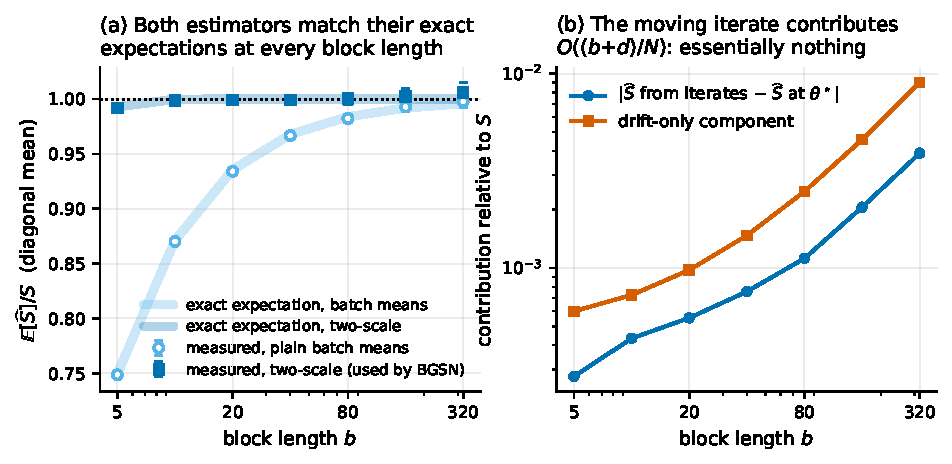
\includegraphics[width=\linewidth]{fig2_lrv.pdf}}{\fbox{\parbox{0.9\linewidth}{\centering\vspace{2em}\texttt{\detokenize{fig2_lrv}} pending\vspace{2em}}}}
\caption{\textbf{The long-run covariance estimator, and why the moving iterate does not
spoil it.} (a) Measured $\E[\widehat S]/S$ against block length: plain batch means follow
the closed-form bias $1-\Delta/(bS)$ (no fitted constants), while the two-scale form is
unbiased at every $b$, as \Cref{thm:lrv} predicts under geometric mixing.
(b) The algorithm's block gradients decomposed exactly into the score at $\ts$ and the
drift $\widehat H_t(\theta_{t-1}-\ts)$. The drift's contribution to $\widehat S$ is $0.1\%$
of $S$ at $b=20$ and $0.9\%$ at $b=320$, growing like $(b+d)/N$ as
\Cref{thm:lrv} predicts, and the estimator built from the algorithm's iterates is
indistinguishable from the one built at $\ts$. This is why our block length need only grow like $\log N$ rather than like a power of $N$ (\Cref{rem:whyfast}).}
\label{fig:lrv}
\end{figure}

%% Figure block, shared by ../paper/main.tex and ../submission/*.tex so the caption has
%% exactly one source.
\begin{figure}[t]
\centering
\IfFileExists{fig8_hard_design.pdf}{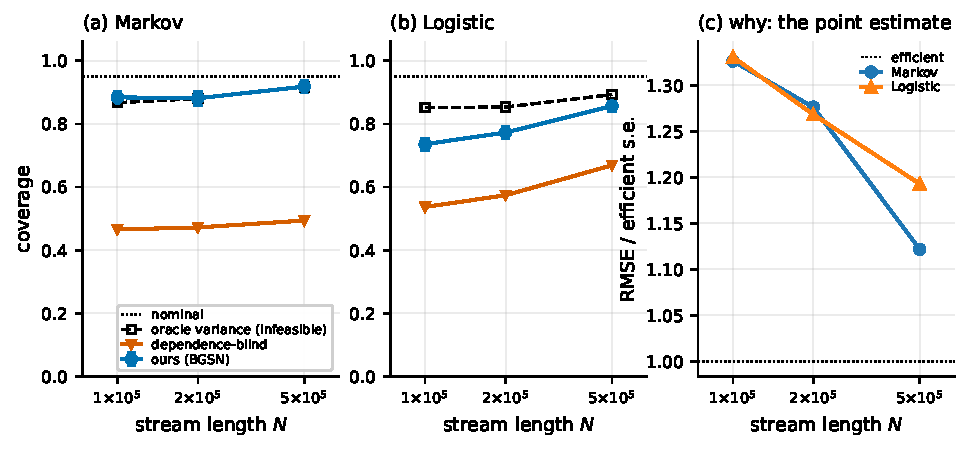
\includegraphics[width=\linewidth]{fig8_hard_design.pdf}}{\fbox{\parbox{0.9\linewidth}{\centering\vspace{2em}\texttt{\detokenize{fig8_hard_design}} pending\vspace{2em}}}}
\caption{\textbf{Separating ``the variance estimate is wrong'' from ``the central limit theorem
has not taken hold''} on the regime-switching design, whose covariate chain has an integrated
autocorrelation time of about $\HardTau$ observations. \textbf{(a)} Coverage of nominal $95\%$
intervals against $N$. The infeasible curve uses the exact $H^{-1}SH^{-1}$ at the same iterate,
so the vertical distance between it and ours is everything our covariance estimator is
responsible for; the largest such distance over the sweep is $\HardMaxGap$. Both rise towards
nominal; the dependence-blind curve does not. \textbf{(b)} The reason the left panel starts low:
the root-mean-square error of the point estimate, divided by the efficient standard error, is
still above one at small $N$, so $\sqrt N(\theta_T-\ts)$ is not yet close to its limit and no
choice of variance can give nominal coverage.}
\label{fig:hard}
\end{figure}

\IfFileExists{tab_hard.tex}{\begin{table}[tbp]
\centering
\small
\caption{\textbf{On the two designs whose point estimate has not converged, our interval tracks the infeasible oracle interval at every sample size} ($d=20$, $b=20$; $R$ decreases from 200 at the smallest $N$ to 150 at the largest, since what is being measured is the gap between the first two columns and a Monte Carlo standard error near $0.01$ is ample for it). \emph{ours} is \bgsn{}; \emph{oracle} uses the exact $H^{-1}SH^{-1}$ at the same iterate and is infeasible; \emph{blind} uses the i.i.d.\ plug-in. \emph{err} is the root-mean-square error divided by the efficient standard error, so $\mathrm{err}=1$ means the point estimate has reached the asymptotic regime, and \emph{clips} counts activations of the step-length safeguard out of $N/b$ blocks. At $N=200{,}000$ neither design is nominal because $\mathrm{err}>1$: the central limit theorem has not taken hold, which no variance estimator can repair. What our estimator is responsible for is the difference between the \emph{ours} and \emph{oracle} columns, and the largest such difference over both designs and all four sample sizes is $0.116$. The \emph{blind} column is the one that does not converge. Note that \emph{clips} does not grow with $N$, which is the empirical content of Proposition~\ref{prop:shift}.}
\label{tab:hard}
\begin{tabular}{lrccccr}
\toprule
design & $N$ & ours & oracle & blind & err & clips \\
\midrule
Markov & 100{,}000 & 0.884 & 0.867 & 0.466 & 1.33 & 8 \\
 & 200{,}000 & 0.881 & 0.880 & 0.472 & 1.28 & 8 \\
 & 500{,}000 & 0.918 & 0.917 & 0.494 & 1.12 & 7 \\
\midrule
Logistic & 100{,}000 & 0.736 & 0.852 & 0.537 & 1.33 & 2 \\
 & 200{,}000 & 0.773 & 0.853 & 0.574 & 1.27 & 2 \\
 & 500{,}000 & 0.857 & 0.893 & 0.669 & 1.19 & 2 \\
\bottomrule
\end{tabular}
\end{table}
}{}
\IfFileExists{tab_real.tex}{\begin{table}[t]
\centering
\small
\setlength{\tabcolsep}{4pt}
\caption{\textbf{Real hourly streams.} Protocol A: real covariates, synthetic autoregressive errors whose coefficient equals the AR(1) coefficient of the real residuals, so the target and the long-run covariance are exact conditionally on the covariate path. Protocol B: fully real response, target the full-stream $M$-estimator; because that target is estimated from a superset of each segment, the correct nominal level for this comparison is $2\Phi(z_{0.025}/\sqrt{1-1/R})-1$, reported in the header. Traffic: $n=8000$ per segment, $b=40$. Air quality: $n=10000$ per segment, $b=50$, pooled over 12 monitoring sites.}
\label{tab:real}
\begin{tabular}{lcccc}
\toprule
& \multicolumn{2}{c}{traffic (I-94)} & \multicolumn{2}{c}{air quality (PM2.5)} \\
\cmidrule(lr){2-3}\cmidrule(lr){4-5}
method & A: exact truth & B: full-stream target & A: exact truth & B: full-stream target \\
\midrule
\emph{nominal} & 0.950 & 0.976 & 0.950 & 0.994 \\
\midrule
\textbf{BGSN} (this paper) & 0.818 & 0.795 & 0.893 & 0.858 \\
\quad with plain batch means & 0.814 & 0.795 & 0.892 & 0.816 \\
\quad with the i.i.d.\ plug-in variance & 0.597 & 0.682 & 0.543 & 0.361 \\
streaming Newton, i.i.d.\ theory & 0.580 & 0.682 & 0.500 & 0.365 \\
ASGD + our long-run variance & 0.564 & 0.523 & 0.331 & 0.330 \\
ASGD, i.i.d.\ plug-in & 0.391 & 0.455 & 0.198 & 0.212 \\
ASGD + random scaling & 0.571 & 0.568 & 0.422 & 0.486 \\
oracle variance \emph{(infeasible)} & 0.773 & -- & 0.788 & -- \\
\midrule
\multicolumn{5}{l}{\emph{stream diagnostics}}\\
residual AR(1) coefficient & \multicolumn{2}{c}{0.756} & \multicolumn{2}{c}{0.909 (median over sites)} \\
$R^2$ & \multicolumn{2}{c}{0.782} & \multicolumn{2}{c}{0.327} \\
block-adequacy $r_j$ & 0.163 & 0.271 & 0.186 & 0.302 \\
\bottomrule
\end{tabular}
\end{table}
}{}
\IfFileExists{tab_wellcond.tex}{\begin{table}[tbp]
\centering
\small
\caption{\textbf{A well-conditioned dependent design isolates the inference question} ($\Sigma_x=I$, so $\mathrm{cond}(H)=1.00$; otherwise identical to the AR-hom column of \Cref{tab:main}: $d=20$, $N=200{,}000$, $b=20$, $\kappa=2.92$, $R=300$). Here every point estimator is efficient (\emph{err} $\approx1$), so coverage is decided by the covariance estimate alone. Averaged SGD with our long-run variance is calibrated; the same estimator with the i.i.d.\ plug-in is not, by the factor $\sqrt{\kappa}=1.71$ in width that Proposition~\ref{prop:coverage} predicts. On the ill-conditioned designs of \Cref{tab:main} the first-order baselines cannot be read this way, because there their point estimates have not converged.}
\label{tab:wellcond}
\resizebox{\ifdim\width>\linewidth\linewidth\else\width\fi}{!}{%
\begin{tabular}{lccc}
\toprule
method & cov & w & err \\
\midrule
\textbf{BGSN} (this paper) & \textbf{0.942} & 1.00 & 1.03 \\
\quad with plain batch means & 0.933 & 0.97 & 1.03 \\
\quad with the i.i.d.\ plug-in variance & 0.743 & 0.59 & 1.03 \\
streaming Newton, i.i.d.\ theory & 0.740 & 0.59 & 1.03 \\
ASGD + our long-run variance & 0.931 & 1.00 & 1.07 \\
ASGD, i.i.d.\ plug-in & 0.721 & 0.59 & 1.07 \\
ASGD + random scaling & 0.917 & 1.28 & 1.07 \\
AdaGrad + our long-run variance & \textbf{0.943} & 1.00 & 1.03 \\
oracle variance \emph{(infeasible)} & \textbf{0.941} & 1.00 & 1.03 \\
\bottomrule
\end{tabular}
}
\end{table}
}{}
\IfFileExists{tab_ablation.tex}{\begin{table}[tbp]
\centering
\small
\caption{\textbf{Ablations} on the homogeneous autoregressive design ($d=20$, $\kappa=2.92$, $R=250$). \emph{cov} columns are coverage of nominal 95\% intervals using the two-scale, plain batch-means, and i.i.d.\ plug-in variance respectively; \emph{eff} is the empirical variance of the point estimate divided by its asymptotic value ($1.00$ is efficient); \emph{adeq} is the free block-adequacy diagnostic $r_j$, an estimate of the relative block-length bias of plain batch means. The three coverage columns use the two-scale, plain batch-means and i.i.d.\ plug-in variance respectively. In panel~(i) the designs are abbreviated AR (autoregressive), AR-s (strongly autoregressive) and Mkv (regime-switching); the number of times the safeguard acted is in the text. Panel (c$'$) is on the regime-switching design and is the reason the default warm-up is $c_{\mathrm w}=200$ rather than $50$: there, $50d$ consecutive observations span only about thirty regime visits, the curvature estimate is still rank-starved, and the $1/t$ schedule diverges. The warm-up must span enough effectively distinct design points, which is not the same as enough observations. Panel (i) varies how the blocked step is safeguarded: \emph{none} is the raw $1/t$ step, \emph{cap} is the step-length safeguard of \eqref{eq:step} at $c_D=1$ (our default) with \emph{cap 0.25} and \emph{cap 4} changing $c_D$ by a factor of four either way, \emph{shift} is the rejected schedule shift of \Cref{app:t0}, and \emph{both} applies the two together; \emph{clips} counts how many of the $10{,}000$ blocks the safeguard acted on. \emph{eff} is in scientific notation where the unsafeguarded step diverges. Panel (j) is on a short stream ($N=4000$, $d=11$, the length of a real-data evaluation segment) and varies the cap on the warm-up as a fraction of the stream; $\varpi_{\mathrm w}=1$ means uncapped, which spends $2200$ of the $4000$ observations on curvature and leaves $45$ blocked steps.}
\label{tab:ablation}
\small
\setlength{\tabcolsep}{4pt}
\resizebox{\ifdim\width>\linewidth\linewidth\else\width\fi}{!}{%
\begin{tabular}{llrrrrr}
\toprule
panel & setting & eff & 2-scale & BM & plug-in & $r_j$ \\
\midrule
\multirow{5}{*}{(a) length $N$} & $N=25{,}000$ & 1.23 & 0.930 & 0.922 & 0.710 & 0.086 \\
 & $N=50{,}000$ & 1.08 & 0.937 & 0.931 & 0.731 & 0.072 \\
 & $N=100{,}000$ & 1.04 & 0.947 & 0.938 & 0.733 & 0.069 \\
 & $N=200{,}000$ & 1.04 & 0.947 & 0.937 & 0.736 & 0.069 \\
 & $N=400{,}000$ & 1.10 & 0.941 & 0.934 & 0.729 & 0.069 \\
\midrule
\multirow{8}{*}{(b) block $b$} & $b=5$ & 1.02 & 0.948 & 0.905 & 0.736 & 0.325 \\
 & $b=10$ & 1.03 & 0.949 & 0.926 & 0.737 & 0.149 \\
 & $b=20$ & 1.04 & 0.947 & 0.937 & 0.736 & 0.069 \\
 & $b=40$ & 1.04 & 0.946 & 0.943 & 0.737 & 0.041 \\
 & $b=80$ & 1.05 & 0.946 & 0.944 & 0.738 & 0.045 \\
 & $b=160$ & 1.06 & 0.946 & 0.944 & 0.734 & 0.060 \\
 & $b=320$ & 1.07 & 0.943 & 0.944 & 0.738 & 0.085 \\
 & $b=640$ & 1.10 & 0.938 & 0.942 & 0.733 & 0.118 \\
\midrule
\multirow{7}{*}{(c) warm-up} & $c_{\mathrm w}=0.5$ & 1.13 & 0.928 & 0.921 & 0.724 & 0.069 \\
 & $c_{\mathrm w}=5$ & 1.06 & 0.941 & 0.931 & 0.730 & 0.069 \\
 & $c_{\mathrm w}=25$ & 1.04 & 0.944 & 0.936 & 0.737 & 0.068 \\
 & $c_{\mathrm w}=50$ & 1.04 & 0.944 & 0.935 & 0.741 & 0.068 \\
 & $c_{\mathrm w}=100$ & 1.01 & 0.949 & 0.941 & 0.739 & 0.069 \\
 & $c_{\mathrm w}=200$ & 1.04 & 0.947 & 0.938 & 0.733 & 0.069 \\
 & $c_{\mathrm w}=500$ & 1.12 & 0.937 & 0.927 & 0.713 & 0.069 \\
\midrule
\multirow{4}{*}{(c$'$) warm-up, Mkv} & $c_{\mathrm w}=50$ & 2.19 & 0.848 & 0.812 & 0.452 & 0.239 \\
 & $c_{\mathrm w}=100$ & 1.76 & 0.879 & 0.851 & 0.467 & 0.238 \\
 & $c_{\mathrm w}=200$ & 1.41 & 0.907 & 0.877 & 0.495 & 0.237 \\
 & $c_{\mathrm w}=500$ & 1.21 & 0.923 & 0.900 & 0.536 & 0.235 \\
\midrule
\multirow{10}{*}{(d) ridge} & $c_\iota{=}0,\ \qr{=}0.2$ & 1.04 & 0.949 & 0.940 & 0.741 & 0.069 \\
 & $c_\iota{=}0.001,\ \qr{=}0.2$ & 1.04 & 0.949 & 0.940 & 0.740 & 0.069 \\
 & $c_\iota{=}0.01,\ \qr{=}0.2$ & 1.04 & 0.947 & 0.937 & 0.736 & 0.069 \\
 & $c_\iota{=}0.1,\ \qr{=}0.2$ & 1.04 & 0.931 & 0.920 & 0.703 & 0.069 \\
 & $c_\iota{=}1,\ \qr{=}0.2$ & 3.07 & 0.605 & 0.591 & 0.405 & 0.069 \\
 & $c_\iota{=}0.01,\ \qr{=}0.05$ & 1.03 & 0.943 & 0.931 & 0.729 & 0.069 \\
 & $c_\iota{=}0.01,\ \qr{=}0.1$ & 1.03 & 0.946 & 0.934 & 0.732 & 0.069 \\
 & $c_\iota{=}0.01,\ \qr{=}0.24$ & 1.04 & 0.948 & 0.938 & 0.737 & 0.069 \\
 & $c_\iota{=}0.01,\ \qr{=}0.4$ & 1.04 & 0.949 & 0.939 & 0.740 & 0.069 \\
 & $c_\iota{=}0.01,\ \qr{=}0.49$ & 1.04 & 0.949 & 0.940 & 0.740 & 0.069 \\
\midrule
\multirow{5}{*}{(e) $H_0$ scale} & $\lambda_0=1e-08$ & 1.04 & 0.947 & 0.937 & 0.736 & 0.069 \\
 & $\lambda_0=1e-06$ & 1.04 & 0.947 & 0.937 & 0.736 & 0.069 \\
 & $\lambda_0=0.0001$ & 1.04 & 0.947 & 0.937 & 0.736 & 0.069 \\
 & $\lambda_0=0.01$ & 1.04 & 0.947 & 0.937 & 0.736 & 0.069 \\
 & $\lambda_0=1$ & 1.03 & 0.947 & 0.935 & 0.734 & 0.069 \\
\midrule
\multirow{7}{*}{(f) curvature} & $m=1,\ p=1$ & 1.02 & 0.949 & 0.940 & 0.740 & 0.069 \\
 & $m=1,\ p=0.5$ & 1.02 & 0.949 & 0.940 & 0.739 & 0.069 \\
 & $m=1,\ p=0.2$ & 1.03 & 0.948 & 0.939 & 0.739 & 0.069 \\
 & $m=1,\ p=0.05$ & 1.03 & 0.948 & 0.937 & 0.737 & 0.069 \\
 & $m=1,\ p=1$ & 1.02 & 0.949 & 0.940 & 0.740 & 0.069 \\
 & $m=5,\ p=1$ & 1.03 & 0.949 & 0.938 & 0.737 & 0.069 \\
 & $m=20,\ p=1$ & 1.04 & 0.947 & 0.937 & 0.736 & 0.069 \\
\midrule
\midrule
\multirow{5}{*}{(g) strong dep.} & $b=20$ & 1.04 & 0.944 & 0.921 & 0.558 & 0.177 \\
 & $b=40$ & 1.05 & 0.946 & 0.934 & 0.556 & 0.082 \\
 & $b=80$ & 1.07 & 0.948 & 0.942 & 0.553 & 0.053 \\
 & $b=160$ & 1.09 & 0.947 & 0.946 & 0.555 & 0.063 \\
 & $b=320$ & 1.11 & 0.945 & 0.946 & 0.549 & 0.086 \\
\midrule
\multirow{3}{*}{(h) averaged} & $N=25{,}000$ & 1.28 & 0.923 & 0.916 & 0.701 & 0.079 \\
 & $N=100{,}000$ & 1.11 & 0.937 & 0.927 & 0.718 & 0.064 \\
 & $N=400{,}000$ & 1.13 & 0.939 & 0.930 & 0.725 & 0.067 \\
\midrule
\multirow{18}{*}{(i) safeguard} & AR, none & 1.05 & 0.947 & 0.937 & 0.733 & 0.069 \\
 & AR, shift & 1.07 & 0.942 & 0.935 & 0.729 & 0.069 \\
 & AR, cap & 1.04 & 0.947 & 0.937 & 0.736 & 0.069 \\
 & AR, cap 0.25 & 1.04 & 0.945 & 0.937 & 0.736 & 0.069 \\
 & AR, cap 4 & 1.04 & 0.948 & 0.937 & 0.736 & 0.069 \\
 & AR, both & 1.07 & 0.942 & 0.935 & 0.728 & 0.069 \\
 & AR-s, none & 1.22 & 0.922 & 0.897 & 0.537 & 0.177 \\
 & AR-s, shift & 1.12 & 0.936 & 0.911 & 0.527 & 0.177 \\
 & AR-s, cap & 1.04 & 0.944 & 0.921 & 0.558 & 0.177 \\
 & AR-s, cap 0.25 & 1.05 & 0.943 & 0.920 & 0.553 & 0.177 \\
 & AR-s, cap 4 & 1.05 & 0.943 & 0.918 & 0.559 & 0.177 \\
 & AR-s, both & 1.12 & 0.936 & 0.911 & 0.527 & 0.177 \\
 & Mkv, none & \ensuremath{1.1\times10^{14}} & 0.228 & 0.204 & 0.484 & 0.896 \\
 & Mkv, shift & 3.08 & 0.785 & 0.746 & 0.372 & 0.242 \\
 & Mkv, cap & 1.41 & 0.907 & 0.877 & 0.495 & 0.237 \\
 & Mkv, cap 0.25 & 1.59 & 0.883 & 0.848 & 0.480 & 0.237 \\
 & Mkv, cap 4 & \ensuremath{4.3\times10^{7}} & 0.518 & 0.484 & 0.526 & 0.520 \\
 & Mkv, both & 3.10 & 0.785 & 0.745 & 0.372 & 0.242 \\
\midrule
\multirow{5}{*}{(j) warm-up frac.} & $\varpi_{\mathrm w}=0.02$ & 1.40 & 0.937 & 0.946 & 0.723 & 0.190 \\
 & $\varpi_{\mathrm w}=0.05$ & 1.28 & 0.935 & 0.939 & 0.721 & 0.197 \\
 & $\varpi_{\mathrm w}=0.10$ & 1.28 & 0.929 & 0.930 & 0.715 & 0.203 \\
 & $\varpi_{\mathrm w}=0.25$ & 1.50 & 0.880 & 0.894 & 0.644 & 0.233 \\
 & $\varpi_{\mathrm w}=1.00$ & 2.51 & 0.787 & 0.789 & 0.515 & 0.281 \\
\bottomrule
\end{tabular}
}
\end{table}
}{}
\IfFileExists{tab_cost.tex}{\begin{table}[t]
\centering
\small
\caption{\textbf{Cost.} Wall-clock milliseconds for one pass over $N=200{,}000$ observations, single-threaded, median of 7 runs, and the empirical exponent $s$ in time $\propto d^{s}$ fitted on the four largest $d$. The i.i.d.\ plug-in score covariance that the independent-data theory prescribes costs $O(d^2)$ per \emph{observation}, so the dependence-blind interval is more expensive than our long-run interval, which costs $O(d^2)$ per \emph{block}.}
\ \emph{Asymptotic} exponents are the same exact counts evaluated at $N=10^{8}$, where the one-off $O(c_{\mathrm w}d^{3})$ warm-up is negligible and \eqref{eq:cost} reduces to $O(dN)$; at the $N$ used here the warm-up inflates the exponent, which is why the measured value exceeds one.}
\label{tab:cost}
\begin{tabular}{lrrrrrrrr}
\toprule
method & $d{=}5$ & $d{=}10$ & $d{=}20$ & $d{=}40$ & $d{=}80$ & $d{=}160$ & $s_{\mathrm{time}}$ & $s_{\mathrm{flop}}$ & $s_{\infty}$ \\
\midrule
\textbf{BGSN} (long-run interval) & 78.0 & 11.6 & 31.3 & 78.4 & 448.1 & 2697.5 & 2.18 & 1.56 & 1.00 \\
\quad with the i.i.d.\ plug-in variance & 43.4 & 79.6 & 241.6 & 632.2 & 2355.5 & 12448.9 & 1.90 & 1.91 & 1.86 \\
streaming Newton, Bernoulli $p=1/d$ & 46.3 & 21.3 & 15.1 & 169.5 & 457.7 & 2677.6 & 2.38 & 1.56 & -- \\
streaming Newton, every observation ($p=1$) & 77.0 & 292.8 & 840.9 & 2214.2 & 9754.7 & 46629.9 & 1.95 & 1.97 & 1.97 \\
ASGD (first order, random scaling) & 8.8 & 5.2 & 32.3 & 81.3 & 168.3 & 478.2 & 1.27 & -- & -- \\
offline HAC, $L=100$ \emph{(not streaming)} & 1568.3 & 2296.9 & 6894.0 & 21089.4 & -- & -- & -- & -- & -- \\
\bottomrule
\end{tabular}
\end{table}
}{}

%% Experimental results moved out of \Cref{sec:exp} to keep the main text short.  Nothing here is
%% duplicated in the main text.  Shared by ../paper/main.tex and ../submission/body.tex.

\subsection{The two designs whose point estimate has not converged}
\label{app:hard}

The Markov and Logistic columns need a caveat of their own, and it is the sharpest test of
whether our variance estimator is really doing the work we claim. Neither design's point estimate
has reached its asymptotic regime at $N=200{,}000$, for two different reasons. The Markov design's
regime chain has an integrated autocorrelation time of $\HardTau$ observations --- the sum
$1+2\sum_{k\ge1}$ of its autocorrelations, which is the factor by which dependence multiplies the
variance of a sample mean, so that $N$ dependent observations carry about as much information as
$N/\HardTau$ independent ones --- so its effective sample size is a small fraction of $N$ and the
point estimate is $\HardRmseSmall$ times the efficient standard deviation. On the Logistic design
the cause is the curvature rather than the dependence: the weight $\alpha=\sigma'(x^{\!\top}\theta)$
is largest at $\theta_0=0$, where the warm-up evaluates it, so $\Hb$ built there overestimates $H$
and the early steps are correspondingly too short; the point estimate is $\HardLogitRmseSmall$
times efficient and the fitted standard error is biased low with it. An interval built from the
\emph{correct} asymptotic variance must undercover in that situation, no matter who supplied
the variance, simply because $\sqrt N(\theta_T-\ts)$ is not yet close to its limit. So on these two designs the
question is not whether coverage is nominal but whether our interval matches the interval that
uses the exact $H^{-1}SH^{-1}$ at the same iterate. \Cref{tab:hard} and \Cref{fig:hard} answer it:
over a sweep in $N$ both rise towards nominal together while the dependence-blind interval does
not. On the Markov design the agreement is essentially exact: our coverage is within
$\HardMaxGapMarkov$ of the oracle's at every $N$, and at the top of the sweep, $N=\HardNBig$, both are
$\HardCovOursBig$ and $\HardCovOracleBig$ with the point estimate down to $\HardRmseBig$ times
efficient, against $\HardCovPluginBig$ for the dependence-blind interval. The direction of travel
is the whole point. Across the fivefold increase in $N$ our coverage and the oracle's move
together towards $0.95$ and stay within $\HardMaxGapMarkov$ of each other, while the
dependence-blind interval creeps up by a few hundredths towards its own asymptote, which
\Cref{prop:coverage} puts at $2\Phi(z_{0.025}/\sqrt{\KappaLoMarkov})-1$, far below nominal. We
stop the sweep at $N=\HardNBig$ rather than continuing to where coverage is nominal, because what
the experiment is for is the gap between the first two columns, and \Cref{tab:hard} shows that gap
is already at the level of the Monte Carlo standard error there. On the Logistic design
there is a real gap, and it is ours: our coverage is $\HardLogitCovOursSmall$ against the
oracle's $\HardLogitCovOracleSmall$ at $N=\HardNSmall$, a difference of $\HardLogitGapSmall$,
falling monotonically to $\HardLogitGapBig$ at $N=\HardNBig$, the top of the sweep. The cause is
visible in \Cref{tab:main}: our fitted width there is $\WidthRatioLogisticAbs$ times the oracle's,
i.e.\ the standard error is biased low, because $\Hb$ is an average over the whole stream and the
early blocks contribute $\alpha=\sigma'(0)=1/4$, its largest possible value, so $\Hb$
overestimates $H$ and $\Hb^{-1}S\Hb^{-1}$ underestimates the sandwich. That bias decays with the
Cesàro average of $\norm{\theta_t-\ts}$, which is why the gap closes; it is a finite-sample
property of averaging curvature along the path, it affects the base method identically, and no
choice of long-run covariance estimator would remove it. That is the signature we want: our error tracks
the oracle's at every sample size, and the dependence-blind error is the one that survives
$N\to\infty$. The step-length safeguard bound at most $\HardClipMax$ times per run anywhere in
that sweep, and the count does not rise with $N$, which is the empirical content of
\Cref{prop:shift}.

We report every design in \Cref{tab:main} at the same $N$ rather than tuning $N$ per design,
which is why the Markov column looks worst there; \Cref{tab:hard} is where that column is
resolved.

\paragraph{The step-length safeguard is what makes the hard design run at all.}
\Cref{tab:ablation}(i) varies the safeguard. With none, the autoregressive designs are barely
affected ($\ShiftEffArhomNone$ against $\ShiftEffArhomCap$ in relative variance) but the
regime-switching design diverges: relative variance $\ShiftEffMarkovNone$ against
$\ShiftEffMarkovCap$ with the safeguard, and coverage $\ShiftCovMarkovNone$ against
$\ShiftCovMarkovCap$. The safeguard is not doing this by damping the algorithm into submission:
it binds a median of $\ShiftClipMarkovCap$ times in $10{,}000$ blocks on that design and
$\ShiftClipArhomCap$ times on AR-hom, and \Cref{tab:hard} shows the count flat as $N$ grows by a
factor of five.

The constant $c_D$ behaves the way a safeguard constant should, which is to say it is irrelevant
until it is not. On AR-hom, changing it by a factor of four in either direction moves nothing
($\ShiftEffArhomCapLo$ at $c_D=1/4$ and $\ShiftEffArhomCapHi$ at $c_D=4$, against
$\ShiftEffArhomCap$ at our default $c_D=1$). On the design that actually needs the safeguard both
directions cost something, and asymmetrically: $c_D=1/4$ gives $\ShiftEffMarkovCapLo$ against
$\ShiftEffMarkovCap$ --- binding $\ShiftClipMarkovCapLo$ times instead of
$\ShiftClipMarkovCap$, it now restrains steps that were fine --- while $c_D=4$ is too loose to
prevent the blow-up at all and the relative variance is $\ShiftEffMarkovCapHi$. So $c_D$ is a
tuning constant with a real failure mode on one side, and we say so rather than advertising
insensitivity we only observe on the easy designs.

The schedule shift of \Cref{app:t0} is the alternative the contraction condition suggests more
directly, and it is measurably worse: $\ShiftEffMarkovShift$ against $\ShiftEffMarkovCap$ on the
regime-switching design, because it slows all $10^4$ steps to correct a handful. We report it
because we implemented it first, and because the comparison is the evidence for the design we
kept.

\subsection{The first-order baselines and the conditioning of the design}
\label{app:firstorder}

The first-order rows of \Cref{tab:main} need a caveat, and it cuts against us if we hide it.
These designs are ill-conditioned --- $\mathrm{cond}(H)=\CondArhom$ for AR-hom --- which is precisely
the regime streaming second-order methods exist for, and there averaged SGD's \emph{point}
estimate has not converged: its root-mean-square error is $\RmseAsgdArhom$ times the
efficient value against $\RmseBgsnArhom$ for \bgsn{}. Its intervals are therefore
uninformative about the inference question, whatever covariance they use. Two pieces of evidence show that this is about conditioning and not about our construction.
First, within \Cref{tab:main} itself: streaming AdaGrad, which rescales per coordinate, is
efficient on AR-het ($\RmseAdagradArhet$) and with our long-run variance it covers
$\CovAdagradArhet$ --- so the construction transfers to a first-order method as soon as that
method's point estimate converges. Second, \Cref{tab:wellcond} repeats the AR-hom design with
$\Sigma_x=I$, where every point estimator is efficient ($\WcRmseAsgd$ for averaged SGD,
$\WcRmseBgsn$ for \bgsn{}) and only the covariance can decide coverage: averaged SGD with our
long-run variance covers $\WcCovAsgdOurs$, the same estimator with the i.i.d.\ plug-in covers
$\WcCovAsgdPlugin$, and \bgsn{} covers $\WcCovBgsn$.

\subsection{Distributional accuracy beyond a single quantile}
\label{app:ks}

Coverage checks a single quantile, while the theorem claims a whole distribution, so we also
report the Kolmogorov--Smirnov distance between the studentised error (the error divided by
its own estimated standard error, which is what an interval implicitly compares to a normal
quantile)
$\sqrt N(\theta_{T,j}-\ts_j)/\{u_j^{\!\top}\Sft u_j\}^{1/2}$ and the standard normal, taken
per coordinate across replicates. On AR-hom the worst of the $d$ coordinates gives $\KsBgsnArhom$ against a $5\%$ critical value of
$\KsCritArhom$: marginally outside, so at this number of replicates the studentised distribution
is distinguishable from normal, and we report that rather than rounding it in our favour. The
dependence-blind studentisation gives $\KsPluginArhom$, an order of magnitude further out. The
comparison, not the test outcome, is the content: our studentisation is at the edge of detectable
non-normality while the dependence-blind one is not close. The standard errors themselves are accurate: $\SeRatioBgsnArhom$ times the
truth on average.

\subsection{Our estimator against an iterate-path estimator}
\label{app:obm}

Panel (a) puts our estimator and an iterate-path estimator on the same object, because an
interval uses the whole sandwich $\Sigma=H^{-1}SH^{-1}$ rather than $S$ alone. We compare our
composite $\Hb^{-1}\Sft\Hb^{-1}$, whose relative error falls with fitted exponent
$\RateExpSandwich$, with overlapping batch means on the \emph{iterate} path at the block length
its analysis prescribes --- the estimator of $\Sigma$ that uses no gradients and no curvature.

Two things must be said carefully here, because the comparison is easy to overstate. First, the
iterate-path estimator's relative error is flat over our range: the fitted exponent is
$\RateExpIterateObm$, and we do \emph{not} read that as its rate. Its published rate is
$N^{-1/8}$, which over a sixteenfold increase in $N$ predicts a reduction by a factor
$16^{-1/8}=0.71$ --- a change small enough that our range cannot separate it from zero, and our
fitted exponent should be treated as uninformative about it rather than as a measurement.
Second, what our range \emph{does} establish is the level, and the level is the practical
statement: over the whole range the iterate-path estimator's relative error in $\Sigma$ sits
near $\RateObmLevel$, which is not a usable standard error whatever its asymptotic rate, while
ours falls from $\RateOursLevelSmall$ to $\RateOursLevelBig$. We are comparing an estimator that
has entered its asymptotic regime with one that has not, and the honest claim is about the
sample sizes a practitioner would actually have, not about which exponent is larger.

\subsection{Curvature schedules}
\label{app:sched}

\RefGapFig{} compares deterministic gapping with Bernoulli thinning at a matched number of
rank-one updates, with the optimisation frozen at $\ts$ so that only estimation quality is
measured. The excess variance over the independent-data benchmark follows the two predicted
curves --- $O(\rho^{m})$ for gapping, $(\kappa_H-1)/m$ for thinning --- over more than an
order of magnitude in $m$. As stated in \Cref{sec:limits}, this is a curvature-side result:
\Cref{tab:ablation}(f) shows that the end-to-end effect on coverage is within Monte Carlo
error, which is what the theory predicts, since $\Hb$ enters the limit only through a rate.

Where gapping does pay is cost, and \Cref{tab:main} measures it. Compare \bgsn{} with the row
``base method with our long-run variance'': the two use the same variance estimator and the same
number of rank-one curvature updates per observation ($1/d$), and they cover the same
($\CovBgsnArhom$ against $\CovSniidtsArhom$ on AR-hom). They differ only in \emph{how} those
updates are placed --- on a deterministic gap of $m=d$ against Bernoulli retention with $p=1/d$.
At these settings the wall-clock difference is $\GapSpeedupArhom\times$, which is within our
timing noise, so we do not claim a speed-up: a gap avoids drawing and testing a random variable
per observation, but that saving is small next to the $O(d^2)$ update it guards. The case for
gapping is therefore the one \Cref{prop:gap} makes and \RefGapFig{} measures --- a strictly
better curvature estimate at a matched number of updates, $O(\rho^m)$ excess variance against
$(\kappa_H-1)/m$ --- together with the fact that it makes the per-block cost deterministic
rather than random. It is a better cost knob, not a faster one.
\subsection{Ablations}
\label{app:abl}

\RefAblFig{} and \Cref{tab:ablation} vary one design choice at a time.
(a) Coverage rises monotonically to nominal with $N$, and the gap to the dependence-blind
interval does \emph{not} close --- it converges to the predicted $0.749$.
(b) Coverage as a function of $b$ is flat for the two-scale estimator over
$b\in[10,320]$ and degrades at both ends for plain batch means (bias at small $b$, noise at
large $b$): the practical content of the $O(\rho^{b})$-versus-$O(1/b)$ distinction.
(c) The curvature warm-up matters, though less than it did before the step-length safeguard
absorbed part of its job: with essentially no warm-up, coverage on this design is
$\CovNoWarmup$ against $\CovBgsnArhom$ at the default, and above $c_{\mathrm w}\approx25$ the
result is insensitive. (c$'$) is where the warm-up is load-bearing: on the regime-switching
design the relative variance is $\WarmMarkovFifty$ at $c_{\mathrm w}=50$ against
$\WarmMarkovTwoHundred$ at $c_{\mathrm w}=200$, because there $50d$ consecutive observations span
only about thirty regime visits and leave the curvature estimate rank-starved. That is what sets
our default, and it is a statement about effectively distinct design points rather than about
observations.
(d) Results are insensitive to the ridge exponent $\qr$ over the whole admissible range, and to
the ridge constant $c_\iota$ from $0$ --- no ridge at all --- up to our default $0.01$; at
$c_\iota=0.1$ coverage slips by two points and at $c_\iota=1$ the ridge dominates the data terms
and the estimator is no longer efficient. So the ridge is safe to leave alone but not safe to
enlarge, and the honest reading is that the default sits at the top of the flat region rather than
in the middle of it. That $c_\iota=0$ works as well as the default is worth stating plainly: the
ridge is in the algorithm so that \Cref{lem:ridge} can hold for \emph{every} $t$ without an
assumption on the iterates, not because the runs need it.
(e) Results are insensitive to the initial curvature scale $\lambda_0$ over eight orders of
magnitude, which matters because that is a parameter a user would otherwise have to think about.
(f) Gap and thinning behave as \Cref{prop:gap} predicts and do not move coverage, which is
what the theory says: $\Hb$ enters the limit only through a rate.
(g) At strong dependence ($\phi=\psi=0.85$, $\kappa=\KappaStrong$) the two estimators separate in
exactly the way the $O(\rho^b)$-versus-$O(1/b)$ distinction predicts. Plain batch means need a
long block: coverage rises from $\StrongCovBmSmallB$ at $b=20$ to $\StrongCovBmBigB$ at $b=160$.
The two-scale correction does not: it is already at $\StrongCovFtSmallB$ at $b=20$ and stays there
($\StrongCovFtBigB$ at $b=160$). The free diagnostic $r_j$ falls from $\StrongAdeqSmallB$ to
$\StrongAdeqBigB$ over the same range, which is what makes it usable as a guide to whether plain
batch means would have been adequate. So the correction is what buys the short block, and the short
block is what keeps the estimator cheap.
(h) The weighted averaged variant is slightly better at small $N$ and slightly worse at
large $N$; both are reported.
The non-positive-definiteness fallback of \Cref{rem:psd} never triggered anywhere: the rate is
$0$ in every simulation and $\RealPsdFallback$ of coordinate-replicate pairs on the real streams,
where an earlier version of these experiments did not record it at all and where we would have
expected it if anywhere, since there the lag-one correction is largest. It never triggered
($0.0\%$ of all runs, all panels).
\subsection{Cost: the correct interval is also the cheaper one}
\label{app:costexp}

The authoritative statement is the operation count, because it is exact and independent of the
machine. The streaming pass grows as $d^{\StreamExpBgsn}$ for \bgsn{} and as
$d^{\StreamExpPlugin}$ once the i.i.d.\ plug-in variance is added, because the plug-in score
covariance costs $O(d^2)$ per \emph{observation} whereas our long-run covariance costs $O(d^2)$
per \emph{block}; evaluating the whole count at $N=10^{8}$ gives $d^{\AsymExpBgsn}$ against
$d^{\AsymExpPlugin}$. Those are the design claim, and they are arithmetic rather than a fit.

The exponents fitted at the $N$ of \Cref{tab:cost} are \emph{not} the streaming cost, and we
say so rather than quoting them as if they were: with $c_{\mathrm w}=200$ and $N=200{,}000$ the
one-off $O(c_{\mathrm w}d^3)$ warm-up dominates the $O(dN)$ pass for $d\ge40$
(the crossover is $N\gtrsim c_{\mathrm w}d^2$), so both measured exponents sit near $2$. What
is robust at this $N$ is the \emph{level}: the plug-in variant costs more than \bgsn{} in
wall-clock at every $d$ we tried, by a factor between $\CostRatioPluginLo$ and
$\CostRatioPluginHi$ (median $\CostRatioPlugin$), and in the main configuration \bgsn{}
runs in $\TimeRatioArhom$ times the time of the dependence-blind streaming Newton method --- that
is, our valid intervals cost less than the invalid ones, not more. The measured wall-clock
exponents, on a shared and heavily loaded machine, are $d^{\CostExpBgsn}$ and
$d^{\CostExpPlugin}$; they are noisier than the counts and we report them only as corroboration.
\RefCostFig{} plots the same timings against $d$, where the message is the vertical separation
rather than either slope.

\subsection{Choosing the block length on a real stream}
\label{app:realb}

\Cref{fig:real}(c) shows why the block length is the one parameter a practitioner must think
about on real data, and that the free diagnostic
$r_j=|u_j^{\!\top}(\Sft-\Sbm)u_j|/(u_j^{\!\top}\Sbm u_j)$ flags the problem. The denominator is
the batch-means quadratic form, not the two-scale one: $\Sbm$ is a sum of outer products and so
its quadratic forms are non-negative, whereas those of $\Sft$ can be negative
(\Cref{rem:psd}), and an earlier version of this diagnostic divided by the latter and produced
meaningless numbers on the real streams. On the traffic stream $r_j$ is
$\RealAdeqMetro$ at the $b=\RealBMetro$ we use, and the sweep in \Cref{fig:real}(c) shows what it is
good for: $r_j$ is U-shaped in $b$, rising both for short blocks, where plain batch means carry the
$O(1/b)$ bias, and for long ones, where too few blocks remain for a stable estimate. Our coverage
over that fortyfold range in $b$ is flat and stays within a few hundredths of the infeasible
oracle-variance curve, which is the evidence that the shortfall from nominal on these segments is
the point estimate rather than the covariance. So $r_j$ is a guide to choosing $b$, not a
calibration guarantee, and we do not claim it predicts coverage.


\section{Safeguarding the blocked step}
\label{app:shift}

\begin{proof}[Proof of \Cref{prop:shift}]
On $\mathcal A$ there are finitely many $t$ at which $\Pi_t$ is active, so
$T_0=\max\{t:\Pi_t\text{ active}\}$ is finite and for $t>T_0$ the recursion is
$\theta_t=\theta_{t-1}-\gamma_t\Hb_{t-1}^{-1}\gb_t(\theta_{t-1})$ verbatim. Two sequences that
agree from a finite index on have the same limit points, the same almost sure rate and the same
limit law, since all three are tail properties; the initial condition at $T_0$ is a finite random
vector, and \Cref{thm:as,thm:rate,thm:clt} hold for the recursion started from any initial
condition (\Cref{as:ident} is global). For the last claim, if $\theta_t\to\ts$ and
$\norm{\gamma_t\Hb_{t-1}^{-1}\gb_t(\theta_{t-1})}\to0$ almost surely then for almost every
$\omega$ there is $T_1(\omega)$ beyond which
$\norm{\gamma_t\Hb_{t-1}^{-1}\gb_t}<c_D(1+\norm{\ts})/2\le c_D(1+\norm{\theta_{t-1}})$, so
$\Pi_t$ is inactive for $t>T_1$ and $\omega\in\mathcal A$.
\end{proof}

\noindent
We repeat here what \Cref{sec:setting} says, because it is the kind of gap a reader is entitled
to be told about twice. \Cref{prop:shift} is conditional on $\mathcal A$ and does not establish
$\Prob(\mathcal A)=1$ unconditionally: the implication runs from convergence to eventual
inactivity, not the other way. The reason we do not close the loop is that the safeguard factor
$\min\{1,c_D(1+\norm{\theta_{t-1}})/\norm{v}\}$ depends on $\gb_t$, hence is $\mathcal F_t$- and
not $\mathcal F_{t-1}$-measurable, and multiplying the noise term $\gamma_t\Hb^{-1}\eps_t$ by an
$\mathcal F_t$-measurable factor destroys the martingale-difference property that
\Cref{thm:as,thm:clt} rest on. Two routes would close it and both are outside our scope: the
expanding-truncation construction of \citet{kushner2003stochastic} and
\citet{andrieu2005stability}, which replaces the cap by a projection onto a ball of radius
increasing with the number of activations and proves the activation count finite; or an
$\mathcal F_{t-1}$-measurable variant that caps using the \emph{previous} block's amplification,
$\gamma_t\wedge\tau/\opnorm{\Hb_{t-2}^{-1}\Hh_{t-1}}$, which is predictable and so leaves the
martingale structure intact, at the cost of an extra $O(d^2)$ per block. What we do instead is
report the activation counts, which are between $2$ and $7$ per run and do not grow with $N$.

\subsection{The step-size shift: the alternative we implemented and rejected}
\label{app:t0}

The variant replaces the step sequence $\gamma_t=c\,t^{-a}$ of \eqref{eq:step} by
$\gamma_t=c\,(t+t_0)^{-a}$ with
\begin{equation}
t_0=\max\Big\{0,\ \tfrac{c}{2}\max_{t\le \Tw}\opnorm{\Hb_{\Tw}^{-1}\Hh_t}-1\Big\},
\label{eq:t0}
\end{equation}
$\Tw=\lceil c_{\mathrm w}d/b\rceil$ being the last warm-up block, and switches the step-length
safeguard $\Pi_t$ off. By construction \eqref{eq:contract} then holds at $t=1$ for every block
whose amplification does not exceed the warm-up maximum. The spectral norms are obtained by four
power iterations per warm-up block with $\Hh_t$ applied in factored form, so no $d\times d$
product is formed and the whole computation costs
$O(c_{\mathrm w}(d^2+db)\,d/b)$ flops once, $O(1)$ in $N$; with $b=m=d$ that is
$O(c_{\mathrm w}d^2)$, some $4$--$5\%$ of the total at the settings of \Cref{tab:cost}. Setting
\texttt{t0\_mult}$\,=0.5$ and \texttt{step\_cap}$\,=0$ in the code selects this variant.

\begin{proof}[Correctness of the rejected shift variant]
Write $\Tw$ for the last warm-up block. For every $t\le\Tw$,
$\opnorm{\Hb_{\Tw}^{-1}\Hh_t}\le\opnorm{\Hb_{\Tw}^{-1}}\opnorm{\Hh_t}$. The first factor is
finite almost surely by \Cref{lem:ridge}, which bounds it by $c_1^{-1}n_{\Tw}^{\qr}$ using only
the ridge in \eqref{eq:curv} and no property of the iterates. The second is finite almost
surely because $\opnorm{\Hh_t}\le b^{-1}\sum_{i\in B_t}\alpha_i\norm{\Psi_i}^2$ and
\Cref{as:curv} gives $\E\opnorm{\alpha\Psi\Psi^{\!\top}}^{\eta'}\le C_{\eta'}$ with
$\eta'>2$, so each summand is finite a.s.\ and the maximum is over the finitely many blocks
$t\le\Tw$. Hence $t_0<\infty$ a.s. Measurability with respect to
$\mathcal{F}_{\Tw}=\sigma(\xi_1,\dots,\xi_{b\Tw})$ is immediate: \eqref{eq:t0} is a function of
$\Hb_{\Tw}$ and of $\{\Hh_t\}_{t\le\Tw}$, all of which are built from the warm-up window and
from $\theta_0$, and the warm-up takes no parameter step.

For the second claim, fix $\omega$ in the almost sure event $\{t_0<\infty\}$ and let
$K=\lceil t_0\rceil$. Then $c(t+t_0)^{-a}\ge c(t+K)^{-a}$, and
$\sum_{t\ge1}(t+K)^{-a}=\sum_{t>K}t^{-a}=\infty$ for $a\le1$, so $\sum_t\gamma_t=\infty$.
Likewise $c(t+t_0)^{-a}\le ct^{-a}$, so $\sum_t\gamma_t^{1+\delta}\le
c^{1+\delta}\sum_t t^{-a(1+\delta)}<\infty$ whenever $a(1+\delta)>1$, which is the same
condition as for the unshifted sequence. Finally $(t+t_0)^{-a}/t^{-a}=(1+t_0/t)^{-a}\to1$.
Conditioning on $\mathcal{F}_{\Tw}$ is harmless because $\mathcal{F}_{\Tw}$ is generated by
finitely many observations, so it changes no tail statement and, by \Cref{as:mix}, leaves the
stream after the warm-up geometrically mixing with the same constants up to a factor.

\Cref{thm:as} and the preliminary rate use the step sequence only through
$\sum_t\gamma_t=\infty$ and $\sum_t\gamma_t^2\opnorm{P_{t-1}}^2<\infty$, both just verified, so
they transfer immediately. \Cref{thm:rate,thm:clt} and \Cref{prop:blockfree} deserve one extra
line, because their proof uses the identity $\gamma_t=1/t$ explicitly in the Abel summation
\eqref{eq:abel}, and we would rather write the shifted identity out than assert that nothing
changes. With $\gamma_t=(t+t_0)^{-1}$, multiplying
$\delta_t=\delta_{t-1}-\gamma_tP_{t-1}\{H\delta_{t-1}+\eps_t+r_t\}$ by $t+t_0$ gives
\begin{equation}
(t+t_0)\,\delta_t=(t-1+t_0)\delta_{t-1}+(I-P_{t-1}H)\delta_{t-1}-P_{t-1}\eps_t-P_{t-1}r_t ,
\label{eq:abelshift}
\end{equation}
which is \eqref{eq:abel} with $t$ replaced by $t+t_0$ throughout. Summing from $t=1$ to $T$ now
telescopes to $(T+t_0)\delta_T=t_0\delta_0+\sum_{t\le T}\{\cdot\}$ instead of
$T\delta_T=\sum_{t\le T}\{\cdot\}$, so dividing by $T+t_0$,
\[
\delta_T=\frac{t_0\,\delta_0}{T+t_0}
\;-\;\frac{1}{T+t_0}H^{-1}\sum_{t\le T}\eps_t
\;+\;\frac{T}{T+t_0}\big\{(\mathrm A)+(\mathrm B)-(\mathrm C)\big\},
\]
with $(\mathrm A)$, $(\mathrm B)$, $(\mathrm C)$ exactly as in the unshifted proof. Two
differences from \eqref{eq:abel}, and both are negligible. The new first term is
$O(t_0/T)=O(1/T)=o(T^{-1/2})$ because $t_0$ is a finite constant, so it does not enter the
limit. And $T/(T+t_0)=1+O(1/T)$ and $(T+t_0)^{-1}=T^{-1}(1+O(1/T))$, so every term of the
unshifted decomposition is multiplied by $1+O(1/T)$; since each of them is $O_p(T^{-1/2})$ or
smaller, the perturbation is $O_p(T^{-3/2})$. The remaining estimates --- the bounds on
$(\mathrm A)$, $(\mathrm B)$ and $(\mathrm C)$, the martingale central limit theorem applied to
$T^{-1/2}\sum_{t\le T}\eps_t$, and the Gordin decomposition --- do not involve $\gamma_t$ at
all. Hence the rate, the block-freeness statement and the limit law are unchanged. So the shift
variant has the cleaner theory of the two; it is the empirical comparison, not the theory, that
made us prefer the safeguard.
\end{proof}

\noindent
Two remarks on what this variant does and does not do. First, \eqref{eq:t0} does not make
\eqref{eq:contract} hold for \emph{every} $t$: the maximum in \eqref{eq:t0}
is over warm-up blocks, so a later block with an unusually badly conditioned $\Hh_t$ can still
violate \eqref{eq:contract} at that single $t$. What the shift buys is that the violation
happens with $\gamma_t\le(1+t_0)^{-1}$ rather than $\gamma_1=1$, so a single bad block moves
$\theta$ by a bounded multiple of its distance to $\ts$ instead of by a large one, and the
recursion recovers. Second, the proposition is about asymptotics; the finite-sample effect of
the shift is a trade, because a larger $t_0$ also slows the decay of the initial condition,
which decays like $t_0/(T+t_0)$ rather than $1/T$. This is why we set $t_0$ from
\eqref{eq:contract} --- the smallest value that restores contraction --- rather than by taking a
comfortable margin, and why \Cref{tab:ablation} reports the sensitivity.

%% Material moved out of \Cref{sec:setting} to keep the main text short.  Included from the
%% appendix (\Cref{app:shift}); shared by ../paper/main.tex and ../submission/body.tex.

\subsection{Where the contraction condition comes from, and why it fails}
\label{app:contract}

Linearising \eqref{eq:step} at $\ts$ and ignoring $\Pi_t$ gives the error recursion
\begin{equation}
\theta_t-\ts=\big(I-\gamma_t\Hb_{t-1}^{-1}\Hh_t\big)(\theta_{t-1}-\ts)
             -\gamma_t\Hb_{t-1}^{-1}\eps_t+o(\norm{\theta_{t-1}-\ts}).
\label{eq:err}
\end{equation}
Since $\Hb^{-1}\Hh_t$ is a product of two positive semidefinite matrices its eigenvalues are real and
non-negative, so the spectral radius of the linear map in \eqref{eq:err} is below one exactly when the
first inequality of \eqref{eq:contract} holds; the second is sufficient because
$\lambda_{\max}\le\opnorm{\cdot}$. We work with the operator norm because it is what we can compute and
because it is the conservative choice, and we say ``spectral radius'' rather than ``contraction''
deliberately: for a non-symmetric map a spectral radius below one bounds the \emph{asymptotic} growth of
powers, not the norm of a single step. What \eqref{eq:contract} rules out is the regime we actually
observe, in which $\gamma_t\lambda_{\max}\gg2$ and a single step multiplies the error by a large factor.

The per-block maxima of $\opnorm{H^{-1}\Hh_t}$ at $b=20$ are $55$ on the autoregressive design and $89$
on the regime-switching design, so the autoregressive designs are lucky rather than safe. Taking a
full-length step under those numbers makes the first iterates overshoot by orders of magnitude, and
because $\gamma_t=1/t$ undoes an excursion only at rate $1/t$, at realistic $N$ an overshoot in the
first few blocks can survive to the end of the stream. That is the mechanism behind the divergence
reported in \Cref{tab:ablation}(i): without the safeguard, two of six replicates on the
regime-switching design diverge outright, and none with it. This is not a defect of the base method ---
it is created by \emph{blocking} the gradient, which is the one thing we add.

\subsection{What \texorpdfstring{\Cref{prop:shift}}{the safeguard proposition} does not prove}
\label{app:notproved}

The obstruction is real and worth naming: the factor
$\min\{1,c_D(1+\norm{\theta_{t-1}})/\norm{v}\}$ depends on the current block's gradient, so it is
$\mathcal F_t$- rather than $\mathcal F_{t-1}$-measurable and correlates with the noise, which
breaks the martingale structure the proofs use. A complete treatment is available in the
stochastic-approximation literature on expanding truncations
\citep{andrieu2005stability,kushner2003stochastic}, at the price of machinery we do not need here.
\Cref{app:shift} gives the two concrete routes that would close the gap. A unit test asserts the
measured activation counts.

\subsection{The alternative we rejected, and why}
\label{app:rejected}

The contraction condition \eqref{eq:contract} suggests a different
remedy: shift the schedule to $\gamma_t=(t+t_0)^{-1}$ with
$t_0=\tfrac12\max_{t\le\Tw}\opnorm{\Hb_{\Tw}^{-1}\Hh_t}$ measured on the warm-up blocks, which
makes \eqref{eq:contract} hold at $t=1$ by construction and has a cleaner proof (it is a finite
deterministic reindexing; see \Cref{app:shift}). We implemented it and it is worse, for a reason
worth stating: it slows \emph{every} step, whereas the overshoot needs correcting on only a
handful. On the regime-switching design at $N=200{,}000$ the shift leaves the relative variance at
$\ShiftEffMarkovShift$ against $\ShiftEffMarkovCap$ for the safeguard, and on a stream short enough
that $t_0$ is comparable to the number of steps --- which is the case for our real-data segments --- it freezes the estimator
altogether. Both variants are in the code and both are reported
(\Cref{tab:ablation}(i)); the safeguard is the default.



\subsection{Sizing the curvature warm-up}
\label{app:warmup}

It matters: on a $4000$-observation stream with $d=11$, spending $c_{\mathrm w}d=2200$
observations on curvature leaves $\WarmFracStepsUncapped$ blocked steps and a relative variance of
$\WarmFracEffUncapped$, whereas capping at $10\%$ leaves $\WarmFracStepsCapped$ steps and a
relative variance of $\WarmFracEffCapped$ (\Cref{tab:ablation}(j)). Our real-data segments are of exactly that length.

\subsection{Cost accounting for the one-off terms}
\label{app:costdetail}

The warm-up performs $c_{\mathrm w}d$ rank-one updates at $O(d^2)$ each, which is the unavoidable cost
of producing a $d\times d$ curvature estimate at all and is of the same order as a single matrix
factorisation. The step-size shift of \Cref{app:t0} adds a further one-off
$O(c_{\mathrm w}(d^2+db)d/b)$, which is $4$--$5\%$ of the total operation count at the settings of
\Cref{tab:cost} and vanishes relative to the streaming pass as $N$ grows. \Cref{tab:cost} reports the
crossover $N\gtrsim c_{\mathrm w}d^2$ explicitly rather than hiding it in the constant.

\subsection{Dependence in the covariates is not enough}
\label{app:mds}

\begin{remark}[Dependence in the covariates is not enough]
\label{rem:mds}
If the conditional law of $y$ given $x$ is correctly specified and its innovations are
independent over time, then $(g_i)$ is a martingale difference sequence and $S=\Gamma_0$
\emph{exactly}, however persistent $x$ is. A genuine long-run-variance problem needs the
\emph{score} to be serially correlated: serially correlated errors, a latent dynamic
factor, or omitted dynamics. All our designs therefore couple dependent covariates with a
dependent error or latent process, and we report the resulting $\kappa_j$ explicitly.
Covariate dependence still matters for the effective sample size of the curvature
estimate, which is what \Cref{prop:gap} is about.
\end{remark}

\subsection{Misspecification and where dependence has to live}
\label{app:misspec}

In more detail, nothing in the analysis requires the model to be correctly specified: all that is used is that $\ts$ solves
$\nabla F(\ts)=0$ for the \emph{working} loss, so under misspecification $\ts$ is the pseudo-true
parameter and $H^{-1}SH^{-1}$ the corresponding long-run sandwich
\citep{white1982mle,domowitz1982misspecified}. That matters here, because omitted dynamics are one
of the commonest ways for a score to become serially correlated --- and correlated \emph{scores},
not merely correlated covariates, are what the problem requires. If the conditional law of $y$ given
$x$ is correctly specified with innovations independent over time, then $(g_i)$ is a martingale
difference sequence and $S=\Gamma_0$ \emph{exactly}, however persistent $x$ is (\Cref{rem:mds}). All
our designs therefore couple dependent covariates with a dependent error or latent process, and we
report the resulting $\kappa_j$ explicitly.


This matters in practice, because omitted dynamics are one of the commonest ways for a score to become
serially correlated \citep{white1982mle,domowitz1982misspecified}.

\subsection{Why the ridge scale is frozen}
\label{app:freeze}

With $\varsigma_\star$ fixed, positive and finite almost surely under \Cref{as:curv}, \Cref{lem:ridge}
holds unconditionally --- for every $t$, with no assumption on the iterates. The scale exists only to make
$c_\iota$ dimensionless; setting $\varsigma_\star=1$ recovers an unscaled ridge, and
\Cref{tab:ablation}(d) shows the results are the same.


\section{Extended related work}
\label{app:related}

\input{sec_related_detail}

\section{Extended discussion of the limitations}
\label{app:limits}

%% The full discussion of each limitation, moved out of \Cref{sec:limits} to keep the main text
%% short.  Shared by ../paper/main.tex and ../submission/body.tex.
We list the boundaries of the result plainly, because several of them are load-bearing.

\paragraph{Memory is $O(d^2)$, not $O(d)$.}
The $O(dN)$ claim is about \emph{time}. The method stores a $d\times d$ inverse curvature
estimate and two $d\times d$ covariance accumulators, so memory is $O(d^2)$; this is
inherited from the independent-data method we extend and is not something we improve. For
$d$ in the thousands this is the binding constraint, and a sketched or diagonal-plus-low-rank
curvature representation---as in \citet{kuang2026online,wang2026inference,godichonbaggioni2026complexity}---%
would be the natural remedy. Whether the block-gradient long-run covariance estimator
survives such a compression is open.

\paragraph{Geometric mixing is a real restriction, and the block length has to respect it.}
\Cref{thm:lrv} buys $b\asymp\log N$ from the geometric decay in
\Cref{lem:davydov}. Under algebraic mixing the flat-top bias is polynomial rather than
exponential and the admissible $b$ grows accordingly; long-memory streams are outside the
theory altogether. This is not merely formal: our air-quality stream has a residual lag-one
autocorrelation of $\RealAcfAirq$ and a median variance-inflation factor of $\RealKappaAirq$, and there the
block length needed for calibrated intervals is an order of magnitude larger than for the
traffic stream (\Cref{tab:real}). The free diagnostic
$r_j=|u_j^{\!\top}(\Sft-\Sbm)u_j|/(u_j^{\!\top}\Sft u_j)$ detects the problem---it estimates
the relative block-length bias of plain batch means---but it does not remove it. It could be
turned into an automatic rule by maintaining covariance accumulators at several block scales
$b,2b,4b,\dots$ at once (one extra $O(d^2)$ update per block per scale, all from the same
block gradients) and reporting from the smallest scale at which $r_j$ falls below a
tolerance; we did not implement this, and we do not claim an automatic rule for $b$.

\paragraph{$\Sft$ need not be positive semidefinite.}
This is intrinsic to flat-top and lugsail estimators \citep[Remark~5]{singh2025utility}.
Marginal intervals need only positive scalars $u_j^{\!\top}\Sft u_j$. The documented fallback to
$\Sbm$ never triggered in any simulation, but it does trigger on the real streams --- at a rate
of $\RealPsdFallback$ of coordinate-replicate pairs --- which is what one should expect, since
there the two designs are ill-conditioned and the lag-one correction is comparable to the
batch-means term. We report the rate rather than claiming it away, and a user who needs the full
matrix (for a joint test, say) must project it.

\paragraph{The curvature form is required.}
Everything rests on
$\nabla^2F(\theta)=\E[\alpha\,\Psi\Psi^{\!\top}]$, which holds for generalised linear
models, ridge and softmax regression, the geometric median and Gauss--Newton problems, but
not for a general objective. Without it there is no rank-one recursion and no
inversion-free update.

\paragraph{Warm-up is a real requirement, not an implementation detail.}
The $1/t$ schedule with a poor preconditioner leaves a slowly decaying component in the error.
On the autoregressive design the effect is now mild --- with a negligible warm-up, coverage of
nominal $95\%$ intervals is $\CovNoWarmup$ rather than $\CovBgsnArhom$ --- because the
step-length safeguard absorbs most of what a bad preconditioner does. On the regime-switching
design it is not mild: the relative variance is $\WarmMarkovFifty$ at $c_{\mathrm w}=50$ against
$\WarmMarkovTwoHundred$ at $c_{\mathrm w}=200$ (\Cref{tab:ablation}(c$'$)). We give a scaling rule
($c_{\mathrm w}d$ curvature updates, with $c_{\mathrm w}=200$ throughout) and show
insensitivity above it, but this is a tuning constant, and the asymptotic theory is silent
about it. What sets its size is not the number of observations but the number of effectively
distinct design points they span: on a persistent regime-switching stream, $50d$ consecutive
observations cover only about thirty regime visits, and the curvature estimate is still
rank-starved (\Cref{tab:ablation}(c$'$)). The warm-up also has a cost consequence we state
rather than bury: it performs $c_{\mathrm w}d$ rank-one updates at $O(d^2)$ each, so the total
time is $O(dN+c_{\mathrm w}d^3)$ and the advertised $O(dN)$ only bites once
$N\gtrsim c_{\mathrm w}d^2$. With $c_{\mathrm w}=200$ and $d=40$ that means
$N\gtrsim3\times10^5$, so at the $N=2\times10^5$ of \Cref{tab:cost} the warm-up dominates the
streaming pass for every $d\ge40$ we report, which is why that table separates the streaming
count from the total.

\paragraph{Blocking creates a stability condition, and our fix is not fully proved.}
The contraction condition $\gamma_t\opnorm{\Hb^{-1}\Hh_t}<2$ is a consequence of blocking the
gradient, so it is a cost of our construction and not of the method we build on. The step-length
safeguard in \eqref{eq:step} removes the failure it causes, and \Cref{prop:shift} shows that on
the event where the safeguard is eventually inactive it changes no asymptotic statement. What we
do \emph{not} prove is that this event has probability one: the implication we establish runs
from convergence to eventual inactivity, not back, because the safeguard factor depends on the
current block's gradient and so is not predictable, which breaks the martingale structure the
proofs use. \Cref{app:shift} says exactly what would close the gap --- an expanding-truncation
construction \citep{kushner2003stochastic,andrieu2005stability}, or a predictable variant that
caps using the previous block's amplification at an extra $O(d^2)$ per block --- and we did
neither. Instead we report the activation counts, which are between $2$ and $7$ per run and flat
in $N$ across every design and sample size in \Cref{tab:ablation,tab:hard}. Two further caveats.
The condition itself comes from the linearised recursion \eqref{eq:err}, so it is a heuristic for
non-quadratic objectives, exact only in the linear-model case. And $c_D$ is a tuning constant with a genuine failure mode:
\Cref{tab:ablation}(i) shows it is irrelevant over a factor of sixteen on the designs that do not
need the safeguard, but on the one that does, $c_D=4$ is too loose to prevent the blow-up. The
asymptotic theory says nothing about it, and we have no rule for choosing it beyond the value that
worked across our designs.

\paragraph{The central limit theorem is proved for fixed $b$, and we recommend growing $b$.}
\Cref{thm:clt} is unconditional at each fixed block length, but \Cref{thm:lrv} takes
$b\asymp\log N$, so the interval we recommend sits in the triangular-array regime where our proof
needs an extra hypothesis: that the finite random constants in \Cref{lem:series} are bounded in
probability uniformly in $N$ along the sequence $b_N$. We state that hypothesis in
\Cref{thm:clt} rather than hiding it, and we do not verify it. Closing the gap means redoing
\Cref{lem:series} with constants explicit in $b$; the naive route --- bounding
$\E\opnorm{H^{-1}-P_{t-1}}\norm{\eps_t}$ directly --- is the one the appendix shows loses a factor
$T^{1/2}$, which is why Gordin's decomposition is there in the first place. Two things make us
believe the composition is sound in practice rather than merely convenient: growing $b$ makes the
block scores less dependent, not more, so the mechanism the constants come from is working in our
favour; and coverage is flat in $b$ over $b\in[10,320]$ at $N=200{,}000$
(\Cref{tab:ablation}(b)), which is the statement the two theorems need to compose.

\paragraph{Rates and what we do not prove.}
We give an almost sure rate and a central limit theorem, not a Berry--Esseen bound; the
first-order Markovian literature has the latter for linear stochastic approximation
\citep{samsonov2025statistical}, and we do not match it. We attain the semiparametric
efficiency bound of \citet{li2023markovian} rather than establishing it. Our
$\widetilde O(N^{-1/2})$ rate for $\Sft$ is not comparable to the minimax rate
$\Theta(N^{-(1-a)/2})$ for Hessian-free covariance estimation from an iterate path
\citep{ni2026online}, because we use more information (block gradients and a maintained
curvature estimate) and because our step exponent is $a=1$, outside the range that bound is
stated for. Within the Hessian-free class the bound is close to attained
\citep{wei2026refining}, so the gap we report is about the information used, not about slack in
their analysis. We make no claim of optimality within our own information set: we do not know
the minimax rate for estimators that may use block gradients and a running curvature estimate.

\paragraph{Scope of the empirical evidence.}
All designs are convex $M$-estimation with $d\le160$ and $N\le4\times10^5$; there is no
deep-learning experiment and the theory would not support one. The dependence in the
simulated designs is stationary and geometrically decaying by construction. On the real
streams we do not know the truth, which is why we run two protocols; the semi-synthetic
protocol has an exact target but a synthetic (autoregressive) error process, and the fully
real protocol has a real error process but a target that is itself estimated---we correct
the nominal level for that exactly, but the correction assumes the segments are
approximately exchangeable, which non-stationarity would violate. Neither protocol alone
would be convincing; together they bracket the honest answer.

\paragraph{One thing we deliberately do not claim.}
Gapping improves the curvature estimate at matched cost (\Cref{prop:gap}, \RefGapFig{}),
but the curvature estimate enters the limit distribution only through a rate, so the
end-to-end effect on the point estimate and on coverage is second order and we could not
measure it reliably. The case for gapping is that it is free, deterministic, and provably
better than the randomised alternative---not that it changes the headline numbers.



\end{document}
